% -------------------------------------------------------------------
% This is the main file for the template of doctoral thesis at
% University of Split, Faculty of Electrical Engineering, Mechanical Engineering 
% and Naval Architecture in Split, Croatia.
% Initial version was created in March 2013, last update was in September 2016.

% Author: Toni Perkovi�, toperkov@fesb.hr, toperkov@unist.hr
% Author: Marin Bugari�, mbugaric@fesb.hr
% Author: Ivo Stan�i�, istancic@fesb.hr
% FESB 2016;
% -------------------------------------------------------------------

%%%%%%%%%%%%%%%%%%%%%%%%% POSTAVKE / SETTINGS %%%%%%%%%%%%%%%%%%%%%%%%%%%%%
\documentclass[12pt, twoside, onecolumn]{book}
%\usepackage{etex}
\usepackage[a4paper, top=2.5cm, bottom=2.5cm, left=3.0cm, right=2.5cm]{geometry}
\usepackage[absolute]{textpos}
\setlength{\TPHorizModule}{10mm}
\setlength{\TPVertModule}{\TPHorizModule}
\textblockorigin{0mm}{0mm}
%\usepackage{latexsym}
\usepackage{amsmath}
\usepackage{amsthm}
\usepackage{amssymb}
%\usepackage{amsfonts}
\usepackage{epsfig}
\usepackage{makeidx}
%\usepackage[tight]{subfigure}
\usepackage{subfig}
\usepackage{ifthen}
\usepackage{algorithmic}
\usepackage{algorithm}
\usepackage{enumerate}
\usepackage{txfonts}
\usepackage{multirow}
\usepackage{setspace}
\usepackage{makeidx}
\usepackage{psfrag}
%\usepackage{colortbl}
\usepackage{array}
\usepackage{calc}
\usepackage{verbatim}
\usepackage{rotating}
\usepackage{graphicx}
\usepackage[matrix,arrow,curve]{xy}
\usepackage{textcomp}
\usepackage{booktabs}
\usepackage{framed}
\usepackage{url}
%\usepackage[all]{xy}
\usepackage[font=it,justification=centerlast,labelsep=period]{caption}
\usepackage{booktabs}
\usepackage{mathtools}
\usepackage{tikz}
\usetikzlibrary{matrix,chains,positioning,decorations.pathreplacing,arrows}
\usepackage{setspace}
%\usepackage{floatrow}
%\floatsetup[table]{capposition=top}
\usepackage[nottoc,notlot,notlof]{tocbibind}
%\let \savenumberline \numberline
%\def \numberline#1{\savenumberline{#1.}}

\definecolor{cite}{rgb}{0,0,0.8}% blue
\definecolor{link}{rgb}{0,0,0.8}%

\usepackage[linktocpage=true,hidelinks]{hyperref}
\hypersetup{
  linkcolor  = link,
  citecolor  = cite,
  urlcolor   = link,
  colorlinks = false,
}

\usepackage[all]{hypcap}
\usepackage{bookmark}
\usepackage{hypdestopt}
%\setcounter{tocdepth}{1}
%\setcounter{secnumdepth}{3}

%\usepackage{pslatex} % Poduplavao fontove kod matematike
\usepackage{fancyhdr}

\usepackage{etoolbox}

\newcounter{citenum}
\def\oldcite{}
\let\oldcite=\bibcite
\def\bibcite{\stepcounter{citenum}\oldcite}

\newcounter{totfigures}
\newcounter{tottables}
\newcounter{totequations}

\makeatletter
\AtEndDocument{%
  \addtocounter{totfigures}{\value{figure}}%
  \addtocounter{tottables}{\value{table}}%
  \addtocounter{totequations}{\value{equation}}%
  \immediate\write\@mainaux{%
    \string\gdef\string\totfig{\number\value{totfigures}}%
    \string\gdef\string\tottab{\number\value{tottables}}%
    \string\gdef\string\toteq{\number\value{totequations}}%
    \string\gdef\string\totcite{\number\value{citenum}}%
  }%
}
\makeatother

\pretocmd{\chapter}{\addtocounter{totfigures}{\value{figure}}\setcounter{figure}{0}}{}{}
\pretocmd{\chapter}{\addtocounter{tottables}{\value{table}}\setcounter{table}{0}}{}{}
\pretocmd{\chapter}{\addtocounter{totequations}{\value{equation}}\setcounter{equation}{0}}{}{}

%\usepackage[cp1250]{inputenc}
%\usepackage[croatian]{babel}
%\usepackage[croatian]{babelbib}
\usepackage[british]{babel}


\usepackage[T1]{fontenc}

\usepackage{titlesec}
\usepackage[nottoc,notlot,notlof]{tocbibind}

\titleformat{\chapter}
    [block]{\normalfont\bfseries\Large}{\rlap{\thechapter}}{0em}
    {\hspace*{.05\textwidth}\begin{minipage}[t]{.9\textwidth}\raggedright}[\end{minipage}]

\titleformat{\section}{\normalfont\Large\bfseries}{\thesection}{1em}{}
\titleformat{\subsection}{\normalfont\large\bfseries}{\thesubsection}{1em}{}
\titleformat{\subsubsection}{\normalfont\normalsize\bfseries}{\thesubsubsection}{1em}{}

\raggedbottom

%\onehalfspacing
\doublespacing

\makeindex%

\usepackage[subfigure]{tocloft}
\usepackage{tocloft}

\renewcommand\cftloftitlefont{\LARGE\bfseries}
\renewcommand\cftfigfont{\em}
\renewcommand\cftlottitlefont{\LARGE\bfseries}
\renewcommand\cfttabfont{\em}
\renewcommand\cfttoctitlefont{\LARGE\bfseries}

\usepackage{tablefootnote}
\usepackage{threeparttable}
\usepackage{bm}

% Moje naredbe
\usepackage{cite}
\usepackage{makecell}
\usepackage{float}
\usepackage[capitalise,noabbrev]{cleveref}
\usepackage{soulutf8}
%%%%% NEW MATH DEFINITIONS %%%%%

% Mark sections of captions for referring to divisions of figures
\newcommand{\figleft}{{\em (Left)}}
\newcommand{\figcenter}{{\em (Center)}}
\newcommand{\figright}{{\em (Right)}}
\newcommand{\figtop}{{\em (Top)}}
\newcommand{\figbottom}{{\em (Bottom)}}
\newcommand{\captiona}{{\em (a)}}
\newcommand{\captionb}{{\em (b)}}
\newcommand{\captionc}{{\em (c)}}
\newcommand{\captiond}{{\em (d)}}

% Highlight a newly defined term
\newcommand{\newterm}[1]{{\bf #1}}


% Figure reference, lower-case.
\def\figref#1{figure~\ref{#1}}
% Figure reference, capital. For start of sentence
\def\Figref#1{Figure~\ref{#1}}
\def\twofigref#1#2{figures \ref{#1} and \ref{#2}}
\def\quadfigref#1#2#3#4{figures \ref{#1}, \ref{#2}, \ref{#3} and \ref{#4}}
% Section reference, lower-case.
\def\secref#1{section~\ref{#1}}
% Section reference, capital.
\def\Secref#1{Section~\ref{#1}}
% Reference to two sections.
\def\twosecrefs#1#2{sections \ref{#1} and \ref{#2}}
% Reference to three sections.
\def\secrefs#1#2#3{sections \ref{#1}, \ref{#2} and \ref{#3}}
% Reference to an equation, lower-case.
\def\eqref#1{equation~\ref{#1}}
% Reference to an equation, upper case
\def\Eqref#1{Equation~\ref{#1}}
% A raw reference to an equation---avoid using if possible
\def\plaineqref#1{\ref{#1}}
% Reference to a chapter, lower-case.
\def\chapref#1{chapter~\ref{#1}}
% Reference to an equation, upper case.
\def\Chapref#1{Chapter~\ref{#1}}
% Reference to a range of chapters
\def\rangechapref#1#2{chapters\ref{#1}--\ref{#2}}
% Reference to an algorithm, lower-case.
\def\algref#1{algorithm~\ref{#1}}
% Reference to an algorithm, upper case.
\def\Algref#1{Algorithm~\ref{#1}}
\def\twoalgref#1#2{algorithms \ref{#1} and \ref{#2}}
\def\Twoalgref#1#2{Algorithms \ref{#1} and \ref{#2}}
% Reference to a part, lower case
\def\partref#1{part~\ref{#1}}
% Reference to a part, upper case
\def\Partref#1{Part~\ref{#1}}
\def\twopartref#1#2{parts \ref{#1} and \ref{#2}}

\def\ceil#1{\lceil #1 \rceil}
\def\floor#1{\lfloor #1 \rfloor}
\def\1{\bm{1}}
\newcommand{\train}{\mathcal{D}}
\newcommand{\valid}{\mathcal{D_{\mathrm{valid}}}}
\newcommand{\test}{\mathcal{D_{\mathrm{test}}}}

\def\eps{{\epsilon}}


% Random variables
\def\reta{{\textnormal{$\eta$}}}
\def\ra{{\textnormal{a}}}
\def\rb{{\textnormal{b}}}
\def\rc{{\textnormal{c}}}
\def\rd{{\textnormal{d}}}
\def\re{{\textnormal{e}}}
\def\rf{{\textnormal{f}}}
\def\rg{{\textnormal{g}}}
\def\rh{{\textnormal{h}}}
\def\ri{{\textnormal{i}}}
\def\rj{{\textnormal{j}}}
\def\rk{{\textnormal{k}}}
\def\rl{{\textnormal{l}}}
% rm is already a command, just don't name any random variables m
\def\rn{{\textnormal{n}}}
\def\ro{{\textnormal{o}}}
\def\rp{{\textnormal{p}}}
\def\rq{{\textnormal{q}}}
\def\rr{{\textnormal{r}}}
\def\rs{{\textnormal{s}}}
\def\rt{{\textnormal{t}}}
\def\ru{{\textnormal{u}}}
\def\rv{{\textnormal{v}}}
\def\rw{{\textnormal{w}}}
\def\rx{{\textnormal{x}}}
\def\ry{{\textnormal{y}}}
\def\rz{{\textnormal{z}}}

% Random vectors
\def\rvepsilon{{\mathbf{\epsilon}}}
\def\rvtheta{{\mathbf{\theta}}}
\def\rva{{\mathbf{a}}}
\def\rvb{{\mathbf{b}}}
\def\rvc{{\mathbf{c}}}
\def\rvd{{\mathbf{d}}}
\def\rve{{\mathbf{e}}}
\def\rvf{{\mathbf{f}}}
\def\rvg{{\mathbf{g}}}
\def\rvh{{\mathbf{h}}}
\def\rvu{{\mathbf{i}}}
\def\rvj{{\mathbf{j}}}
\def\rvk{{\mathbf{k}}}
\def\rvl{{\mathbf{l}}}
\def\rvm{{\mathbf{m}}}
\def\rvn{{\mathbf{n}}}
\def\rvo{{\mathbf{o}}}
\def\rvp{{\mathbf{p}}}
\def\rvq{{\mathbf{q}}}
\def\rvr{{\mathbf{r}}}
\def\rvs{{\mathbf{s}}}
\def\rvt{{\mathbf{t}}}
\def\rvu{{\mathbf{u}}}
\def\rvv{{\mathbf{v}}}
\def\rvw{{\mathbf{w}}}
\def\rvx{{\mathbf{x}}}
\def\rvy{{\mathbf{y}}}
\def\rvz{{\mathbf{z}}}

% Elements of random vectors
\def\erva{{\textnormal{a}}}
\def\ervb{{\textnormal{b}}}
\def\ervc{{\textnormal{c}}}
\def\ervd{{\textnormal{d}}}
\def\erve{{\textnormal{e}}}
\def\ervf{{\textnormal{f}}}
\def\ervg{{\textnormal{g}}}
\def\ervh{{\textnormal{h}}}
\def\ervi{{\textnormal{i}}}
\def\ervj{{\textnormal{j}}}
\def\ervk{{\textnormal{k}}}
\def\ervl{{\textnormal{l}}}
\def\ervm{{\textnormal{m}}}
\def\ervn{{\textnormal{n}}}
\def\ervo{{\textnormal{o}}}
\def\ervp{{\textnormal{p}}}
\def\ervq{{\textnormal{q}}}
\def\ervr{{\textnormal{r}}}
\def\ervs{{\textnormal{s}}}
\def\ervt{{\textnormal{t}}}
\def\ervu{{\textnormal{u}}}
\def\ervv{{\textnormal{v}}}
\def\ervw{{\textnormal{w}}}
\def\ervx{{\textnormal{x}}}
\def\ervy{{\textnormal{y}}}
\def\ervz{{\textnormal{z}}}

% Random matrices
\def\rmA{{\mathbf{A}}}
\def\rmB{{\mathbf{B}}}
\def\rmC{{\mathbf{C}}}
\def\rmD{{\mathbf{D}}}
\def\rmE{{\mathbf{E}}}
\def\rmF{{\mathbf{F}}}
\def\rmG{{\mathbf{G}}}
\def\rmH{{\mathbf{H}}}
\def\rmI{{\mathbf{I}}}
\def\rmJ{{\mathbf{J}}}
\def\rmK{{\mathbf{K}}}
\def\rmL{{\mathbf{L}}}
\def\rmM{{\mathbf{M}}}
\def\rmN{{\mathbf{N}}}
\def\rmO{{\mathbf{O}}}
\def\rmP{{\mathbf{P}}}
\def\rmQ{{\mathbf{Q}}}
\def\rmR{{\mathbf{R}}}
\def\rmS{{\mathbf{S}}}
\def\rmT{{\mathbf{T}}}
\def\rmU{{\mathbf{U}}}
\def\rmV{{\mathbf{V}}}
\def\rmW{{\mathbf{W}}}
\def\rmX{{\mathbf{X}}}
\def\rmY{{\mathbf{Y}}}
\def\rmZ{{\mathbf{Z}}}

% Elements of random matrices
\def\ermA{{\textnormal{A}}}
\def\ermB{{\textnormal{B}}}
\def\ermC{{\textnormal{C}}}
\def\ermD{{\textnormal{D}}}
\def\ermE{{\textnormal{E}}}
\def\ermF{{\textnormal{F}}}
\def\ermG{{\textnormal{G}}}
\def\ermH{{\textnormal{H}}}
\def\ermI{{\textnormal{I}}}
\def\ermJ{{\textnormal{J}}}
\def\ermK{{\textnormal{K}}}
\def\ermL{{\textnormal{L}}}
\def\ermM{{\textnormal{M}}}
\def\ermN{{\textnormal{N}}}
\def\ermO{{\textnormal{O}}}
\def\ermP{{\textnormal{P}}}
\def\ermQ{{\textnormal{Q}}}
\def\ermR{{\textnormal{R}}}
\def\ermS{{\textnormal{S}}}
\def\ermT{{\textnormal{T}}}
\def\ermU{{\textnormal{U}}}
\def\ermV{{\textnormal{V}}}
\def\ermW{{\textnormal{W}}}
\def\ermX{{\textnormal{X}}}
\def\ermY{{\textnormal{Y}}}
\def\ermZ{{\textnormal{Z}}}

% Vectors
\def\vzero{{\bm{0}}}
\def\vone{{\bm{1}}}
\def\vmu{{\bm{\mu}}}
\def\vtheta{{\bm{\theta}}}
\def\va{{\bm{a}}}
\def\vb{{\bm{b}}}
\def\vc{{\bm{c}}}
\def\vd{{\bm{d}}}
\def\ve{{\bm{e}}}
\def\vf{{\bm{f}}}
\def\vg{{\bm{g}}}
\def\vh{{\bm{h}}}
\def\vi{{\bm{i}}}
\def\vj{{\bm{j}}}
\def\vk{{\bm{k}}}
\def\vl{{\bm{l}}}
\def\vm{{\bm{m}}}
\def\vn{{\bm{n}}}
\def\vo{{\bm{o}}}
\def\vp{{\bm{p}}}
\def\vq{{\bm{q}}}
\def\vr{{\bm{r}}}
\def\vs{{\bm{s}}}
\def\vt{{\bm{t}}}
\def\vu{{\bm{u}}}
\def\vv{{\bm{v}}}
\def\vw{{\bm{w}}}
\def\vx{{\bm{x}}}
\def\vy{{\bm{y}}}
\def\vz{{\bm{z}}}
\def\vtheta{{\bm{\theta}}}
\def\vtau{{\bm{\tau}}}


% Elements of vectors
\def\evalpha{{\alpha}}
\def\evbeta{{\beta}}
\def\evepsilon{{\epsilon}}
\def\evlambda{{\lambda}}
\def\evomega{{\omega}}
\def\evmu{{\mu}}
\def\evpsi{{\psi}}
\def\evsigma{{\sigma}}
\def\evtheta{{\theta}}
\def\eva{{a}}
\def\evb{{b}}
\def\evc{{c}}
\def\evd{{d}}
\def\eve{{e}}
\def\evf{{f}}
\def\evg{{g}}
\def\evh{{h}}
\def\evi{{i}}
\def\evj{{j}}
\def\evk{{k}}
\def\evl{{l}}
\def\evm{{m}}
\def\evn{{n}}
\def\evo{{o}}
\def\evp{{p}}
\def\evq{{q}}
\def\evr{{r}}
\def\evs{{s}}
\def\evt{{t}}
\def\evu{{u}}
\def\evv{{v}}
\def\evw{{w}}
\def\evx{{x}}
\def\evy{{y}}
\def\evz{{z}}

% Matrix
\def\mA{{\bm{A}}}
\def\mB{{\bm{B}}}
\def\mC{{\bm{C}}}
\def\mD{{\bm{D}}}
\def\mE{{\bm{E}}}
\def\mF{{\bm{F}}}
\def\mG{{\bm{G}}}
\def\mH{{\bm{H}}}
\def\mI{{\bm{I}}}
\def\mJ{{\bm{J}}}
\def\mK{{\bm{K}}}
\def\mL{{\bm{L}}}
\def\mM{{\bm{M}}}
\def\mN{{\bm{N}}}
\def\mO{{\bm{O}}}
\def\mP{{\bm{P}}}
\def\mQ{{\bm{Q}}}
\def\mR{{\bm{R}}}
\def\mS{{\bm{S}}}
\def\mT{{\bm{T}}}
\def\mU{{\bm{U}}}
\def\mV{{\bm{V}}}
\def\mW{{\bm{W}}}
\def\mX{{\bm{X}}}
\def\mY{{\bm{Y}}}
\def\mZ{{\bm{Z}}}
\def\mBeta{{\bm{\beta}}}
\def\mPhi{{\bm{\Phi}}}
\def\mLambda{{\bm{\Lambda}}}
\def\mSigma{{\bm{\Sigma}}}
\def\mTheta{{\bm{\Theta}}}
\def\mtheta{{\bm{\theta}}}

% Tensor
\DeclareMathAlphabet{\mathsfit}{\encodingdefault}{\sfdefault}{m}{sl}
\SetMathAlphabet{\mathsfit}{bold}{\encodingdefault}{\sfdefault}{bx}{n}
\newcommand{\tens}[1]{\bm{\mathsfit{#1}}}
\def\tA{{\tens{A}}}
\def\tB{{\tens{B}}}
\def\tC{{\tens{C}}}
\def\tD{{\tens{D}}}
\def\tE{{\tens{E}}}
\def\tF{{\tens{F}}}
\def\tG{{\tens{G}}}
\def\tH{{\tens{H}}}
\def\tI{{\tens{I}}}
\def\tJ{{\tens{J}}}
\def\tK{{\tens{K}}}
\def\tL{{\tens{L}}}
\def\tM{{\tens{M}}}
\def\tN{{\tens{N}}}
\def\tO{{\tens{O}}}
\def\tP{{\tens{P}}}
\def\tQ{{\tens{Q}}}
\def\tR{{\tens{R}}}
\def\tS{{\tens{S}}}
\def\tT{{\tens{T}}}
\def\tU{{\tens{U}}}
\def\tV{{\tens{V}}}
\def\tW{{\tens{W}}}
\def\tX{{\tens{X}}}
\def\tY{{\tens{Y}}}
\def\tZ{{\tens{Z}}}


% Graph
\def\gA{{\mathcal{A}}}
\def\gB{{\mathcal{B}}}
\def\gC{{\mathcal{C}}}
\def\gD{{\mathcal{D}}}
\def\gE{{\mathcal{E}}}
\def\gF{{\mathcal{F}}}
\def\gG{{\mathcal{G}}}
\def\gH{{\mathcal{H}}}
\def\gI{{\mathcal{I}}}
\def\gJ{{\mathcal{J}}}
\def\gK{{\mathcal{K}}}
\def\gL{{\mathcal{L}}}
\def\gM{{\mathcal{M}}}
\def\gN{{\mathcal{N}}}
\def\gO{{\mathcal{O}}}
\def\gP{{\mathcal{P}}}
\def\gQ{{\mathcal{Q}}}
\def\gR{{\mathcal{R}}}
\def\gS{{\mathcal{S}}}
\def\gT{{\mathcal{T}}}
\def\gU{{\mathcal{U}}}
\def\gV{{\mathcal{V}}}
\def\gW{{\mathcal{W}}}
\def\gX{{\mathcal{X}}}
\def\gY{{\mathcal{Y}}}
\def\gZ{{\mathcal{Z}}}

% Sets
\def\sA{{\mathbb{A}}}
\def\sB{{\mathbb{B}}}
\def\sC{{\mathbb{C}}}
\def\sD{{\mathbb{D}}}
% Don't use a set called E, because this would be the same as our symbol
% for expectation.
\def\sF{{\mathbb{F}}}
\def\sG{{\mathbb{G}}}
\def\sH{{\mathbb{H}}}
\def\sI{{\mathbb{I}}}
\def\sJ{{\mathbb{J}}}
\def\sK{{\mathbb{K}}}
\def\sL{{\mathbb{L}}}
\def\sM{{\mathbb{M}}}
\def\sN{{\mathbb{N}}}
\def\sO{{\mathbb{O}}}
\def\sP{{\mathbb{P}}}
\def\sQ{{\mathbb{Q}}}
\def\sR{{\mathbb{R}}}
\def\sS{{\mathbb{S}}}
\def\sT{{\mathbb{T}}}
\def\sU{{\mathbb{U}}}
\def\sV{{\mathbb{V}}}
\def\sW{{\mathbb{W}}}
\def\sX{{\mathbb{X}}}
\def\sY{{\mathbb{Y}}}
\def\sZ{{\mathbb{Z}}}

% Entries of a matrix
\def\emLambda{{\Lambda}}
\def\emA{{A}}
\def\emB{{B}}
\def\emC{{C}}
\def\emD{{D}}
\def\emE{{E}}
\def\emF{{F}}
\def\emG{{G}}
\def\emH{{H}}
\def\emI{{I}}
\def\emJ{{J}}
\def\emK{{K}}
\def\emL{{L}}
\def\emM{{M}}
\def\emN{{N}}
\def\emO{{O}}
\def\emP{{P}}
\def\emQ{{Q}}
\def\emR{{R}}
\def\emS{{S}}
\def\emT{{T}}
\def\emU{{U}}
\def\emV{{V}}
\def\emW{{W}}
\def\emX{{X}}
\def\emY{{Y}}
\def\emZ{{Z}}
\def\emSigma{{\Sigma}}

% entries of a tensor
% Same font as tensor, without \bm wrapper
\newcommand{\etens}[1]{\mathsfit{#1}}
\def\etLambda{{\etens{\Lambda}}}
\def\etA{{\etens{A}}}
\def\etB{{\etens{B}}}
\def\etC{{\etens{C}}}
\def\etD{{\etens{D}}}
\def\etE{{\etens{E}}}
\def\etF{{\etens{F}}}
\def\etG{{\etens{G}}}
\def\etH{{\etens{H}}}
\def\etI{{\etens{I}}}
\def\etJ{{\etens{J}}}
\def\etK{{\etens{K}}}
\def\etL{{\etens{L}}}
\def\etM{{\etens{M}}}
\def\etN{{\etens{N}}}
\def\etO{{\etens{O}}}
\def\etP{{\etens{P}}}
\def\etQ{{\etens{Q}}}
\def\etR{{\etens{R}}}
\def\etS{{\etens{S}}}
\def\etT{{\etens{T}}}
\def\etU{{\etens{U}}}
\def\etV{{\etens{V}}}
\def\etW{{\etens{W}}}
\def\etX{{\etens{X}}}
\def\etY{{\etens{Y}}}
\def\etZ{{\etens{Z}}}

% The true underlying data generating distribution
\newcommand{\pdata}{p_{\rm{data}}}
% The empirical distribution defined by the training set
\newcommand{\ptrain}{\hat{p}_{\rm{data}}}
\newcommand{\Ptrain}{\hat{P}_{\rm{data}}}
% The model distribution
\newcommand{\pmodel}{p_{\rm{model}}}
\newcommand{\Pmodel}{P_{\rm{model}}}
\newcommand{\ptildemodel}{\tilde{p}_{\rm{model}}}
% Stochastic autoencoder distributions
\newcommand{\pencode}{p_{\rm{encoder}}}
\newcommand{\pdecode}{p_{\rm{decoder}}}
\newcommand{\precons}{p_{\rm{reconstruct}}}

\newcommand{\laplace}{\mathrm{Laplace}} % Laplace distribution

\newcommand{\E}{\mathbb{E}}
\newcommand{\Ls}{\mathcal{L}}
\newcommand{\R}{\mathbb{R}}
\newcommand{\emp}{\tilde{p}}
\newcommand{\lr}{\alpha}
\newcommand{\reg}{\lambda}
\newcommand{\rect}{\mathrm{rectifier}}
\newcommand{\softmax}{\mathrm{softmax}}
\newcommand{\sigmoid}{\sigma}
\newcommand{\softplus}{\zeta}
\newcommand{\KL}{D_{\mathrm{KL}}}
\newcommand{\Var}{\mathrm{Var}}
\newcommand{\standarderror}{\mathrm{SE}}
\newcommand{\Cov}{\mathrm{Cov}}
% Wolfram Mathworld says $L^2$ is for function spaces and $\ell^2$ is for vectors
% But then they seem to use $L^2$ for vectors throughout the site, and so does
% wikipedia.
\newcommand{\normlzero}{L^0}
\newcommand{\normlone}{L^1}
\newcommand{\normltwo}{L^2}
\newcommand{\normlp}{L^p}
\newcommand{\normmax}{L^\infty}

\newcommand{\parents}{Pa} % See usage in notation.tex. Chosen to match Daphne's book.

\DeclareMathOperator*{\argmax}{arg\,max}
\DeclareMathOperator*{\argmin}{arg\,min}

\DeclareMathOperator{\sign}{sign}
\DeclareMathOperator{\Tr}{Tr}
\let\ab\allowbreak

% Fuzzy medijacija
\def\NA{{\textrm{NA}}}
\def\LA{{\textrm{LA}}}
\def\BA{{\textrm{BA}}}
\def\SA{{\textrm{SA}}}
\def\FA{{\textrm{FA}}}
\newcommand\SP{\mathit{SP}}
\def\layersep{2.5cm}


% Floatovi
\setcounter{topnumber}{2}
\setcounter{bottomnumber}{2}
\setcounter{totalnumber}{4}
\renewcommand{\topfraction}{0.85}
\renewcommand{\bottomfraction}{0.85}
\renewcommand{\textfraction}{0.15}
\renewcommand{\floatpagefraction}{0.7}

\usepackage[section]{placeins}


% Make \[ \] math have equation numbers
\DeclareRobustCommand{\[}{\begin{equation}}
\DeclareRobustCommand{\]}{\end{equation}}

\renewcommand{\arraystretch}{1.125}



%%%%%%%%%%%%%%%%%%%%%%%%%%%%%%%%%%%%%%%%%%%%%%%%%%%%%%%%%%%%%%%%%%%%%%%%%%%

\begin{document}

\frontmatter \pagestyle{plain}

%%%%%%%%%%%%%%%%%%%% NASLOVNICA / FRONT COVER PAGE %%%%%%%%%%%%%%%%%%%%%%%%

\begin{titlepage}
\begin{center}
{\fontsize{13}{20}\textnormal{U N I V E R S I T Y~~O F~~S P L I T}}

{\fontsize{13}{20}\textnormal{FACULTY OF ELECTRICAL ENGINEERING, MECHANICAL ENGINEERING AND NAVAL ARCHITECTURE}}
\vskip 60mm
\begin{textblock}{5}[0.5,0.0](10.75,10) \fontsize{14}{20}\bfseries{STANKO KRUŽIĆ} \end{textblock}
\begin{textblock}{15.5}[0.5,0.0](10.75,12)
{\fontsize{18}{26}\bfseries\
ARTIFICIAL INTELLIGENCE-BASED METHODS FOR INTERACTION FORCE ESTIMATION AND MEDIATED NAVIGATION OF A ROBOT MANIPULATOR ON A MOBILE BASE}
\vskip 20mm
{\fontsize{14}{20}\textnormal{DOCTORAL THESIS}}
\end{textblock}
\begin{textblock}{5}[0.5,1.0](10.75,27.2)
{\fontsize{13}{20}\textnormal
Split, 2022}
\end{textblock}
\newpage
\thispagestyle{empty}
\end{center}
\end{titlepage}

%%%%%%%%%%%%%%% PRVA UNUTARNJA STRANICA / FIRST INNER PAGE %%%%%%%%%%%%%%%%

\begin{titlepage}
\begin{center}
{\fontsize{13}{20}\textnormal{U N I V E R S I T Y~~O F~~S P L I T}}
	
{\fontsize{13}{20}\textnormal{FACULTY OF ELECTRICAL ENGINEERING, MECHANICAL ENGINEERING AND NAVAL ARCHITECTURE}}

\vskip 54mm
{\fontsize{14}{20}\bfseries{STANKO KRUŽIĆ}}

\vskip 18mm
{\fontsize{18}{18}\bfseries\
\emph{Artificial Intelligence-based Methods for Interaction Force Estimation and Mediated Navigation of a Robot Manipulator on a Mobile Base}}
	
\vskip 20mm
{\fontsize{14}{20}\textnormal{DOCTORAL THESIS}}

\begin{textblock}{5}[0.5,1.0](10.75,27.2)
{\fontsize{13}{20}\textnormal
Split, 2022}
\end{textblock}

\end{center}
\newpage
		
%%%%%%%%%%%%%%%%%%%%%%%%%%%%%%%%%%%%%%%%%%%%%%%%%%%%%%%%%%%%%%%%%%%%%%%%%%%
\begin{flushleft}
\textnormal{}
%\vskip 10mm

The research reported in this thesis was carried out at Department of Electronics and Computing, University of Split, Faculty of Electrical Engineering, Mechanical Engineering and Naval Architecture.
\vskip 12mm
Supervisors: Assoc. prof. Josip Musić, PhD, FESB, University of Split, Croatia and Prof. Roman Kamnik, PhD, FE, University of Ljubljana

Dissertation number: 176

\vskip 40mm
\rule{16cm}{1.4pt}
\vskip 2mm
\addtolength{\leftskip}{5mm}\textnormal{BIBLIOGRAPHIC INFORMATION}
\vskip 2mm
\textnormal{Keywords: mobile manipulator, mobile robot, robotic manipulator, neural networks, deep learning, fuzzy mediation, navigation, obstacle avoidance, force estimation}
\vskip 0mm
\textnormal{Scientific area: Technical sciences}
\vskip 0mm
\textnormal{Scientific field: Electrical engineering}
\vskip 0mm
\textnormal{Scientific branch: Automation and robotics}
\vskip 0mm
\textnormal{Institution of PhD completion: University of Split, Faculty of Electrical Engineering, Mechanical Engineering and Naval Architecture}
\vskip 0mm
\textnormal{Supervisor of the thesis: Assoc. Prof. Josip Musić, PhD; Prof. Roman Kamnik, PhD}
\vskip 0mm
\textnormal{Number of pages: 133}
\vskip 0mm
\textnormal{Number of figures: 62}
\vskip 0mm
\textnormal{Number of tables: 11}
\vskip 0mm
\textnormal{Number of references: 131}
\vskip 0mm
\rule{16cm}{1.4pt}
\addtolength{\leftskip}{-5mm}
%%%%%%%%%%%%%%%%%%%%%%%%%%%%%%%%%%%%%%%%%%%%%%%%%%%%%%%%%%%%%%%%%%%%%%%%%%%

\newpage
\textnormal{}
%\vskip 15mm
Committee for assessment of doctoral dissertation:

\begin{enumerate}
\item Prof. Vladan Papić, PhD, Faculty of Electrical Engineering, Mechanical Engineering and Naval Architecture, University of Split, Croatia
\item Prof. Mirjana Bonković, PhD, Faculty of Electrical Engineering, Mechanical Engineering and Naval Architecture, University of Split, Croatia
\item Prof. Mojmil Cecić, PhD, Faculty of Electrical Engineering, Mechanical Engineering and Naval Architecture, University of Split, Croatia
\item Prof. Zdenko Kovačić, PhD, Faculty of Electrical Engineering and Computing, University of Zagreb, Croatia
\item Asst. Prof. Janez Podobnik, PhD, Faculty of Electrical Engineering, University of Ljubljana, Slovenia
\end{enumerate}

\vskip 10mm
Committee for defence of doctoral dissertation:

\begin{enumerate}
\item Prof. Vladan Papić, PhD, Faculty of Electrical Engineering, Mechanical Engineering and Naval Architecture, University of Split, Croatia
\item Prof. Mirjana Bonković, PhD, Faculty of Electrical Engineering, Mechanical Engineering and Naval Architecture, University of Split, Croatia
\item Prof. Tamara Grujić, PhD, Faculty of Electrical Engineering, Mechanical Engineering and Naval Architecture, University of Split, Croatia
\item Prof. Zdenko Kovačić, PhD, Faculty of Electrical Engineering and Computing, University of Zagreb, Croatia
\item Asst. Prof. Janez Podobnik, PhD, Faculty of Electrical Engineering, University of Ljubljana, Slovenia
\end{enumerate}
\vskip 10mm
Dissertation defended on: 18th March 2022

\end{flushleft}

%%%%%%%%%%%%%%%%%%%%%%%%%%%%%%%%%%%%%%%%%%%%%%%%%%%%%%%%%%%%%%%%%%%%%%%%%%%
% abstract in English
% -------------------------------------------------------------------
% Author: Toni Perković, toperkov@fesb.hr, toperkov@unist.hr
% Author: Marin Bugarić, mbugaric@fesb.hr
% Author: Ivo Stančić, istancic@fesb.hr
% FESB 2016;
% -------------------------------------------------------------------

% abstract in English

\newpage
\setlength{\parindent}{0in}
{\fontsize{14}{18}\bf {Artificial Intelligence-based Methods for Interaction Force Estimation and Mediated Navigation of a Robot Manipulator on a Mobile Base}}

\vskip 15mm
\addcontentsline{toc}{section}{Abstract}
%\section{ABSTRACT}
\textbf{Abstract:\\}	
	
\textnormal{Mobile robotic manipulators have recently emerged and are today found in industrial and domestic environments. They can perform various tasks due to their ability to move in space. Since they consist of a mobile base on which a robotic manipulator is mounted, the knowledge of both mobile robots and robotic manipulators is required to control it effectively. Thus, efficient control schemes for both mobile base and manipulator need to be developed. This dissertation tackles both fields and proposes solutions to common problems in them. First, an efficient and modular control scheme that achieves the complex behaviour of the mobile base is developed. It is achieved using fuzzy mediation to fuse two simple behaviours (navigation to a given goal and obstacle avoidance). Also, an approach to obstacle avoidance based on neural networks is developed and successfully incorporated into the fuzzy mediation scheme. In the experiments, the approaches demonstrated good performance on two real-world robots of different sizes and shapes.  Furthermore, an approach (based on neural networks) is proposed to estimate the forces acting on the manipulator end-effector. The networks were trained for two manipulators of different sizes and payloads. They generalised well to unseen trajectories, and force estimates are reasonably accurate.}
	
\vskip 15mm
\bf{Keywords:\\}
\textnormal{mobile manipulator, mobile robot, robotic manipulator, neural networks, deep learning, fuzzy mediation, navigation, obstacle avoidance, force estimation}


%%%%%%%%%%%%%%%%%%%%%%%%%%%%%%%%%%%%%%%%%%%%%%%%%%%%%%%%%%%%%%%%%%%%%%%%%%%
% abstract in Croatian
% -------------------------------------------------------------------
% Author: Toni Perković, toperkov@fesb.hr, toperkov@unist.hr
% Author: Marin Bugarić, mbugaric@fesb.hr
% Author: Ivo Stančić, istancic@fesb.hr
% FESB 2016;
% -------------------------------------------------------------------

%abstract in Croatian

\newpage
\setlength{\parindent}{0in}
{\fontsize{14}{18}\bf {Metode umjetne inteligencije za procjenu sila interakcije i medijacijsku navigaciju robotskog manipulatora na mobilnoj platformi}}

\vskip 15mm
% \section {SA\v{Z}ETAK}
\addcontentsline{toc}{section}{Sa\v{z}etak}
% \section*{SA\v{Z}ETAK}
\textbf{Sa\v{z}etak:\\}
   
\textnormal{Mobilni robotski manipulatori su se pojavili tek nedavno, a već ih se može naći u industrijskim okolinama i domovima. Mogu obavljati razne zadatke zbog svoje mogućnosti kretanja u prostoru. Budući da se sastoje od mobilne baze na koju je montiran robotski manipulator, potrebno je znanje iz područja mobilni robota i robotskih manipulatora da bi se efikasno upravljalo takvim sustavom. Stoga je potrebno razviti efikasne upravljačke sheme za mobilne platforme i za robotske manipulatore. Ova disertacija obuhvaća oba polja i predlaže rješenja za česte probleme u njima. Prvo je razvijena efikasna i modularna upravljačka shema koja ostvaruje kompleksno ponašanje mobilnog robota. To se postiže korištenje medijacije temeljene na neizrazitoj logici, u cilju fuzije dva jednostavna ponašanja (navigacija i izbjegavanje prepreka). Također je razvijena i metoda za izbjegavanje prepreka temeljena na neuronskim mrežama, te uspješno ugrađena u shemu medijacije. U provedenim eksperimentima, dva stvarna robota različitih veličina i oblika su pokazala dobre rezultate. Nadalje, predložen je i razvijen i pristup (temeljen na neuronskim mrežama) za procjenu sila koje djeluju na vrh robotskog manipulatora. Mreže su trenirane za dva manipulatora različitih veličina i nosivosti. One dobro generaliziraju za nepoznate trajektorije, te su procjene sila prilično točne.}

\vskip 15mm
\bf{Klju\v{c}ne rije\v{c}i:\\}
\textnormal{mobilni manipulator, mobilni robot, robotski manipulator, neuronske mreže, duboko učenje, medijacija temeljena na neizrazitoj logici, navigacija, izbjegavanje prepreka, procjena sila}


%%%%%%%%%%%%%%%%%%%%%%%%%%%%%%%%%%%%%%%%%%%%%%%%%%%%%%%%%%%%%%%%%%%%%%%%%%%
%empty page (no numbering)
\newpage
\thispagestyle{empty}
\textnormal{}  %empty line activated
%%%%%%%%%%%%%%%%%%%%%%%%%%%%%%%%%%%%%%%%%%%%%%%%%%%%%%%%%%%%%%%%%%%%%%%%%%%
% insert optional page with thanks or dedication
% -------------------------------------------------------------------
% Author: Toni Perković, toperkov@fesb.hr, toperkov@unist.hr
% Author: Marin Bugarić, mbugaric@fesb.hr
% Author: Ivo Stančić, istancic@fesb.hr
% FESB 2016;
% -------------------------------------------------------------------

\newpage
		
\thispagestyle{empty}
		
\phantomsection
\addcontentsline{toc}{section}{Acknowledgments}
{\LARGE\bf{Acknowledgments}}
\vskip 15mm

\vskip 10mm
		
\textnormal{\textit{This PhD thesis ....}}


\end{titlepage}
%%%%%%%%%%%%%%%%%%%%%%%%%%%%%%%%% TOC %%%%%%%%%%%%%%%%%%%%%%%%%%%%%%%%%%%%%

\tableofcontents
\setcounter{tocdepth}{2}
\setcounter{secnumdepth}{2}

\clearpage
\phantomsection
\setlength\cftbeforetabskip{10pt}
\begin{spacing}{1}
\listoftables
\addcontentsline{toc}{section}{List of Tables}
\end{spacing}

\clearpage
\phantomsection
\begin{spacing}{1}
\setlength\cftbeforefigskip{10pt}
\listoffigures
\addcontentsline{toc}{section}{List of Figures}
\end{spacing}

%%%%%%%%%%%%%%%%%%%%%%%%%%%%%%%%% AKRONIMI %%%%%%%%%%%%%%%%%%%%%%%%%%%%%%%%%%%%%

%\include{eg_acronyms}

\sloppypar{

\mainmatter

\pagestyle{fancy}
\lhead{}
\chead{}
\lfoot{}
\cfoot{\thepage}
\rfoot{}

\fancyhf{}
%\fancyhead[LE,RO]{\thepage}
\cfoot{\thepage}
\fancyhead[LE]{\textit{\nouppercase{\leftmark}}}
\fancyhead[RO]{\textit{\nouppercase{\leftmark}}}

\newpage \thispagestyle{empty} 
%%%%%%%%%%%%%%%%%%%%%%%% POGLAVLJA / CHAPTERS %%%%%%%%%%%%%%%%%%%%%%%%%%%%%
\chapter{INTRODUCTION}
\label{chap:Intro}

Robots have become ubiquitous over the past decades, with different areas of application in automated industrial processes and beyond. Thus, it is one of the fastest-growing industries today and a trendy field among researchers where new and innovative robotics applications are developed continually. It is especially highlighted in some recent reports that estimated the global robotics market's value at nearly 28 billion dollars in 2020 \cite{MordorIntelligence2020}. Furthermore, according to the forecasts, the market value is expected to reach about 74 billion dollars by 2026 due to the high demand for robots (especially the automotive industry) and logistics. In addition, however, the demand for service robots, both for professional and domestic use, is also increasing. This high demand for robots of all kinds is due to recent advances in automation and robotics, which enable their usage in demanding applications while simultaneously reducing operating costs.

Robots can be broadly divided into two big groups: mobile robots and robotic manipulators. Mobile robots are characterised by the ability to move in space and include ground-based mobile robots, unmanned aerial vehicles (UAV, drones) and remotely operated underwater vehicles (ROV). In recent years, mobile robots started to be found in various non-industrial applications increasingly: ones helping people (termed \emph{assistive robotics}), or ones providing some services (\emph{service robotics}, e.g. home-based autonomous vacuum cleaners) and in numerous variants of mobile manipulators in commercial applications such as in warehouses and stores, but started to come into homes as well. In these cases, the mobile manipulator is defined as a robotic manipulator that is mounted (attached) to the mobile robotic base and can thus move in two-dimensional space.

On the other hand, robotic manipulators are fixed in one place. They perform various tasks and usually work in an open loop, i.e., they are programmed to perform predefined trajectories (movement) to complete a given task and have no external sensors to provide feedback on interaction (and thus close the external control loop). Therefore, it is not possible to know if there was a problem performing the task. However, in applications where the position/configuration of the robot alone cannot guarantee the successful execution of a given task, this approach is inappropriate. These are usually tasks that require physical interaction between the robot and the environment and in the collaboration of man and robot or several different robots (which is often the case in Industry 4.0 scenario). To be able to asses the interaction, the interaction needs to be measured. The interaction in the physical sense consists of forces and torques, which can be measured by mounting a sensor on the robot to measure the forces and torques. Furthermore, the robot usually interacts with the environment by touching the environment with its tip. Thus, the force and torque sensor is most often mounted on the robot tip.

Sometimes it is inconvenient or impossible to mount a force and torque sensor on the robot end-effector (especially emphasised in smaller robots, which are usually intended for education) due to the relatively large mass of such sensors, which significantly reduces the payload of the robot. Therefore, it is necessary to find another way to reliably (and indirectly) measure the interaction. The logical possibility that arises is to place force-torque sensors under the robot base because this does not affect the payload and allows to combine measured values and robot models (i.e., geometry and physics) to estimate force values at the robot's tip (or any other robot joint, if necessary).

The usual way to solve a problem of an indirect assessment of interaction involves the incorporation of a dynamic model of a robot, which must be accurate because otherwise, the obtained results would not be satisfactory \cite{Colome2013}.
The motivation for researching this area lies in applying deep learning methods and neural networks to solve this problem. Namely, neural networks can generalise, so a robot model is unnecessary because it can be learnt implicitly from data. Another advantage of this approach is that the robot model, once known, can be used in real-time even when computing resources are relatively limited, while numerical methods for solving differential or integral equations of robot dynamics on a computer are much slower and contain certain approximations, these may be inappropriate for real-time execution.

In addition to all the above, robotic manipulators have one additional significant disadvantage: they are attached at a fixed place and consequently have a relatively narrow and fixed working environment. Therefore, a logical step toward significantly increasing the working environment may be to place a robotic manipulator on a mobile robotic base forming a mobile robotic manipulator. Such mobile manipulators potentially have numerous applications in modern industry \cite{Madsen2015}, logistics \cite{Iriondo2019} and assistive robotics \cite{Park2020}.

However, the mobility of the robotic manipulator opens up new issues that need to be addressed and related to autonomous navigation. In general, navigation in a broader sense involves autonomous driving to a given destination (or following a given trajectory) and avoiding obstacles (static and dynamic). However, avoiding obstacles cannot always be fully reconciled with navigating to a destination (sometimes they have the opposite effect -- avoiding obstacles can, in some situations, contribute to moving away from a destination or a given route). Therefore, a navigation approach should be developed in which it will be possible to separate these two components into two separate controllers, each for one type of behaviour (driving to the goal and avoiding obstacles), and find a way to combine these two (primary) behaviours to complex behaviour occurred. Furthermore, this approach should allow the navigation and obstacle avoidance logic to be separated, allowing each to be freely and easily changed without affecting the latter.

\section{Hypotheses}

In the research, the following hypotheses were formed:

\begin{itemize}
    \item it is possible to develop a method for interaction force estimation at the robot tip using neural networks of appropriate architecture and the measurements from the force sensor mounted under the robot base without knowing the robot's dynamic model explicitly
    \item it is possible to achieve comparable results using multiple single-axis and low-cost strain gauge sensors in place of standard 3-axis force sensors
    \item it is possible to achieve mobile robot navigation in known and unknown environments with obstacle avoidance, based on mediation among multiple basic behaviours of the mobile robot
    \item it is possible to train neural networks for mediation-based navigation and forces and torques estimation entirely using data obtained in simulation without the need for domain adaptation, and \emph{simulation-to-reality gap} can be shrunk using simple data, e.g. 2D LiDAR for navigation
\end{itemize}

\section{Dissertation organisation}

In the introductory chapter, motivations for the research are given, and the research hypotheses are formulated. Then, in \cref{chap:Literature}, some preliminaries related to neural networks are introduced since neural networks were heavily used in the research. Furthermore, a literature review of the state-of-the-art is given, both for fields of mobile robot navigation and force and torques estimation or robotic manipulators. Next, \cref{chap:Materials} formulates research problems, proposes solutions and explains experiments that were conducted to assess the performance of the proposed solutions. Then, in \cref{chap:Results} results obtained are presented, thoroughly analysed and discussed. Finally, \cref{chap:Conclusions} draws conclusions based on the obtained results and states the directions of future research.

\newpage
\chapter{PRELIMINARIES AND RELATED WORK}
\label{chap:Literature}
    
Mobile robots are characterised by the ability to move in space, so the idea of placing a manipulator on mobile robotic platforms helps increase the workspace of the robotic manipulator and consequently reduces operating costs. Thus, a robotic manipulator mounted on a mobile platform is called a mobile (robotic) manipulator. The control of the mobile manipulators can be achieved in two ways \cite{Nassal1994}: the control of the manipulator and mobile base separately or the control of the mobile manipulator as a whole.

The control of the mobile manipulator is done separately, and thus, the following literature reviews for autonomous mobile robot navigation and robotic manipulator force estimation will be given separately in the following sections. In addition, the research on both topics is based on neural networks. Hence, a brief overview of its methods is also given.

\section{Neural networks and deep learning}

\emph{Neural networks} (or sometimes termed, artificial neural networks) are a model of machine learning inspired by biological neural networks. It is a set of interconnected nodes called neurons. Their processing power lies in the adaptable weights between neurons, which can change and adapt and enable the neural network to ``learn''. Thus, the learning of neural networks is based on adapting those weights based on the provided training data. The neuron is schematically shown in \cref{fig:Neuron}, and its output is given with
\[
    y = g(\mW^{\top}\vx + b)
    \label{eq:Neuron}
\]
where $g(\cdot)$ is activation function, $\mW$ is a vector of neuron weights, $\vx$ are inputs to the neuron and $b$ is bias. Please note that a single neuron has a single output.

\begin{figure}
    \centering
    \begin{tikzpicture}[
        init/.style={
          draw,
          circle,
          inner sep=2pt,
          font=\Huge,
          join = by -latex
        },
        squa/.style={
          draw,
          inner sep=2pt,
          font=\Large,
          join = by -latex
        },
        start chain=2,node distance=13mm
        ]
        \node[on chain=2] 
          (x2) {$x_2$};
        \node[on chain=2,join=by o-latex] 
          {$w_2$};
        \node[on chain=2,init] (sigma) 
          {$\displaystyle\Sigma$};
        \node[on chain=2,squa,label=above:{\parbox{2cm}{\centering Activation \\ function}}]   
          {$g(\cdot)$};
        \node[on chain=2,label=above:Output,join=by -latex] 
          {$y$};
        \begin{scope}[start chain=1]
        \node[on chain=1] at (0,1.5cm) 
          (x1) {$x_1$};
        \node[on chain=1,join=by o-latex] 
          (w1) {$w_1$};
        \end{scope}
        \begin{scope}[start chain=3]
        \node[on chain=3] at (0,-1.5cm) 
          (x3) {$x_3$};
        \node[on chain=3,label=below:Weights,join=by o-latex] 
          (w3) {$w_3$};
        \end{scope}
        \node[label=above:\parbox{2cm}{\centering Bias \\ $b$}] at (sigma|-w1) (b) {};
        
        \draw[-latex] (w1) -- (sigma);
        \draw[-latex] (w3) -- (sigma);
        \draw[o-latex] (b) -- (sigma);
        
        \draw[decorate,decoration={brace,mirror}] (x1.north west) -- node[left=10pt] {Inputs} (x3.south west);
    \end{tikzpicture}
    \caption{Artificial neuron scheme}
    \label{fig:Neuron}
\end{figure}


Neural networks are mainly used for classification or regression tasks. In a neural network for classification, an input is classified as either belonging or not belonging to a class, called binary classification or as belonging to one of the multiple classes, called multi-class classification. On the other hand, neural networks for regression produce an output value (or values, in the case of multi-output regression) on a continuous scale.

Most neural networks are organised into groups of neurons called layers and, depending on how the layers are connected, make different network architectures. Usually, the layers are stacked in a chain-like structure, making the outputs of a layer the inputs of the following layer. Thus, the first layer of the network is called the input layer, the final layer is called the output layer, while all other layers in-between are called hidden layers because the training data is not presented to them.

\emph{Deep learning} is a subset of machine learning that uses deep neural networks (DNN) in the process of learning. Usually, neural networks are termed ``deep'' if they have more than one hidden layer. A good overview of deep learning methods is given in \cite{Haykin1999,Schmidhuber2015,Goodfellow2016}.

The goal of a neural network is to approximate some nonlinear function $f^{*}(\vx)$ using the training data (which can be noisy \cite{Goodfellow2016}). The training data provides appropriate examples $\vx$ along with a label or target\footnote{The term \emph{target} is commonly used when the neural network is used to solve regression problems, while the term \emph{label} is used when the neural network solves classification problem.} $y\approx f^{*}(\vx)$. The goal of the network is then to output a value close to $y$ when provided with $\vx$ at the input. It is not specified in which way should the hidden layers behave, so it is the goal of the learning algorithm to use the hidden layers optimally to produce the best approximation of $f^{*}$. The scalar-valued function $f^*(\vx)$ can easily be extended to vector-valued function $\vf^*(\vx)$ in the case of multi-class classification or multi-output regression.

When a neural network is trained, the weights and biases\footnote{Bias is the intercept term added in \cref{eq:Neuron}} (usually called \emph{network parameters} and denoted as $\mW$) of each layer are learned by optimising a loss function. Thus, an appropriate loss function must be chosen regarding the task the neural network needs to perform. This choice usually comes to using a well-known per-example loss function, whose values are summed over training examples \cite{Goodfellow2016}. The most widely used loss functions include mean squared error (MSE)
\[
    L(\vx,\vy,\mW) = ||\vy-f(\vx,\mW)||^2
\]
for regression and cross-entropy between training data and model
\[
    L(\vx,\vy,\mW) = -\log p_{model}(\vy|\vx)
\]
for classification neural networks. Then, a cost function is formed as
\[
    J(\mW) = \frac{1}{m}\sum_{i=1}^m L(\vx^{(i)}, \vy^{(i)}, \mW)
    \label{Eq:CostFunction}\\
\]
which is then optimised to obtain optimal weights of the network. The optimisation is achieved using the backpropagation algorithm \cite{Rumelhart1986}. Here, a cost function gradient is propagated backwards through the neural network and minimised using an optimisation algorithm (in theory, any nonlinear optimisation algorithm). The algorithm used initially for this purpose was Gradient descent, which is very old and is attributed to Cauchy (developed in the mid 19th century). Its application in the field of nonlinear optimisation was studied in the mid-20th-century \cite{Curry1944}. Other, better-performing algorithms were developed by building upon it, and some of the most widely used ones in state-of-the-art approaches include Stochastic Gradient Descent (SGD), RMSProp, Adam \cite{Kingma2014}, and Adagrad \cite{Duchi2011}.

One important additional issue in neural networks learning is regularisation. It is a set of techniques that make learning algorithms generalise better (i.e., avoid overfitting) and converge faster. Different regularisation techniques can be applied, the most commonly used ones being $L^2$ regularisation, $L^1$ regularisation. These regularisation techniques penalise cost function defined in \cref{Eq:CostFunction} as follows
\[
    \tilde{J}(\mW)=J(\mW)+\frac{\lambda}{2m}\sum\|\mW\|^2
\]
for $L^2$ regularisation and
\[
    \tilde{J}(\mW)=J(\mW)+\frac{\lambda}{2m}\sum\|\mW\|_1
\]
for $L^1$ regularisation. If regularisation is used, then the regularised cost function $\tilde{J}(\mW)$ is optimised in place of $J(\mW)$ cost function from \cref{Eq:CostFunction}. One more interesting regularisation technique is dropout \cite{Srivastava2014}. The dropout technique does not penalise network weights, but at each iteration during training, randomly selected neurons (besides ones in the output layer) are ignored, together with their inbound and outbound connections, making each iteration with a different set of neurons that are adapted. The dropout usually results in better generalisation since it prevents overfitting due to dependencies between neurons being removed.

A brief overview of the essential neural network architectures and the ones used in the research will be given in the following subsections. First, the multilayer perceptron will be introduced, together with all other vital aspects, like the choice of activation functions and training procedure. Following this, other architectures that emerge from the multilayer perceptron will follow. 

Finally, all of the networks trained for this research were trained using Tensorflow \cite{Abadi2015}, a well-known open-source deep learning framework. Additionally, Keras \cite{Chollet2015} was used on top of Tensorflow to facilitate the training of neural networks.

\subsection{Multilayer perceptron}
\label{sec:MLP}

Multilayer perceptron (or Deep feedforward network) is the most basic deep learning model. In addition, it is the basis for many other important neural network architectures. In this architecture, each neuron in a layer is connected to every neuron in the following layer. This kind of layer is referred to as a ``dense layer'' or ``fully-connected layer'' in the literature. It is used in almost all neural network architectures, given the ability to learn by adapting the weights. The multilayer perceptron architecture scheme is shown in Figure \ref{fig:MLPArch}.

The network consists of the input layer, any number of hidden layers, and the output layer. With the introduction of hidden layers, the activation function must be chosen as well. The activation function plays a vital role in this neural network since it computes the layers' values. The activation must be nonlinear. Otherwise, the neural network will not be able to approximate nonlinear functions.

\begin{figure}
    \centering
    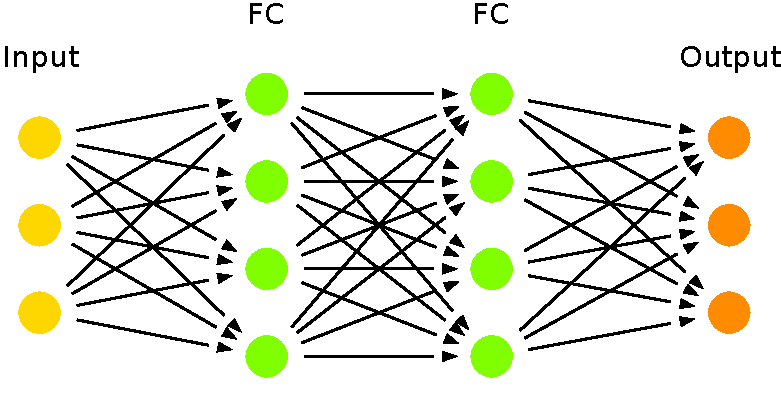
\includegraphics[width=0.9\textwidth]{slike/arch_mlp.pdf}
    \caption{The schematic of the multilayer perceptron architecture}
    \label{fig:MLPArch}
\end{figure}

The $i$-th hidden layer values depend on the values of the previous layer

\begin{equation}
    \vh_i = g_i\left(\mW_i^{\top}\vh_{i-1}+\vb_i \right)
    \label{eq:HiddenLayer}
\end{equation}
and the first hidden layer values depend on the network inputs (i.e., $\vh_0=\vx$). In \cref{eq:HiddenLayer}, $\mW_i$, $\vb_i$, $\vh_i$ are weight matrix, bias vector and layer value of the $i$-th layer, respectively, and $g_i(\cdot)$ is activation function, applied element-wise.

The activation function that is primarily used in state-of-the-art approaches to neural network training is Rectified linear unit (ReLU)

\[
    g(z)=\begin{cases}
    z & z>0\\
    0 & \textrm{otherwise}
    \end{cases}
\]
which has many benefits, including that it is computationally cheap. There are other activation functions, like logistic sigmoid
\[
    g(z)=\sigma(z)=\frac{1}{1+e^{-z}}
    \label{eq:Sigmoid}
\]
and hyperbolic tangent
\[
    g(z)=\tanh(z)
\]

Both of these functions were used as activation functions before the introduction of ReLU. Therefore, these two functions are closely related and only differ in the codomain ($[0, 1]$ vs $[-1, 1]$), while they have the same shape. They are still used today in some applications and particular layers, like LSTM (introduced later).

\subsection{Convolutional neural networks}

Convolutional neural networks are a neural network architecture specialised for processing data that ``use convolution in place of general matrix multiplication in at least one of their layers'' \cite{Goodfellow2016}. They are often used to process grid-like data (1D grid for time series data or 2D pixels for image data). These networks are an extension of the multilayer perceptron, which assumes that neighbouring features are not independent, i.e., they likely belong to the same temporal sequence (in the case of 1D convolution) or the same visual structure (in the case of 2D convolution). Convolutional neural networks are usually deeper than multilayer perceptrons because they are intended for processing more complex data.

The general architecture of convolutional neural networks is illustrated in Figure \ref{fig:ConvArch}. The image illustrates the general convolutional network and its types of layers without specifying whether it is a 1D or 2D convolution. Please note that neurons in the convolution layer are \emph{not} connected to each neuron in the following layer, but only to some of them. As it can also be seen, the convolutional layer(s) are followed by fully connected layers, as in the multilayer perceptron, and the functioning of this type of layer was introduced in Section \ref{sec:MLP}. Two-dimensional convolutional neural networks are left out of this review since they are primarily used for image processing which was not part of this research.

\begin{figure}
    \centering
    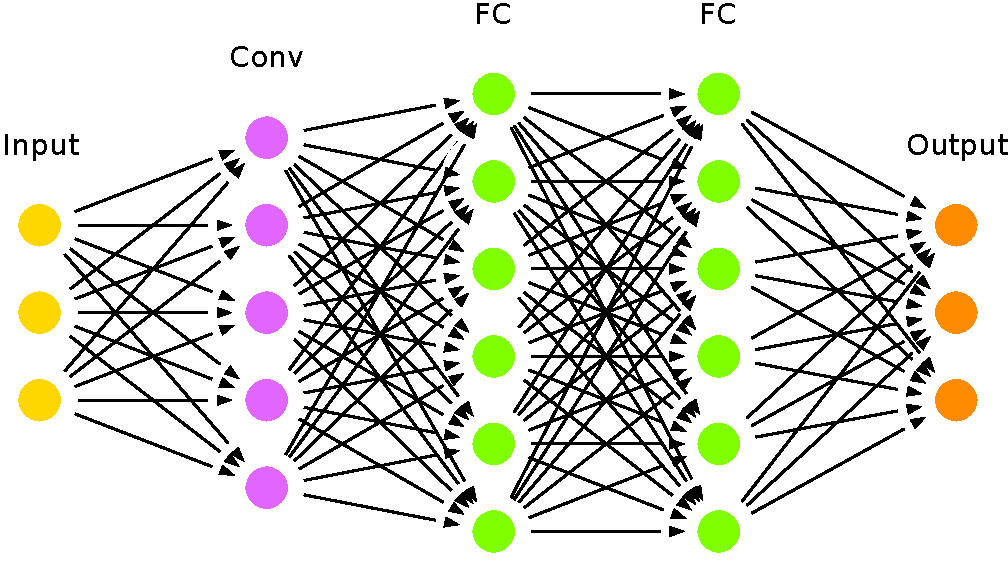
\includegraphics[width=0.8\textwidth]{slike/arch_conv.pdf}
    \caption{The schematic of typical convolutional neural network}
    \label{fig:ConvArch}
\end{figure}

The typical convolutional neural network begins with a convolution layer, usually followed by a pooling layer. After that, more convolution layers may follow, possibly followed by a pooling layer each. Fully connected layers then follow these layers as in the multilayer perceptron case. Stacking the layers enables convolutional networks to learn based on the features extracted by the convolution(s) rather than learning on raw inputs, which is the case of multilayer perceptrons.

The illustration of the one-dimensional convolution operation is shown in Figure \ref{fig:Conv1d}. First, the kernel ``slides'' along the input vector, and the output is a dot product between the ``covered'' part of the input and the kernel, producing a single scalar output. Then, the kernel moves one place right in the input, and the process is repeated until the kernel slides to the end of the input. The example in the figure shows a one-dimensional convolution with a single input sequence, but the example can be easily extended to multiple input sequences (i.e., channels). The same principle can be applied to 2D convolution with images as input, and if that is the case, the kernel will then be a matrix instead of a vector.

\begin{figure}
    \centering
    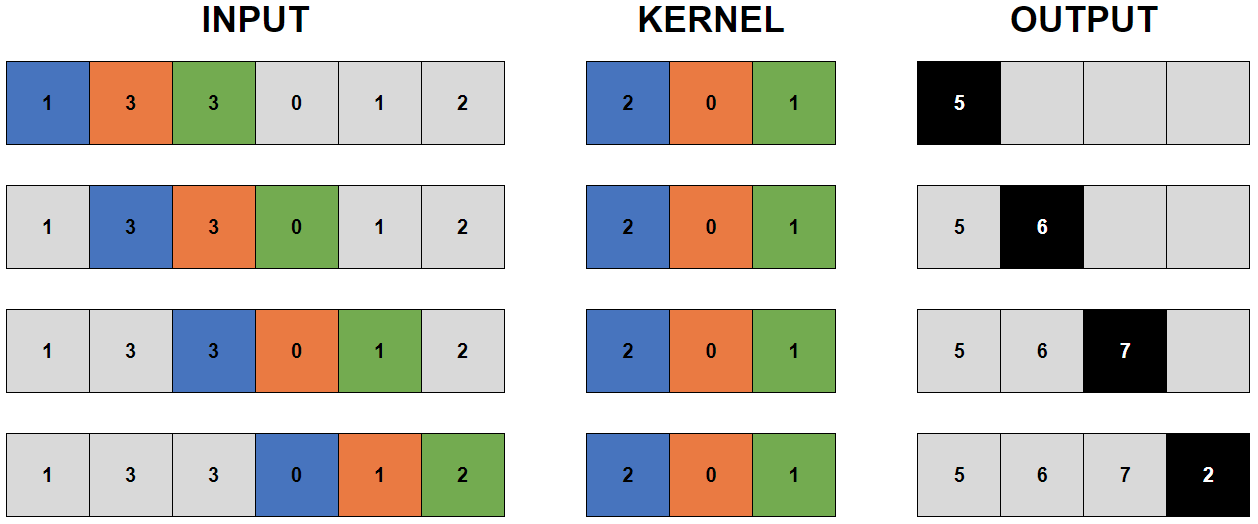
\includegraphics[width=0.9\textwidth]{slike/conv1d.png}
    \caption{The illustration of 1d convolution operation}
    \label{fig:Conv1d}
\end{figure}

One of the main characteristics of convolution layers is sparse weights, meaning that, unlike in multilayer perceptrons, not necessarily every unit is connected to all units in the next layer. This kind of connection is achieved because the kernel used in the convolution operation is smaller than the input, as is evident from the example in Figure \ref{fig:Conv1d}. Finally, the results of the convolution operation are activated using the activation function, most commonly ReLU.

Pooling layers may be used, but they are not mandatory in convolutional neural networks. The idea of a pooling layer is to reduce the dimension of the features produced by a convolutional layer. It takes the activated outputs of a convolutional layer and produces an output at a location that is a summary statistics about the location's surroundings (maximal or average values are the most used summary statistics in pooling layers), as shown in \cref{fig:Pooling}. The pooling works by applying a sliding window of a specific size (smaller than the convolutional layer output). As a convolution operation might be viewed as one that extracts features from raw data, the pooling operation may keep the ``strongest'' or average feature among those extracted, using max pooling and average pooling, respectively. This way, downsampling of the signal is achieved. Thus, the answer to whether the pooling layer should be used or not depends on if downsampling is desired. Please note that in networks with multiple convolutional layers, a pooling layer does not have to be added for each of the convolution layers.

\begin{figure}
    \centering
    \subfloat[Max pooling]{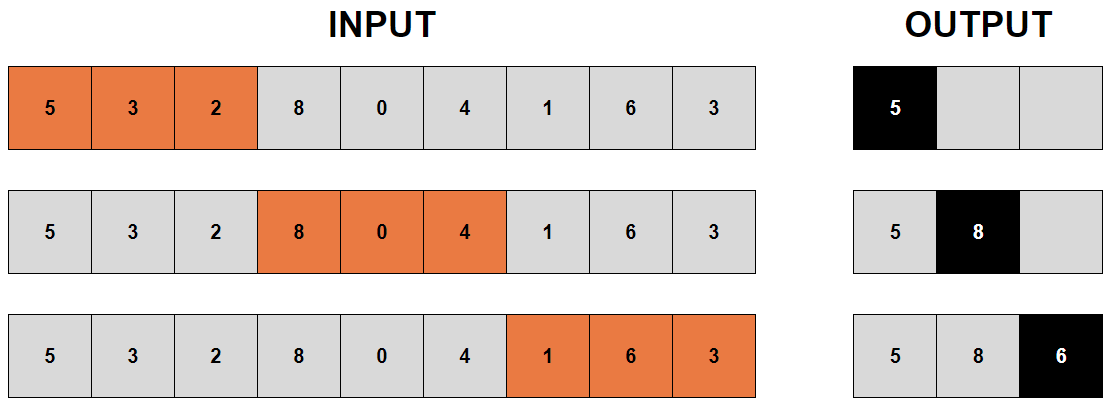
\includegraphics[height=4cm]{slike/pooling_max.png}}
    \vfill
    \subfloat[Average pooling]{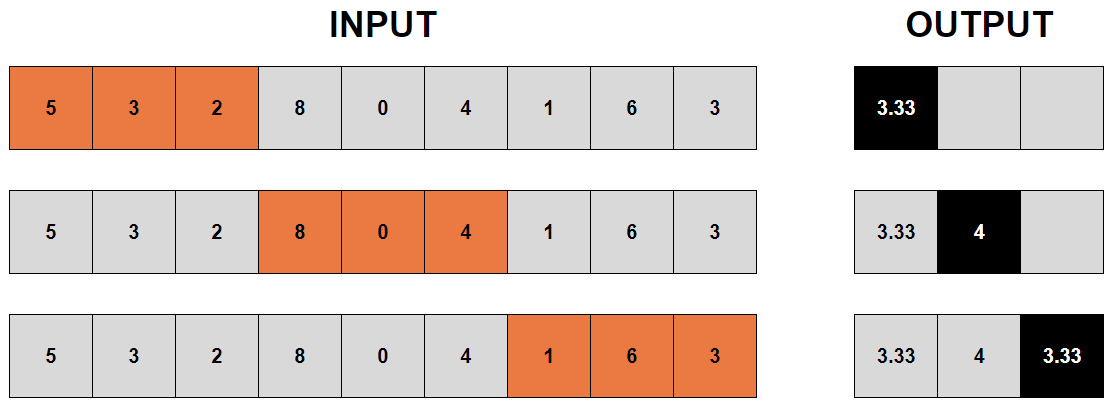
\includegraphics[height=4cm]{slike/pooling_avg.png}}
    \caption{The illustration of different types of pooling operation}
    \label{fig:Pooling}
\end{figure}

\subsection{Recurrent neural networks}

Recurrent neural networks (RNN) are used to process sequential data, most often temporal sequences. Most notable applications include signal processing and natural language processing. A recurrent neural network contains one or more recurrent layers at the beginning of the network, with fully connected layers following. It is similar to 1D convolutional neural networks in that both have a similar structure, but significant differences exist in how the data are processed in convolutional and recurrent layers.

The recurrent layer consists of \emph{cells} that feature a loop (or feedback), which makes a piece of information possible to persist between the training steps. This way, a recurrent neural network may be seen as multiple copies of the same network chained one after another. However, these networks are unable to handle ``long term dependencies'' \cite{Bengio1994} (finding the connection between previously seen information and the present task). Therefore, long Short Term Memory (LSTM) networks are introduced \cite{Hochreiter1997} to resolve this problem. This architecture came as a replacement to traditional recurrent neural networks and are nowadays used for most applications.

\begin{figure}
    \centering
    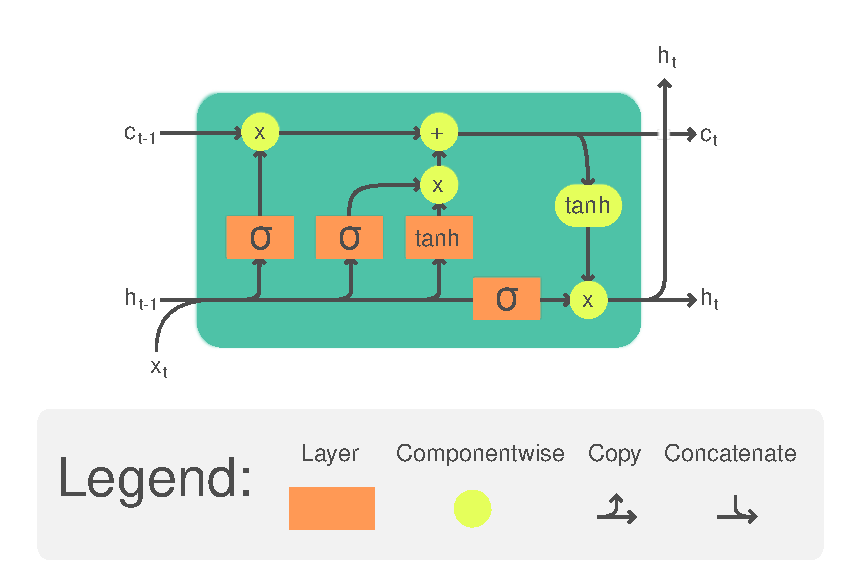
\includegraphics[width=0.8\textwidth]{slike/LSTM_Cell.pdf}
    \caption[LSTM Cell]{\href{https://commons.wikimedia.org/wiki/File:LSTM_Cell.svg}{LSTM Cell} \copyright\,Guillaume Chevalier CC-BY-SA 4.0}
    \label{fig:LSTMCell}
\end{figure}

The LSTM cell is somewhat different from the classical RNN cell because its default behaviour is to learn long-term dependencies. A schematic of the LSTM cell is shown in Figure \ref{fig:LSTMCell}, where it can be seen that it contains four layers, of which three are activated with sigmoid activation and one with hyperbolic tangent activation (instead of one in classical RNN), that interact with the data. Furthermore, it has a state, which can be controlled using gates (horizontal line on top of the schematic in Figure \ref{fig:LSTMCell}, with input $c_{t-1}$ and output $c_t$). This way, the cell can decide whether a piece of information will be kept or discarded. More detailed insights into how LSTM cells work, along with the mathematical details, can be found in \cite{Olah2015}.

\section{Autonomous Mobile Robot Navigation}

Autonomous mobile robots are increasingly being used in dynamic (changing) environments \cite{Kunze2018,Guiochet2017,Ramachandram2017,BoninFont2008,Jarvis2008}. Due to the uncertain nature of such environments, robot behaviour should be adaptive to operate adequately with minimal or no human-operator effort. These environments range from air-, water- and ground-based ones to space-based ones \cite{Kunze2018,BoninFont2008}. This dissertation focuses on ground-based autonomous mobile robots. Thus, the term \emph{autonomous mobile robots} will refer to ground-based mobile platforms for this dissertation. However, some of its contributions and conclusions could easily be extended to other domains (like air and water).

In order to move in the environment, mobile robots need to be equipped with appropriate navigation methods. Traditionally, navigation is usually a combination of three fundamental operations: localisation, path planning and mapping (and map comprehension). Localisation aims to estimate the current robot state (i.e., pose) based on sensor readings, a probabilistic procedure due to the dynamic environment. Thus, localisation provides a probability distribution that the robot is in a certain state (pose). State-of-the-art localisation methods are based either on Extended Kalman Filter \cite{Jetto1999,Moore2015} (and its variants) or Monte Carlo Localisation \cite{Dellaert1999,Thrun2006}. The mapping is usually done using a procedure called Simultaneous Localisation and Mapping (SLAM) \cite{Leonard1991,DurrantWhyte2006}. It is a process in which the environment map is constructed from sensor data and simultaneously used to estimate the robot's location relative to the created map. There exist SLAM implementations based on both Extended Kalman Filter \cite{Dissanayake2001,Leonard2000,Guivant2001}, (called EKF-SLAM) and Monte Carlo Localisation \cite{Montemerlo2002,Montemerlo2003} (called FastSLAM).

When the map is available, the navigation is termed as \emph{navigation in a known environment}. The navigation stack usually consists of two fundamental components. The first component is called global planner, and it has access to the map and needs to find a collision-free trajectory (path) to the given goal. For that purpose, usually, graph-based algorithms are used, most often Dijkstra \cite{Dijkstra1959}, or A$^*$ \cite{Hart1968}, which are both \emph{de facto} standard even today, besides the fact that they were published some 50 years ago. The other component is called the local planner, which does not have access to the map, but has access to the sensor data and the trajectory part in the robot surrounding. It is used to avoid dynamic obstacles\footnote{Dynamic obstacles are those that are not part of the environment, i.e., they are not visible on the map. They can be either moving or non-moving obstacles}. Although this component is named local planner, it does not strictly need a plan since the obstacle avoidance may be implemented reactively (only based on present sensor data). Many algorithms may be used for obstacle avoidance within this framework \cite{Khatib1985,Minguez2005,Fox1999,Borenstein1991,Fiorini1998}. These two components work together to move the robot to the given goal avoiding dynamic obstacles on the way.

When considering the application of autonomous mobile robots, long-term autonomy and safety are of primary interest \cite{Kunze2018}, especially if there is human-robot interaction or cooperation in the application scenario. This fact has been highlighted by several recent EU-, USA-, and Japan-based projects that consider safety as the main challenge in human-robot interaction\cite{Guiochet2017}. In order to alleviate these concerns, researchers usually provide a robot with an appropriate form of artificial intelligence. The current state-of-the-art approaches use some form of Deep Neural Network \cite{Sze2017} in conjunction with a fusion of data from several sources, which is referred to as \emph{deep multimodal learning} \cite{Ramachandram2017}. While the deep multimodal learning approach has found many exciting applications within recognition and classification fields (e.g. in text recognition  \cite{Wang2017}), applications to autonomous robot navigation are relatively rare (but do exist, e.g. in \cite{Zhu2017,Giusti2016,Ran2017}). However, deep multimodal learning has been successfully used in the field of semi-autonomous cars \cite{Ramachandram2017,Chen2015,Jain2016} which also have well-known and large databases available for testing and benchmarking new approaches \cite{Geiger2013,Maddern2016}. 

The data fusion itself can be achieved on three levels\cite{Ramachandram2017,Toprak2017}: feature level (sometimes referred to as \emph{early fusion} or \emph{pre-mapping fusion}), decision level (sometimes referred to as \emph{late fusion} or \emph{post-mapping fusion}) and mid-level (sometimes referred to as \emph{intermediate fusion} or \emph{midst-mapping fusion}). Some variations exist within each of these high-level fusion architectures (e.g. in \cite{Chou2018}). Regardless of which fusion scheme is used, ``\emph{most multimodal deep-learning architectures proposed to date are meticulously handcrafted}'' \cite{Ramachandram2017}. A minor modification to the neural network task usually requires retraining the whole network or training it from scratch. This procedure is time-consuming and computationally expensive (especially in multimodal networks) since neural networks are designed to do one specific task for which they require an abundance of training data (usually images/videos) \cite{Ahmad2005}.

State-of-the-art approaches mostly use neural networks to tackle intelligent robot control. Thus, they will be the focus of the remainder of the review. First, an overview of data collection methods will be given, followed by the applications of neural networks in the field of autonomous mobile robots. Finally, since this dissertation focuses on autonomous mobile robot navigation, it will be given a particular emphasis.

\subsection{Data collection}

Neural networks need large and diverse datasets for training, the collection of which is a time-consuming and labour-intensive task and one which usually requires human operator supervision \cite{Giusti2016,Gandhi2017,Pinto2016}. Thus, it becomes a bottleneck of the whole method development process, regardless of the task. Several different approaches to tackling the issue have been proposed in the literature, but they all, in general, take a significant amount of time and resources and pose a particular risk of damage to the robot and surroundings \cite{Gandhi2017,Pinto2016}. Moreover, in some instances, they rely on additional algorithms, such as various forms of deep reinforcement learning \cite{Mnih2015,Xie2017}.

Another issue that arises while collecting data by operating a real-world robot that is efficiently circumvented by using simulation is that human operators tend not to collide with objects in the environment, thus limiting the number of negative examples and consequently algorithm's performance. It is especially emphasised when collecting data for training neural networks for obstacle avoidance since it drastically limits the existence of negative samples, which are crucial for good performance.

On the other hand, the simulation makes running extensive and elaborate experiments efficiently while providing necessary data in a safe and controlled manner, as in some works \cite{Chen2015,Gupta2017,Mirowski2016} where the training and testing were achieved in the simulation environment only. However, an issue is that training the networks on synthetic images generated in simulation does not necessarily guarantee good real-world performance due to the \emph{simulation-to-reality gap} \cite{Bousmalis2017,Bousmalis2018}, which may be defined as the difficulty in transferring simulated experience into the real world \cite{Bousmalis2018}. Neural networks trained with such data usually need to be retrained with additional real-world examples \cite{Gandhi2017}, thus lengthening and complicating the deployment process.

There have been various approaches to overcoming the gap. In \cite{Bousmalis2018}, for vision-based grasping, training data was collected in simulation and presented a very challenging problem of transferring obtained data to the real world. In \cite{Xie2017}, deep reinforcement learning was used with synthetic images to train obstacle avoidance for mobile robots and claimed to have achieved high performance using the proposed approach. Some approaches have recently been proposed using simulation data for training \cite{Bousmalis2018,Zhu2017}, but there, a human supervisor may still be needed, and more complex networks are used. In \cite{Zhu2017}, an approach to training vision-based navigation (flight) in simulation using only synthetic images (i.e., without a single real-world image). It is reported that highly randomising rendering settings can train a policy that generalises appropriately in the real world for synthetic images. In \cite{Koenig2004}, some issues of deep reinforcement learning-based approaches are resolved by using simulation environments for collecting training data for visual navigation. The proposed method generalises appropriately and can be transferred to a real robot with a little fine-tuning.

Recently some works have emerged where testing of convolutional neural networks trained with the data from the simulation was conducted in real environments with no or little retraining \cite{Zhu2017,Sadeghi2016}. The use of simulation for such tasks is mainly possible due to recent advances in computer graphics, which makes possible a rich and vivid representation of real-world environments and their physics, thus narrowing the before-mentioned gap. However, another more recent approach is to use a combination of photo-realistic data in conjunction with non-photo-realistic domain randomised data to leverage the strengths of both \cite{Tremblay2018}. This approach was then used to learn the object 3D pose from RGB images, outperforming state-of-the-art neural networks trained on natural images.

The majority of available literature uses RGB cameras as a primary source for collecting data, and some form of deep learning is used to interpret the scene captured by a robot-mounted camera and infer control actions \cite{Sullivan2017,Hadsell2009,Giusti2016,Tai2016,Gandhi2017,Liu2017}. LiDAR-based ones also exist \cite{Maturana2015}, but in significantly lower numbers and not for ground-based mobile robot obstacle avoidance. While images are inherently information-rich, they do not possess depth information and use significant computational resources. Of course, depth cameras (like Microsoft Kinect and Intel RealSense) can be used to avoid the issue \cite{Tai2016,Correa2012}, but this is then a completely different approach, and one better tackled by 2D/3D LiDAR \cite{Bousmalis2018}.

The research presented in this dissertation was partly motivated by \cite{Gandhi2017} in which an unmanned aerial vehicle was used to collect data for training a deep neural network by randomly crashing it (10,000 times) into objects within the real-world environment. That work is based on camera data and conducted in the real world. However,  the method for data collection in this research is based on simpler LiDAR data and data were collected simulation, making it safer for both the robot and its surroundings and enabling the collection of an abundance of training data. Furthermore, the simulation-to-reality gap is bridged by using simple data and straightforward metrics (distance). Thus, the difference between simulation and reality should be reduced, leading to better performance in the real world.

\subsection{Neural network-based autonomous navigation}

Neural networks have been used to learn control policies in end-to-end fashion \cite{Levine2015, Muller2006}. In \cite{Levine2015} it was examined if end-to-end training of both the visual and the control system provided better performance than in the case when they were trained separately. These policies were represented by deep convolutional neural networks with a supervised learning approach via guided policy search. While the paper mainly deals with applying visuomotor policies on robot manipulator tasks (e.g., screwing a cap onto a bottle, placing a coat hanger on a rack), some of its conclusions can be transferred to a mobile robot domain. One such conclusion is that the end-to-end approach outperformed the approach in which the vision layer was trained separately. Although some drawbacks associated with generalisation and visual distractors were noted, the authors suggest straightforward ways of dealing with them. In \cite{Muller2006} an end-to-end approach was also used with steering angles obtained by processing raw input images. It was achieved using a convolutional neural network with six layers, trained in a supervised manner using data obtained from a human operator in the real world in various weather conditions and terrains. The training set consisted of 95,000 image pairs (since two cameras were used). The authors reported good navigation and obstacle avoidance capabilities even at speeds of 2 m/s and noted that the proposed approach eliminates the need for any form of calibration and parameter tuning and the need to select features from raw images. It is worth noting that end-to-end control policies are also finding their way into the field of autonomous cars \cite{Bojarski2016} where additional, domain-specific problems exist, which can also be addressed by deep neural networks or recurrent neural networks, like negotiating safe driving \cite{ShalevShwartz2016} or anticipating (and correcting) human actions \cite{Jain2016}.

The works in the area of autonomous navigation tackle different aspects of navigation using deep neural networks \cite{Zhu2017,Chen2015,ShalevShwartz2016,Hadsell2009,Gupta2017}. In \cite{Hadsell2009} the authors did not use an end-to-end approach but developed a long-range vision system based on deep neural networks, which interacted with path planning and obstacle avoidance algorithms to generate steering commands. The long-range vision module was trained in real-time in a self-supervised manner, with the stereo supervisor taking care that data and labels are not changed. The supervisor involved several algorithms (like ground plane estimation and statistical false obstacle filtering) which interacted in a complex manner. The long-range classifier demonstrated obstacle detection capabilities from 5 to over 100 meters. The approach was tested in two separate scenarios. First, the classification network was tested as a standalone system where different network architectures were applied. It was shown that the hybrid unsupervised/supervised approach performs the best (with error rates of about 8\%). After that, the neural network was tested as a part of the navigation system. It ran at 1-2 Hz, enabling strategic navigation from 5 m to the goal (also, a short-range algorithm runs in parallel at 8-10 Hz to avoid obstacles). The testing was conducted on several courses where a long-range module proved helpful and enabled error- and intervention-free navigation. The improvement was also evident in the total time and distance taken to reach the goal.

In \cite{Gupta2017} a first-person view visual-based system was also used, but for an indoor environment and in an end-to-end manner. Here, a complex structure of several neural networks was used to map the space and navigate through it. Used neural networks were of convolutional type (ResNet-50 pre-trained on ImageNet). The process is a reminiscence of Simultaneous Localisation and Mapping (SLAM), but the authors note that their approach differs in several ways from classical approaches, one being that it can learn statistical regularities of the environment. Thus, the approach enables tracking of visited parts of the environments as well as semantically driven navigation (e.g., ``\emph{go to a table}''). The proposed approach was developed in the simulated environment, based on Stanford large-scale 3D Indoor Spaces (S3DIS) dataset obtained by 3D scanning six large-scale indoor spaces within three different buildings. Obtained results demonstrated that the proposed approach outperforms classical approaches such as reactive strategy and standard memory-based architectures (e.g. LSTM).

In \cite{Zhu2017} the authors used a deep siamese actor-critic model within the deep reinforcement learning framework for target-driven visual navigation. The developed model was given an RGB image of the current scene and an additional RGB image of the target, providing the necessary action: moving forward, moving backwards, turning left, and turning right. The authors highlight that in this manner, their reinforcement learning approach becomes more flexible to changes in task goals (in contrast to more standard approaches like  \cite{Mnih2015} in which the goal is hardcoded in the neural network). In order to achieve this, the authors developed a custom 3D simulation framework named AI2-THOR (The House Of inteRaction) by providing reference images to artists, which then created realistic 3D environments (32 scenes in total). The approach was tested both in simulation and in the real environment with SCITOS mobile robot. Obtained results from simulation showed shorter average trajectory length for the proposed approach when compared to the baseline methods, while results from real-world experiments demonstrated that the networks trained in simulation and fine-tuned on real data converged faster than networks trained from scratch. Authors especially emphasise that their approach is generalisable to new scenes and new targets.

In \cite{Sadeghi2016} the authors went a bit further, developing a neural network-based model solely in simulation and applying it in the real world without any modification or additional training. It was used to search for a control policy that can process raw data (e.g. images) and output control signals (velocity), which relied on reinforcement learning. Since, as the authors outlined, reinforcement learning needs at least some collisions (negative examples) during training, it can be a challenging and risky undertaking to train a mobile robot on real-world data. To avoid real-world training, the authors used Blender \cite{Blender2018} to construct several corridor-based environments (24 using 12 different floor plans) for the generation data used for training a deep, fully convolutional neural network with dilation operations, built on VGG16 architecture \cite{Simonyan2014}. It is interesting that authors intentionally rendered environments with a lower degree of realism or visual fidelity and ones with randomised textures, lighting conditions and obstacle placement and orientation, based on the hypothesis that generating a large number of such environments with numerous variations (of textures of which there were 200) would produce a model which generalises well. This hypothesis was verified in experiments both in synthetic and real environments. The simulation-based testing showed that the proposed reinforcement learning approach outperforms the used baseline methods (Straight controller and left, right and straight -- LRS -- controller), but in real-world testing, experience some collisions. The obtained results led the authors to conclude that the proposed approach is viable and that further testing is needed, such as including additional sensors (like RGB-D cameras). A similar approach that employs a reinforcement learning-based approach for control policy search can also be found in \cite{Zhang2015}.

It is worth noting that the implementation of ensembles of neural networks is not a new idea. In \cite{Hansen1990} they were used in conjunction with a plurality consensus scheme for classification applications, with a focus on optimising neural network parameters and architectures. The approach was tested in two (simple) scenarios: generalised exclusive disjunction (XOR) operator and region classification in the 20-dimensional hypercube. While the obtained results improved over single copy networks, they apply only to neural networks (i.e., no other algorithm can be introduced into the approach). There have also been approaches that utilise a single deep neural network for object detection, decision making and inferring control commands \cite{Tai2017}, inspired by the way a human brain works. While this work focuses on robotic applications (using RGB-D cameras as primary sensors) and presents promising real-world results for indoor robot exploration tasks (including obstacle avoidance), it has some potential drawbacks. The approach \cite{Tai2017} is intended only for neural network-based strategies, and since it uses convolutional neural networks, it requires large amounts of data for training (which were recorded with human drivers exploring an environment).

Additionally, the use of fuzzy logic variants (e.g., fuzzy integral) for fusing outputs from several neural networks has also been proposed before in \cite{Cho1995} (for dynamic nonlinear process modelling) and \cite{Ahmad2005} (for robust character classification purposes). However, in \cite{Ahmad2005} non-adaptive fusion mechanism was used (i.e. the contribution of each network was known in advance based on its loss function). This approach is not suitable for the intended application, where different controllers can have variable importance due to the dynamic nature of the environment. In addition, the approach (as is the case in \cite{Cho1995}) does not consider a way to include other types of controllers (besides neural networks) or human input. Some work has been done on adapting the fusion scheme, like in \cite{Jacobs1991} but without the use of fuzzy-based logic, using a gating network that makes a stochastic one-out-of-n decision about which single network to use for a particular instance. The approach was tested in a multispeaker vowel recognition task. In addition, as can be seen from the above discussion, the primary intended application is not related to robotics in many such examples.

In \cite{Pfeiffer2017}, an end-to-end motion planning for mobile robots was implemented. A Convolutional Neural Network (CNN) was trained (in a supervised manner) using simulated sensor data gathered in \emph{Stage 2D} environment \cite{Vaughan2008}. The term \emph{end-to-end control} refers to the fact that the input data was directly mapped to the steering commands\footnote{The steering commands consist of the translation and rotation components}. The training data was recorded while navigating in a simulation on a known map using Robot Operating System (ROS) \cite{Quigley2009} \emph{2D Navigation stack} with its local planner based on Dynamic Window Approach -- DWA \cite{Fox1997} and global planner based on Dijkstra algorithm \cite{Dijkstra1959}. However, when testing was done (both in a simulation environment and in the real world using Kobuki based Turtlebot), no map was given to the robot but only the relative distance to the target. Thus, in essence, the CNN was applying the navigation strategies learnt during training. The approach showed promising results, being able to navigate to the desired location in the real world without the need for a map while avoiding moving obstacles (although testing was limited). However, the authors outlined several situations where the control algorithm needs some help to get out of situations that neural networks cannot handle properly: large open spaces and convex dead-end regions. Furthermore, the incidence rate of human assistance dropped if additional fully connected layers were added (this was not true for simulation-based environments).

It should be noted that work from \cite{Pfeiffer2017} has some similarities to the research given in this dissertation: using 2D LiDAR (Light Detection and Ranging) data instead of a video stream for the training of neural networks, using simulation as a source of data for self-supervised learning and navigating without the need for a map. However, this approach achieves those goals differently within the framework, which seems more flexible and can integrate additional (standard) control algorithms. It also uses both positive and negative examples for training. For example, successful obstacle avoidance is regarded as a positive example, while the crash is considered a negative example in the process.

Obstacle avoidance is one of the tasks that is needed for autonomous mobile robot navigation \cite{Sullivan2017}. Due to the uniqueness of different environments, it is usually not convenient or even possible to tailor-made obstacle avoidance algorithms for every conceivable situation and environment. Thus, there is a need for a more general approach to the problem. In recent years, the reemergence of neural network-based algorithms has led to some exciting applications in mobile robotics. For example, in \cite{Hadsell2009}, neural networks were used for feature extraction from stereo images, as a part of a complex system for long-range vision used in the navigation of autonomous off-road vehicles (robots), while in \cite{Giusti2016}, neural networks were used to infer control action that will keep the robot on the forest trail. In \cite{Tai2016}, authors demonstrated the effectiveness of a neural network-based model-less obstacle avoidance algorithm in an indoor environment. In \cite{Yada2021}, obstacle avoidance was achieved using laboratory-grown biological neurons in such a way that neurons were stimulated when the robot went the wrong way or collided with an obstacle. This way, the robot learned to get back on the way to the given goal.

\section{Robotic Manipulator Interaction Force Estimation}

Most often, robotic manipulators are programmed to (repeatedly) execute a set of predefined trajectories (commonly referred to as \emph{position control}).  However, the use of predefined trajectories is inconvenient in situations where data on the position (or configuration) of the robotic manipulator alone does not guarantee the successful execution of the given task (e.g., when the object to be grasped by the robot does not always come in the same known orientation). In such situations, it is necessary to use \emph{force control}, which can also be considered as \emph{interaction control} \cite{Siciliano1999}. In such scenarios, forces and torques are used to detect and measure the interaction, and force-torque sensors are used for that task. This robot control method is often most suitable for the actions of robotic manipulators involving physical contact between the robot and its environment, as well as in the collaboration and interaction of the robot and the human. However, pure force control is of little use when the robot moves in the free space (not interacting with the environment). Thus, a combination of force control and position control is often used to overcome this deficiency. Moreover, when using haptic force feedback interfaces to control or interact with a robot, contact force information is necessary for the haptic interface to work and for the human operator to receive feedback on the interaction with the robot \cite{Song2019}.

In most application scenarios, a force-torque sensor is mounted at the robot's tip, i.e., the robotic arm's wrist. However, if low-payload manipulators are used\footnote{This is a relatively common case with manipulators intended for education, while is generally not the case with robotic manipulators intended for applications in the industry}, placing a force sensor at the tip of the manipulator may be inconvenient or even impossible. This disadvantage can be circumvented by using methods to estimate the forces instead of direct measurements using sensors. The estimated forces can also be combined with force measurements, a good example being able to ``\emph{distinguish the effects of inertial forces due to acceleration of a heavy tool from contact forces with the environment, as both these forces would show up in the measurements from a force sensor located at the robot wrist}'' \cite{Alcocer2003}.

With the kinematics known, the force acting on the end-effector may be expressed as 
\[
    \mF = \mJ^\top(\vq)\vtau
\]
where $\vtau$ are forces/torques expressed in generalised coordinates (as well as the control variable in the case of the force control scheme is used), $\mJ(\vq)$ is robot end-effector Jacobian (which is a function of the robot state $\vq$), and $\mF$ are forces and torques acting on the end-effector. However, this method requires that joint-side forces or torques are measured. The joint-side forces and torques are usually measured internally and provided by the robot controller but are available depending on which robot is used since not all robots have this feature. Furthermore, the robot kinematics is not always fully known or, when it is known, it includes errors due to noisy sensor readings. Thus, force estimation methods may be applied to obtain accurate force and torque estimates. 

One commonly used method for estimating forces is based on force observers. The estimation of forces acting on a body is performed from the measured position and orientation data with the knowledge of control forces and torques \cite{Hacksel1994,Ohishi1991,Eom1998,Alcocer2003,Stolt2012}.

An observer-based method for estimating external forces (or environmental forces) acting on a robotic manipulator is proposed and experimentally tested in \cite{Hacksel1994}. The method uses the knowledge of body position and orientation and control forces (torques) in a force control scheme and models the observer error as a damped spring-mass system driven by force (torque). However, it was shown that an accurate dynamic model of the robot is needed for accurate estimates. In \cite{Alcocer2003}, a generalisation of the force estimation method based on observers proposed in \cite{Hacksel1994} is proposed. The paper presented two versions of the observer: linear and nonlinear, the latter experimentally verified on a real-world robotic manipulator. In \cite{Stolt2012} the force is estimated from the control error, which is, in turn, based on the detuning of the low-level joint control loop.

The methods based on the observers are pretty old (from the 1990s) but still used today, and some of them are extended and are using neural networks to tackle some issues and improve performance. For example, in \cite{Liu2021} a simple multilayer perceptron neural network with a single hidden layer is used to model friction to obtain better force estimates, given a robot subject to model uncertainty. Besides the simple ones, more complex neural networks were also used \cite{Dine2020}, where a recurrent neural network was used to model the disturbance observer, to remove non-contact forces appearing due to robot motion from the estimate.

In \cite{Damme2011}, the forces are estimated using two proposed methods, both based on actuator torque measurements (i.e., link-side joint torques of a robotic manipulator). The first method is based on the filtered equations of robot dynamics and the recursive least-squares estimation algorithm, while the other method produces force (torque) estimates using a generalised momentum-based observer. The results obtained in the experiments using these methods showed that outputs of the two algorithms agree very well, and it was concluded that despite the different origins of the proposed methods, both estimators' performances were good. However, as reported in the paper, the observer-based method performs better when a fast response is needed. Furthermore, if joint motor torques are not available, they could be estimated by measuring the electric current through each motor, allowing the forces at the robotic manipulator tip to be estimated (indirectly) from the motor currents, as in \cite{Wahrburg2018}.

Deep neural network architectures were applied in robotics to the problems of grasping \cite{Levine2017}, control \cite{Jin2018}, domain adaptation \cite{Bousmalis2018} and the like. However, the estimation of forces in robotics using deep learning has been somewhat less researched, but there is still research on the subject. In \cite{Smith2005}, neural networks are used as an extension of the force observer that requires explicit and exact knowledge of the dynamic model of a robotic manipulator. If the dynamic model of a robotic manipulator is very complex, insufficiently known, or insufficiently accurate, this leads to unsatisfactory force estimation results. The authors suggest the use of neural networks for the inverse dynamics of a robotic manipulator. They argue that the proposed model is more accurate than using force observers themselves and that it is easier to implement since it is not necessary to know the dynamic model of a robotic manipulator. There are also approaches for specific applications, for example, in robotic surgery \cite{Marban2019,Aviles2015}, where force estimation is done without force sensors, using some kind of visual feedback and neural networks.

In recent years, methods based on neural networks that can learn robots' (inverse) dynamic models have been developed. These methods have in common that they learn and simultaneously include the prior knowledge of the system that is being modelled. For physical systems (the robot is a physical system), the prior knowledge is formulated as physical laws (law of energy conservation), introducing additional constraints leading to better performance when incorporated into a neural network.

In \cite{Lutter2019, Lutter2019a}, the authors emphasise that deep learning has achieved impressive success in all fields of use, except physical systems. For that reason, a novel model that uses prior knowledge of the system is modelled using deep learning, termed Deep Lagrangian Network (DeLaN). This knowledge (physics) of the systems involved is incorporated into deep neural network architectures. For that purpose, the Euler-Lagrange equation is used before obtaining more accurate models and ensuring physical plausibility while assuring that the models can extrapolate new samples (an example would be following the identical trajectories at different velocities). On the other hand, Multilayer perceptrons occasionally show overfitting to training data and thus, in these cases, need a lot more training data to generalise appropriately and are not guaranteed to obey the energy conservation law. Solving the Euler-Lagrange equation yields
\[
    \mH(\vq)\ddot{\vq} + \vc(\vq,\dot{\vq}) + \vg(\vq) = \vtau
\]
where $\mH$ is the mass matrix, $\vc$ is centripetal and Coriolis forces, $\vg$ is the gravity term, and $\vtau$ is the vector of control inputs (in case of robotics, these are joint-side torques. This equation is implemented as a network shown in Figure \ref{fig:DeLaN}. During the training, the gradients are backpropagated through all blocks marked with orange colour.

\begin{figure}
    \centering
    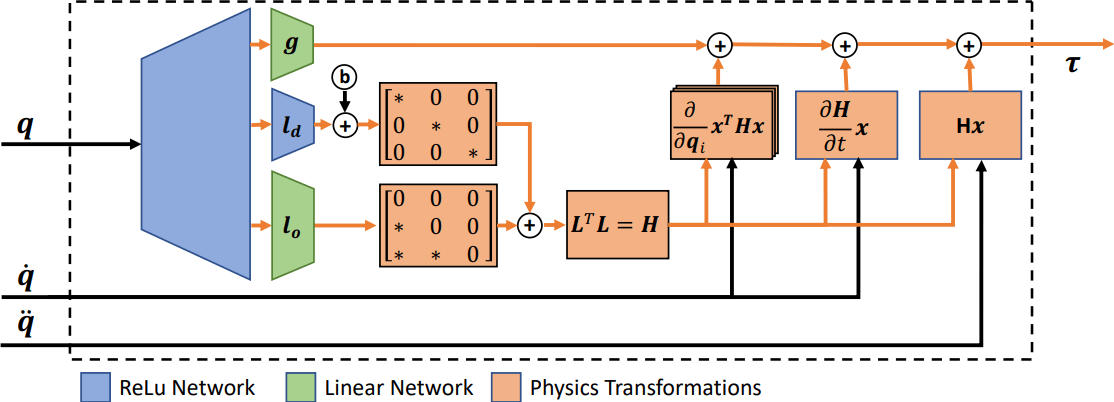
\includegraphics[width=0.9\textwidth]{slike/delan.png}
    \caption[DeLaN network architecture]{DeLaN network architecture \cite{Lutter2019}}
    \label{fig:DeLaN}
\end{figure}

A similar but more general method for learning arbitrary Lagrangians called Lagrangian Neural Networks (LNN) was presented in \cite{Cranmer2020}. Along with it, a good overview of neural network-based models for physical dynamics is given in the paper. It is shown that the complex model obtained by this approach successfully complies with the law of energy conservation, as is illustrated in \cref{fig:LagrangianNN}. Furthermore, the obtained results show that the use of LNN almost strictly conserved the energy, unlike the baseline. The results were also compared to those obtained in \cite{Greydanus2019}, an approach inspired by Hamiltonian mechanics and showing similar performance, except that LNN can learn from arbitrary coordinates, while the method proposed in \cite{Greydanus2019} can only learn using canonical coordinates.

\begin{figure}
    \centering
    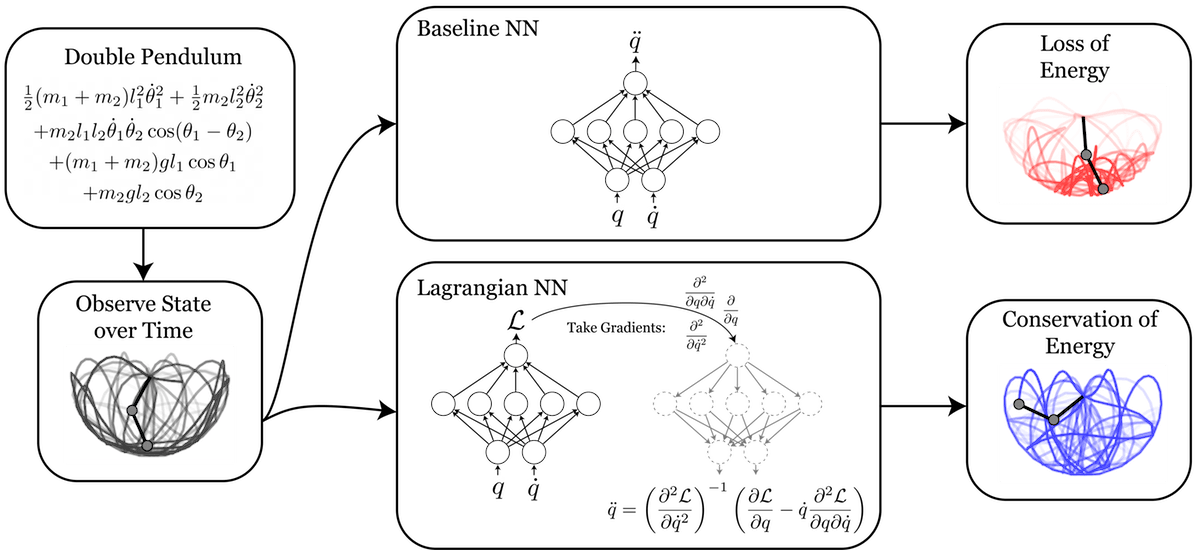
\includegraphics[width=0.9\textwidth]{slike/lnn.png}
    \caption[Lagrangian neural network]{Lagrangian neural network -- comparison with MLP for the example of double pendulum \cite{Cranmer2020}}
    \label{fig:LagrangianNN}
\end{figure}

In \cite{Ledezma2017}, an approach called First-order Principles Network (FOPnet, \cref{fig:FOP}) was presented, which differs from classical neural networks for which the architecture is usually identified by trial and error. However, in the proposed approach, the network topology is determined from the physical characteristics of the dynamic system being modelled. Thus, this approach makes the topology (architecture) not subjective but dictated by the physics of the dynamic system. It was demonstrated how FOPnet for a robotic manipulator emerged from the Newton-Euler formulation for representing robot inverse dynamics. It showed that networks that compute dynamics and kinematics have weights that correspond to inertial and DH parameters of the robot.

\begin{figure}
    \centering
    \subfloat[FOPnet construction]{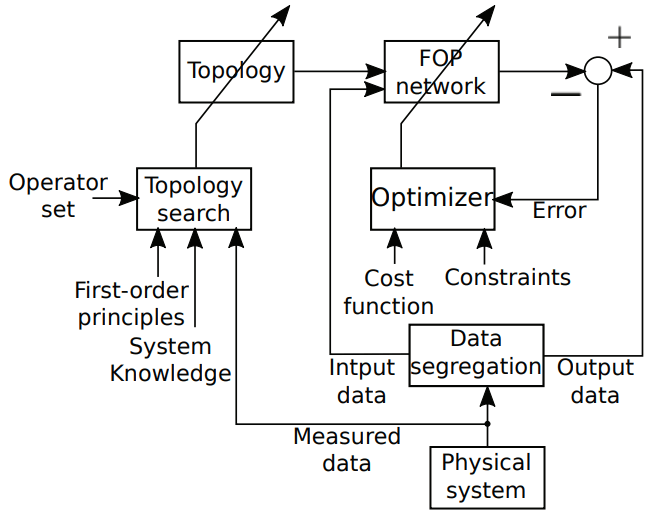
\includegraphics[width=0.495\textwidth]{slike/FOP1.png}}
    \hfill
    \subfloat[FOPnet for an N-DoF manipulator]{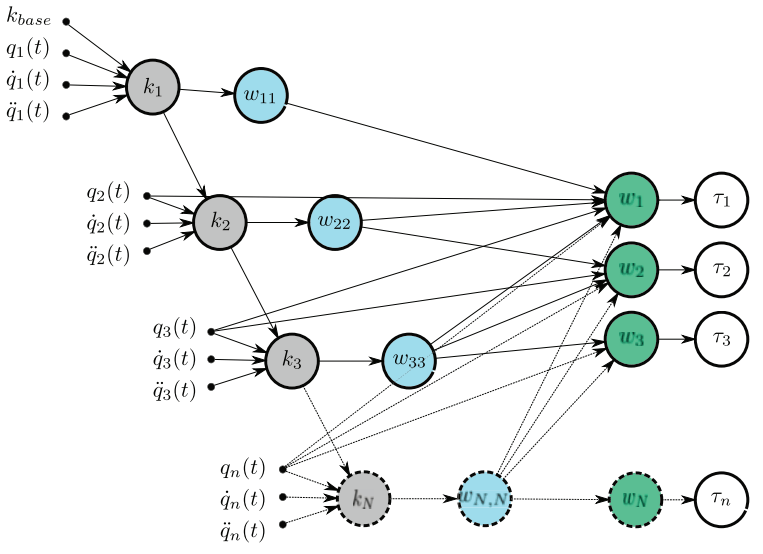
\includegraphics[width=0.495\textwidth]{slike/FOP2.png}}
    \caption[First-order principles network (FOPnet)]{First-order principles network (FOPnet) \cite{Ledezma2017}}
    \label{fig:FOP}
\end{figure}

The inverse dynamics of a robot is vital since models that are \emph{learned} can be used in place of analytical models that are usually required by the force observers, as emphasised previously in this section. 

An approach to learning the inverse dynamics of a robotic manipulator using Long-Short Term Memory (LSTM) networks at time $O(n)$ is presented in \cite{Rueckert2017}. This approach required an extensive data set of 100,000 samples, and using the proposed LSTM network, the prediction error decreases exponentially with the number of data samples used, and even for relatively small datasets, it shows better results than other modern approaches based on Gaussian processes. 

In \cite{Gupta2019} a novel framework for learning accurate dynamics of mechanical systems is proposed. The approach uses a ``grey-box'' model of a system in which the previous knowledge is incorporated where it is available, and otherwise, the estimators (i.e., neural networks) are trained. The ``grey-box'' model was used to address the variance vs bias issue, since the white-box model (i.e., parametrised, analytical model) introduces high bias and the black-box model (i.e., neural network) introduces high variance, as is shown in Figure \ref{fig:StructuredLearning}. The approach was applied on a simulated double pendulum. However, it should be easily extendable to the field of robotics, according to the authors. However, the limitation of the method is that it is more computationally expensive than pure black- or white-box models.

\begin{figure}
    \centering
    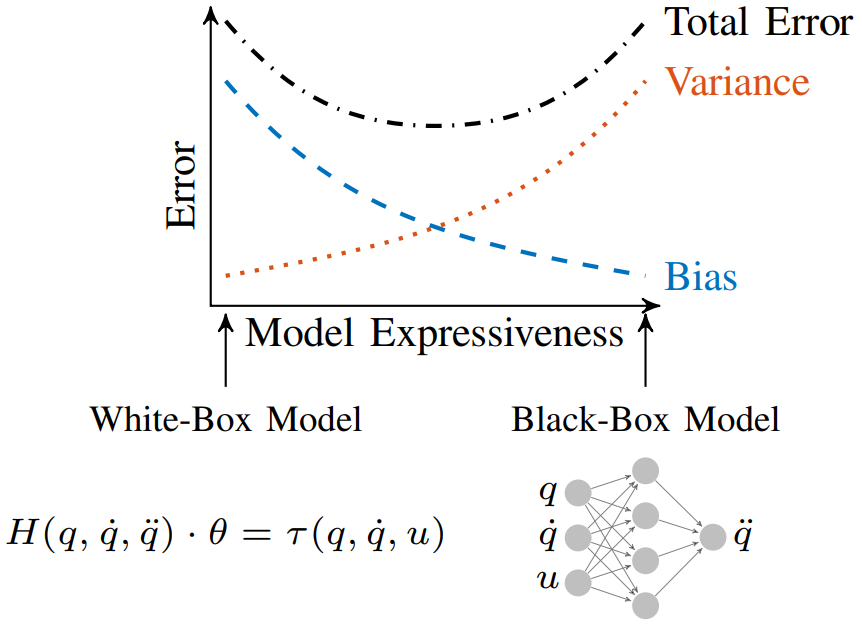
\includegraphics[width=0.5\textwidth]{slike/gupta2019.png}
    \caption[The bias-variance tradeoff]{The bias-variance tradeoff \cite{Gupta2019}}
    \label{fig:StructuredLearning}
\end{figure}

\newpage
\chapter{MATERIALS AND METHODS}
\label{chap:Materials}

The research in this dissertation deals with mobile robotic manipulators. As outlined in the literature review, the mobile manipulator can be controlled either as one coupled system or as two separate systems: a mobile base and a robotic manipulator, the latter being a case in this dissertation. Thus, the research can be broadly divided into two parts, one tackling the navigation of mobile base and the other deals with the estimation of forces acting on the manipulator end-effector, since those forces are the key to successful completion of tasks in which the robot interacts with a human, other robot or anything in its environment. 

First, a neural network-based obstacle avoidance method was developed, as described in Section \ref{sec:MMAvoidance} \cite{Kruzic2020,Kruzic2018}, which is then used in the fusion scheme called \emph{mediation}, described in Section \ref{sec:MMMediation} \cite{Music2019}. Finally, approaches to manipulator end-effector force estimation and joint torque estimation based on deep neural networks are presented in Section \ref{sec:MMForceEstimation} \cite{Kruzic2020a,Kruzic2021}. In each section, a problem is formulated, and a method to solve the problem is given. The appropriate experiments were conducted to assess the viability and performance of the presented solutions to the problems in question.

As neural networks were heavily used in the research, it is essential to emphasise methods and software used for their training. The training was conducted using Tensorflow 2 with Keras. All networks were initialised with a Glorot uniform initialiser \cite{Glorot2010}, and trained using Adam optimiser \cite{Kingma2014}, starting with a learning rate of 0.001. However, since the optimiser is adaptive, the learning rate changed during the training. The mean absolute error (MAE) and mean squared error (MSE) were used as loss functions in the training process, while ReLU and ELU functions were used for activating neurons. Finally, as a performance metric, the root-mean-squared error (RMSE) function was used. In all instances, the training lasted until there was no improvement in validation loss for five consecutive epochs. For hyperparameter optimisation, Hyperband algorithm\cite{Li2018} was used, implemented in Keras Tuner, a part of Tensorflow-Keras framework.


\section{Neural network-based obstacle avoidance for mobile robots}
\label{sec:MMAvoidance}

\subsection{Problem formulation}

The goal of this part of the research was to develop a procedure to train and test an efficient neural network architecture for mobile robot obstacle avoidance while keeping human intervention as minimal as possible (i.e., self-supervised nature) \cite{Kruzic2020a}, and to deploy it onto the real-world robot. The approach should provide numerous positive and negative examples (crashes) to the learning algorithm but should safely do that for the robot and its environment.  It should also enable the collection of large amounts of data with minimal effort and cost. To that end, it was decided to use 2D LiDAR (laser distance sensor) instead of a camera. Although cameras can provide much richer data than LiDAR, LiDAR is sufficient for obstacle avoidance. However, it should be kept in mind that LiDAR sensing can fail in some instances (e.g., in the presence of glass surfaces or if the distance is below or above the sensing threshold). Furthermore, the LiDAR output is less complex than the video stream, making the neural network architecture simpler and shorter training time. This less complex nature of input data has an attractive side effect that real-world measurements are more similar to simulation-based ones than in the case of a video stream. Finally, mass-produced and low-cost LiDARs are on the horizon, making them a logical choice for one of the mobile robot's primary sensors for the future.

There are two fundamental reasons why simulation was chosen for conducting this part of the research. The first one is that crashing a real robot into obstacles may damage both the robot and the obstacle. The other is that the usage of simulation makes possible the collection of large amounts of data with different crashing scenarios with minimal effort and negligible cost, yet achieving a high degree of similarity between data obtained in simulation compared to real-world data by using LiDAR sensor. An additional reason for using a simulation environment is that the whole approach (including neural networks) can be fine-tuned in simulation and deployed only when an acceptable level of performance is achieved (as was done in the research).

Differences between the simulated camera and LiDAR compared to the real-world camera and LiDAR data are illustrated in Figure \ref{fig:Fig01}. From the figure, it can be seen that differences exist between the simulation and real-world cases both for LiDAR and camera. However, due to different lighting conditions (which are difficult to reproduce in simulation) and the existence of textures and shadows, the image-based comparison produces more significant discrepancies than the LiDAR-based one. Please note that the same distance from the robot to obstacles was used in both scenarios. It should be noted that recently approach which uses simple graphics (i.e., not photorealistic) but with a substantial number of variations in light and texture (for better generalisation) have been investigated, and good results reported in the domain of robotic grasping \cite{Bousmalis2018}.

\begin{figure}
    \centering
    \subfloat[Camera image from simulation environment]{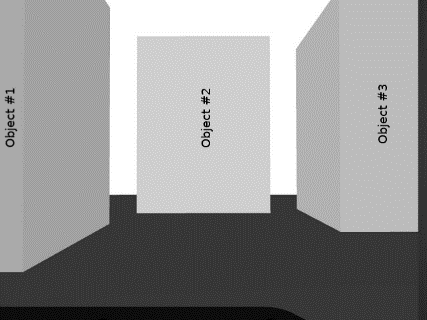
\includegraphics[width=0.45\textwidth]{slike/Fig03_01a.png}}
    \hfill
    \subfloat[Camera image from real robot]{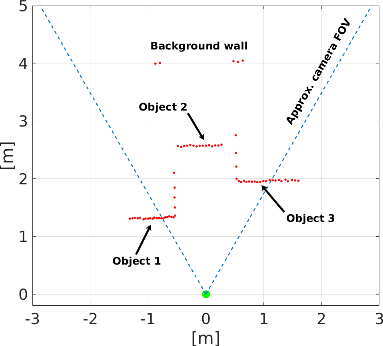
\includegraphics[width=0.45\textwidth]{slike/Fig03_01b.png}}
    \vfill
    \subfloat[LiDAR data from simulation environment]{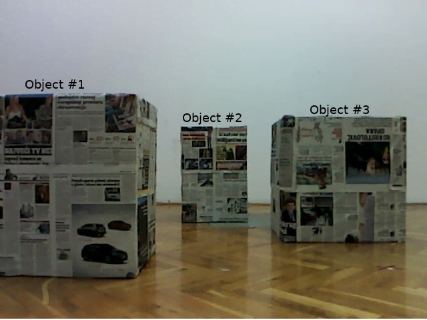
\includegraphics[width=0.45\textwidth]{slike/Fig03_01c.png}}
    \hfil
    \subfloat[LiDAR data from real robot]{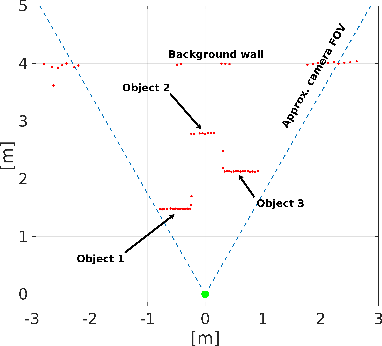
\includegraphics[width=0.45\textwidth]{slike/Fig03_01d.png}}
    \caption{Differences between camera images and laser scans in simulation and on the real robot of the approximately same scene.}
    \label{fig:Fig01}
\end{figure}

Please note that, although simulation-based neural network training approaches do exist in the literature (as is already presented in Chapter \ref{chap:Literature}), they usually employ cameras (which provide RGB images), use complex convolutional neural networks for obstacle avoidance, do not collect both positive and negative examples, and do not perform the neural network training process automatically. The focus of this part of the research was thus to develop the approach that would enable collecting the appropriate amount of data needed for training neural networks for obstacle avoidance in a self-supervised manner in simulation. Furthermore, it should also be confirmed that simulation-driven LiDAR data can be effectively used for training neural networks. Finally, it should also be demonstrated that seamless transfer to real-world applications is possible and that such neural networks perform well in the real world compared to some common obstacle avoidance algorithms.

\subsection{Data collection and labelling}

Training data for obstacle avoidance was generated and collected in Gazebo simulation environment \cite{Koenig2004} as follows. First, a simulation was automatically initialised, and various obstacles were randomly scattered within it, as is shown in Figure \ref{fig:Fig02}. The dimensions of the simulated environment were always kept the same (12.5 m $\times$ 12.5 m) but can be freely chosen/changed by the user. Then, the robot was spawned in its centre with random orientation and was given a constant linear velocity of 0.4 m/s. While the robot was in motion, LiDAR data were collected. The recording was carried out until the robot crashed into the obstacle or the perimeter wall (detected by the simulation engine).

\begin{figure}
    \centering
    \subfloat[Gazebo world and various obstacle shapes. Please note that obstacles had footprints of 0.5 m $\times$ 0.5 m for cubes, 4 m $\times$ 0.8 m for cuboids and 0.5 m $\times$ 0.5 m for cylinders.]{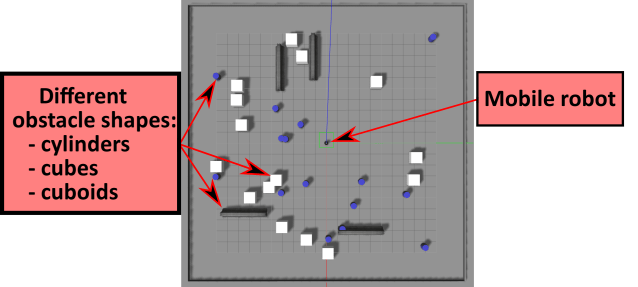
\includegraphics[width=0.9\textwidth]{slike/Fig03_02a.png}}
    \vfill
    \subfloat[Examples of different randomly generated Gazebo Worlds]{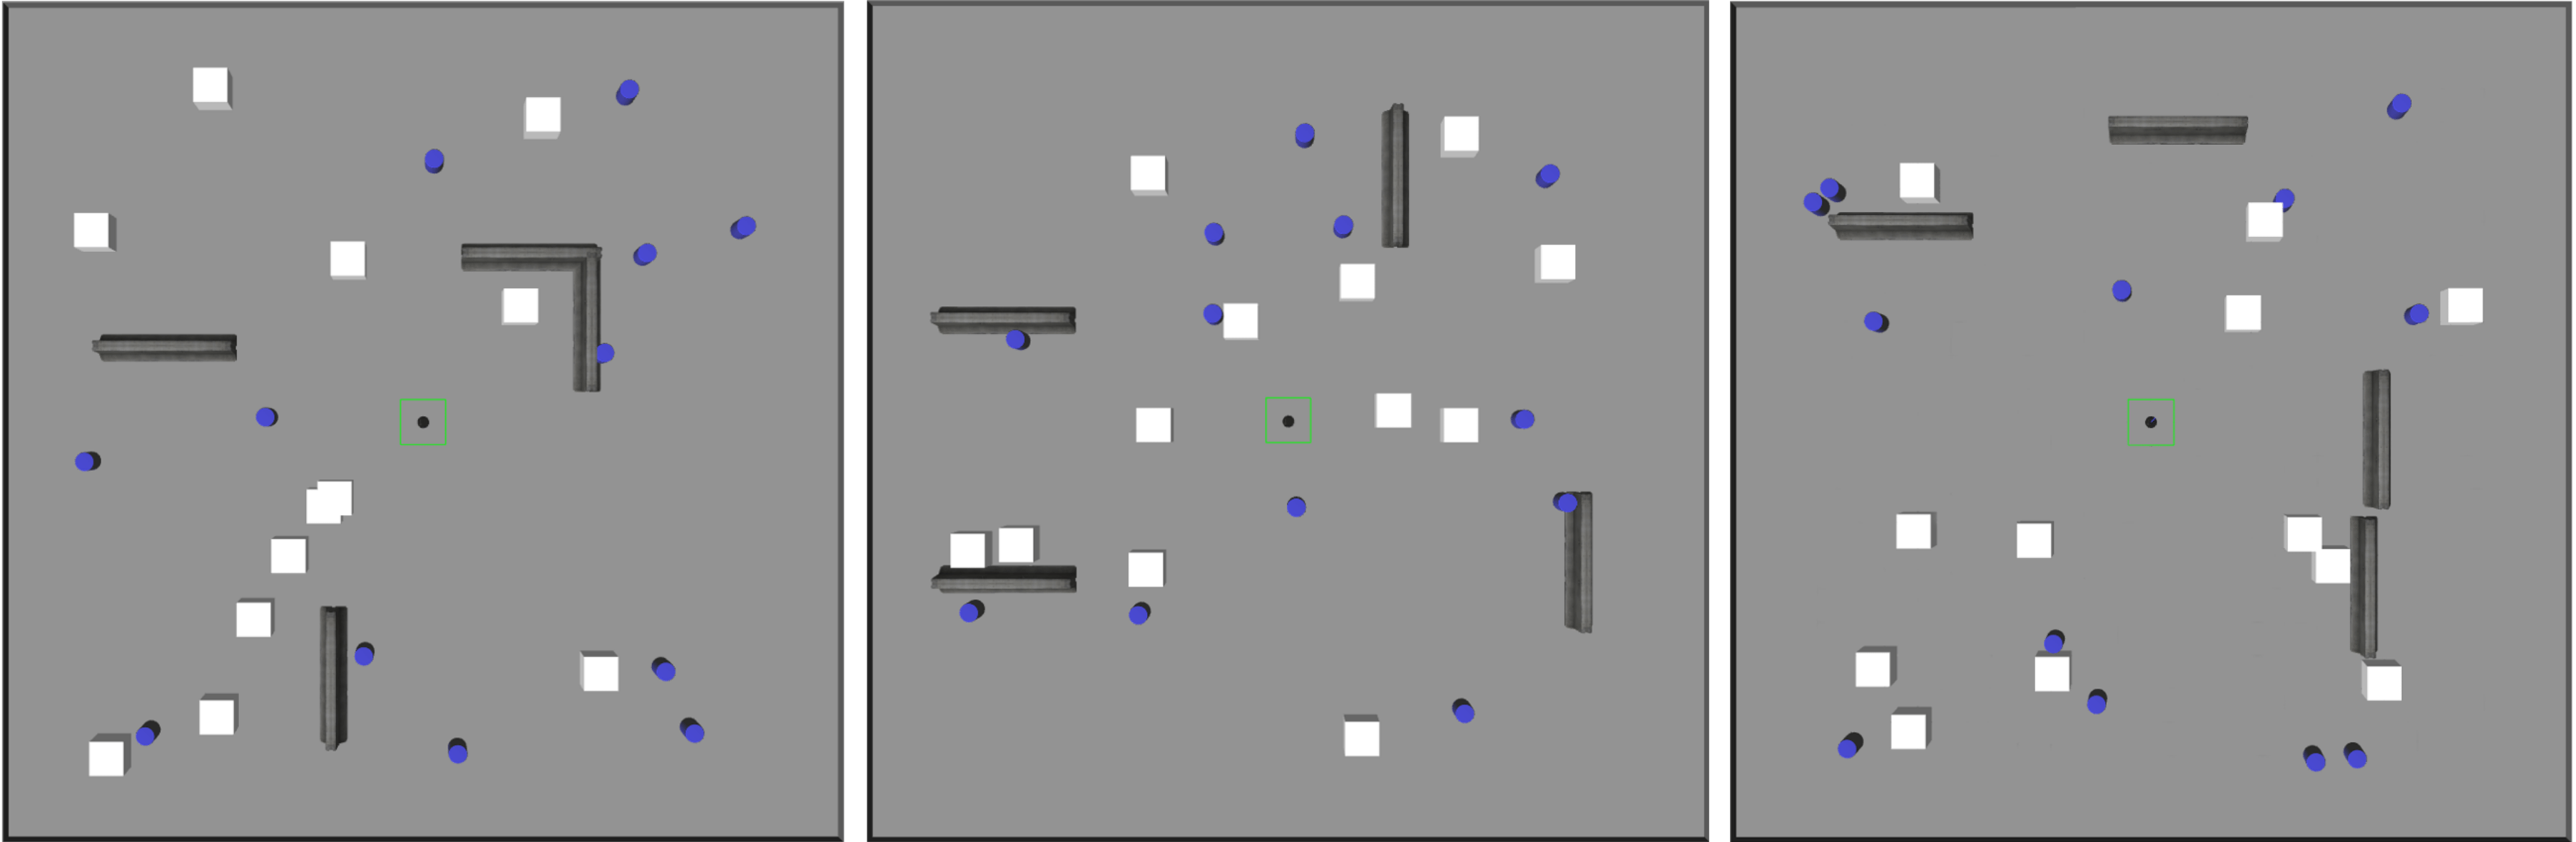
\includegraphics[width=0.9\columnwidth]{slike/Fig03_02b.png}}
    \caption{Gazebo simulation environment}
    \label{fig:Fig02}
\end{figure}

The laser range finder scans were timestamped, and the timestamp of the moment when the robot hits the obstacle was also recorded. The preceding procedure is repeated many times (specified by the user) to obtain enough data for the neural networks to generalise appropriately. In the experiments, a total of 3,754 crash events were obtained (in 19 simulation worlds with different obstacle setups), which took about two workdays of real-time self-supervised execution (with no human intervention) on a computer with an Intel Core i3 6100 processor and 4 GB of RAM. The described data collection procedure resulted in 396,377 training samples both positive (no crash) and negative (a crash and a period shortly before the crash).

Before the training of the neural networks, the obtained data were preprocessed. First, failed LiDAR measurements were replaced with maximal possible range values. Failed measurements occurred when the obstacle was closer than the declared minimum sensor range (0.15 m) or farther away than the maximum (6 m). Obtained scan data was then divided into three overlapping groups, so each of the three networks was trained on a different dataset. The network for the forward motion used scans of 45$^{\circ}$ to both left and right of forward direction (90$^{\circ}$ in total), while the network for left and right motion used scans of 90$^{\circ}$ to the left and the right of the forward direction. This is graphically depicted in Figure \ref{fig:Fig03} (from the robot's viewpoint).

The last two seconds of the robot motion before the collision were treated as negative examples (this duration was always guaranteed since there were no obstacles in an appropriate diameter around the robot's initial position), but only for the network(s) representing the side of the robot on which the bumper was activated during the collision. In contrast, the other sides' network labels remained positive. If a particular measurement lasted longer than 4 s, the first 2 s were treated as positive examples while the remaining (middle) part of the data samples (excluding the last two seconds) was discarded and not used for training. Otherwise, all remaining data samples were treated as positive examples.

\begin{figure}
    \centering
    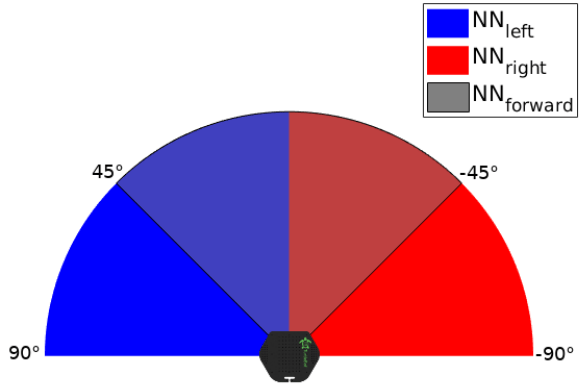
\includegraphics[width=0.75\textwidth]{slike/Fig03_03.png}
    \caption{LiDAR scans divided into three overlapping groups (left, forward, right)}
    \label{fig:Fig03}
\end{figure}

After initial labelling, all the labels are further examined, and those that are positive are converted to negative if there were some laser scan points closer than the predefined threshold. The relabelling procedure was conducted to prevent motion near the obstacles that did not result in a crash. An example of such a situation would be a robot moving parallel to the wall. The decision about if a label needed to be converted to negative was made based on two parameters: the number of laser scan points and the threshold. Both parameters varied during the study (using predefined values of 3, 5, and 7 for the points and 0.4 m, 0.6 m, 0.8 m and 1 m for thresholds). The procedure of how a label is classified using these numbers of points and thresholds is given in Figure \ref{fig:Threshold}. The label is negative if there are 3, 5 or 7 LiDAR points under the appropriate dashed line, depending on the chosen threshold value. 

\begin{figure}
    \centering
    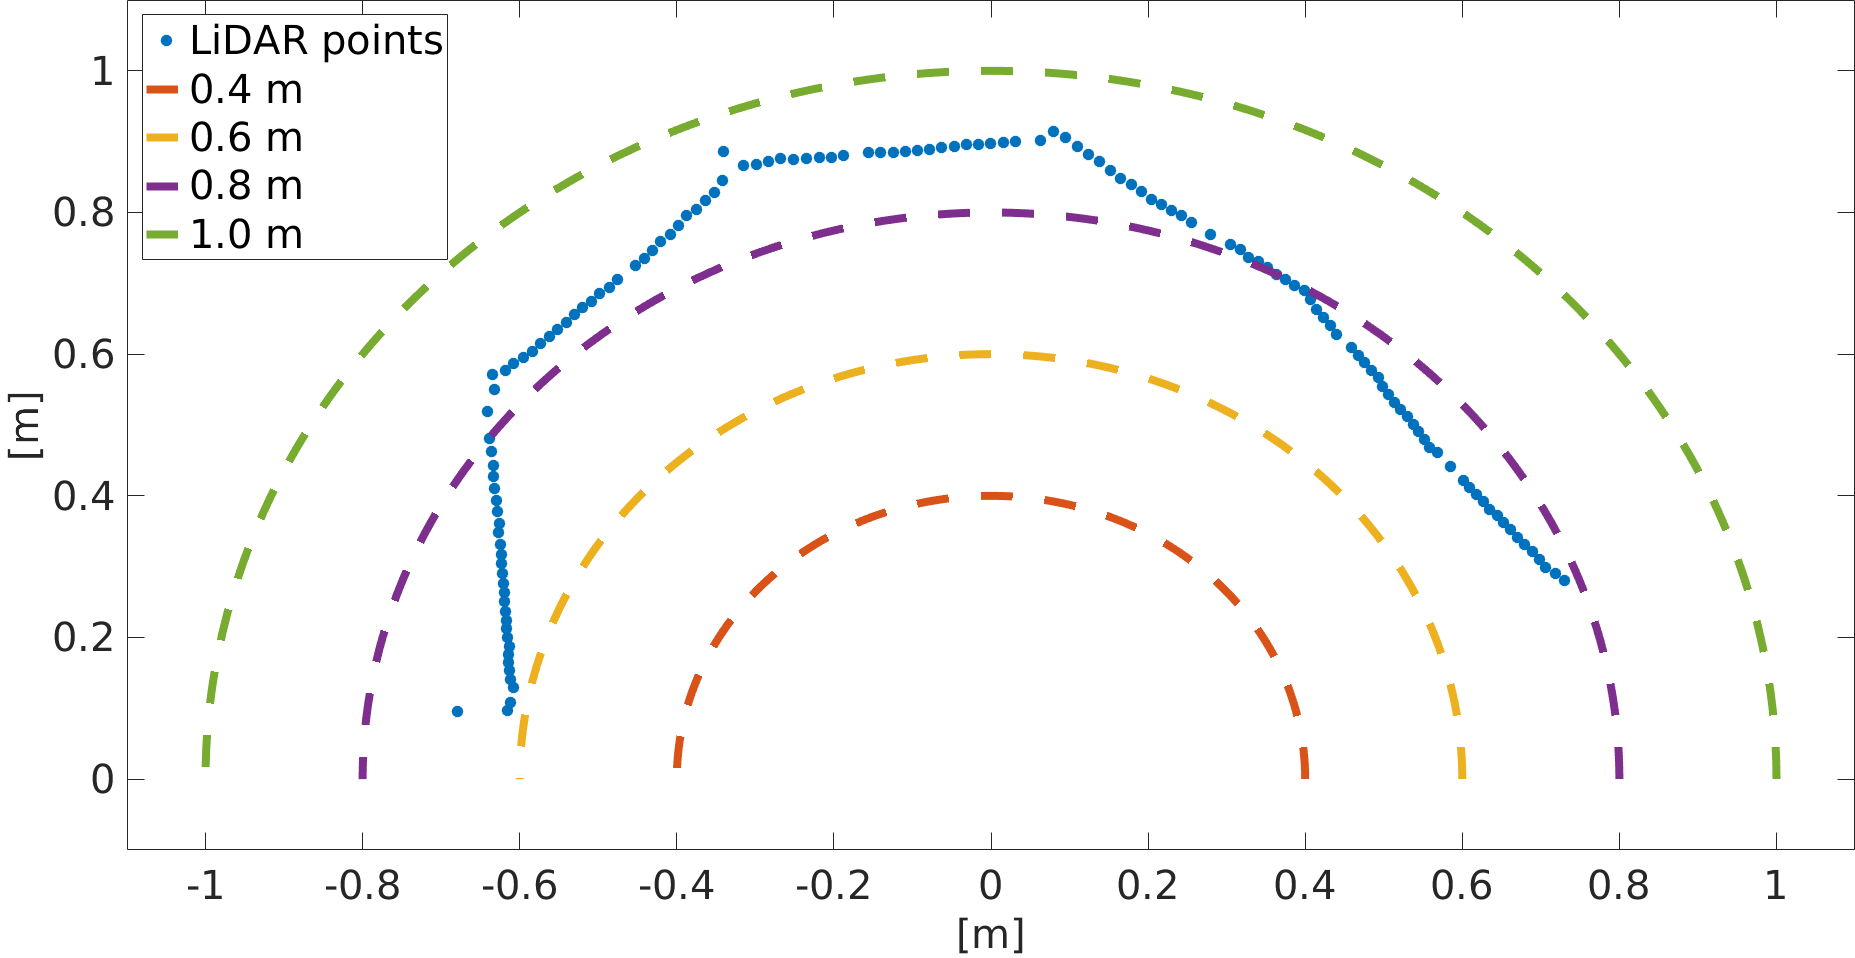
\includegraphics[width=0.9\textwidth]{slike/Fig03_04.png}
    \caption{The classification of LiDAR scan points in the presence of a complex obstacle}
    \label{fig:Threshold}
\end{figure}

In such a way, 12 datasets were created to identify which pair of parameters (number of points, threshold) were optimal for the task. Then, neural networks were trained for each pair of values for the number of points and a threshold to identify which pair of these values performs best for the task \cite{Kruzic2018}. The intention was to keep neural networks trained with data from the dataset with parameters that were proved optimal and use them for further experimenting.

The whole labelling and neural networks training procedure is given as Algorithm \ref{Alg:Preprocess}.

\begin{algorithm}
\caption{Data preprocessing and neural networks training procedure}
\label{Alg:Preprocess}
\begin{algorithmic}
	\renewcommand{\algorithmicrequire}{\textbf{Input:}}
    \renewcommand{\algorithmicensure}{\textbf{Output:}}
    \REQUIRE LiDAR scan with 1$^{\circ}$ resolution $S=\{S_1,S_2,...S_{360}\}$
    \STATE Replace failed measurements in $S$ with max LiDAR range
    \STATE Forward scans: $S_F \gets S_{1:45} \cup S_{316:360}$
    \STATE Left scans: $S_L \gets S_{1:90}$
    \STATE Right scans: $S_R \gets S_{271:360}$
    \STATE Number of points: $P \gets \{3,5,7\}$
    \STATE Thresholds: $T \gets \{0.4, 0.6, 0.8, 1.0\}$
    \FOR {$p$ in $P$}
      \FOR {$t$ in $T$}
          \STATE Label $S_F$, $S_L$, $S_R$ using $p$ and $t$
          \STATE Train $\mathrm{NN}_F^{(p,t)}$, $\mathrm{NN}_L^{(p,t)}$, $\mathrm{NN}_R^{(p,t)}$
      \ENDFOR
    \ENDFOR
    %\ENSURE $\mathrm{NN_F}$, $\mathrm{NN_L}$, $\mathrm{NN_R}$
    \ENSURE $\{\mathrm{NN}_F^{(p,t)}$, $\mathrm{NN}_L^{(p,t)}$, $\mathrm{NN}_R^{(p,t)} \mid p \in P \land~t \in T\}$
\end{algorithmic}
\end{algorithm}


\subsection{Neural networks training}

The neural network-based controller was designed to have three independent neural networks: left, forward, and right. Several network architectures were considered and trained using different hidden layers numbers (1 to 4) and different numbers of neurons per layer (20, 40, 60, 80). Thus, it amounted to 16 different network architectures per direction (left, right and forward), giving 48 architectures whose performance was analysed. Each network was trained as a multilayer perceptron, with SGD as the optimiser and MSE as the loss function (and performance metric). The performance of all trained networks was analysed on the validation set (the analysis is given in \cref{Sec:ResLabelling}). Based on the analysis, the best architecture for the task is identified.

Once the best architecture was identified, the neural network was trained with samples from randomly selected 75\%, 50\% and 25\% of data samples (297,283, 198,189 and 99,095 training samples, respectively) in order to approximately estimate the number of training samples needed for proper generalisation of neural networks. 

Based on the neural network outputs, linear and angular velocity commands are computed using the policy in Algorithm \ref{Alg:Policy} as follows. Each neural network output was between 0 and 1, which is the probability that the space in the appropriate direction is obstacle-free. Alternatively, one may think of this as the output of 1 meaning \emph{``go in this direction''} and 0 meaning \emph{``do not go in this direction''}. Network outputs are post-processed to obtain linear ($v$) and angular ($\omega$) velocities for robot motion. If the forward direction probability ($P(F)$) was above a predefined threshold of 0.5 (which was determined experimentally), then the direction was computed as a proportion to a difference between probabilities of left and right directions ($P(L)$ and $P(R)$, respectively) being obstacle-free. If the forward direction probability were below the threshold, the robot would slow down to a low positive velocity and not stop to avoid local minima (also experimentally determined and explained in Section \ref{Sec:ResLabelling}) and rotate either to the left or right depending on which side is obstacle-free. Once forward-facing neural network probability increased above the threshold, it would speed up and continue as before. Thus, it can be concluded that linear velocity had two predefined levels, while the angular velocity could attain any value between -2 rad/s and 2 rad/s, and the value is computed using Equation \ref{eq:AngularVelocity}.

\begin{algorithm}
\caption{Obstacle avoidance policy used in testing}
\label{Alg:Policy}
\begin{algorithmic}
	\renewcommand{\algorithmicrequire}{\textbf{Input:}}
    \renewcommand{\algorithmicensure}{\textbf{Output:}}
    \REQUIRE Scans $S_F$, $S_L$, $S_R$, neural networks $NN_F$, $NN_L$, $NN_R$
    \STATE Forward probability: $P(F) = NN_F(S_F) \in [0,1]$
    \STATE Left probability: $P(L) = NN_L(S_L) \in [0,1]$
    \STATE Right probability: $P(R) = NN_R(S_R) \in [0,1]$
    \IF {$P(F)>0.6$}
    	\STATE $v=0.4$ m/s
        \STATE $\omega\propto P(L)-P(R)$
    \ELSE
    	\STATE $v=0.08$ m/s
        \IF {$P(L)>P(R)$}
        	\STATE $\omega\propto P(L)$
        \ELSE
        	\STATE $\omega\propto -P(R)$
        \ENDIF
    \ENDIF
    \ENSURE $(v,\omega)$
\end{algorithmic}
\end{algorithm}

\begin{gather}
    \label{eq:AngularVelocity}
    \omega = \begin{cases}
        \hphantom{-}2 \cdot P(L) & P(L) \geq P(R)\\
        -2 \cdot  P(R) & P(L) < P(R)
    \end{cases}\\
    P(L), P(R) \in [0,1] \nonumber
\end{gather}

\subsection{Experimental setup}

Several experiments were performed to assess the performance of the proposed approach to neural network-based obstacle avoidance. The first experiment was conducted to identify optimal parameters for data labelling. The obtained results from that experiment are then used in other experiments, both in simulation and in the real world, to show that neural networks trained on simulation data can perform well without any retraining.

\subsubsection{Parameters identification experiment}
\label{Sec:MMLabelling}

This experiment was conducted to assess the performance of neural networks trained on simulation data and aimed to identify optimal parameters for the number of LiDAR points and threshold. The environment for testing the approach was a relatively narrow (2.16 m) corridor augmented with additional obstacles, as shown in Figure \ref{Fig:Hodnik}.

\begin{figure}
\centering
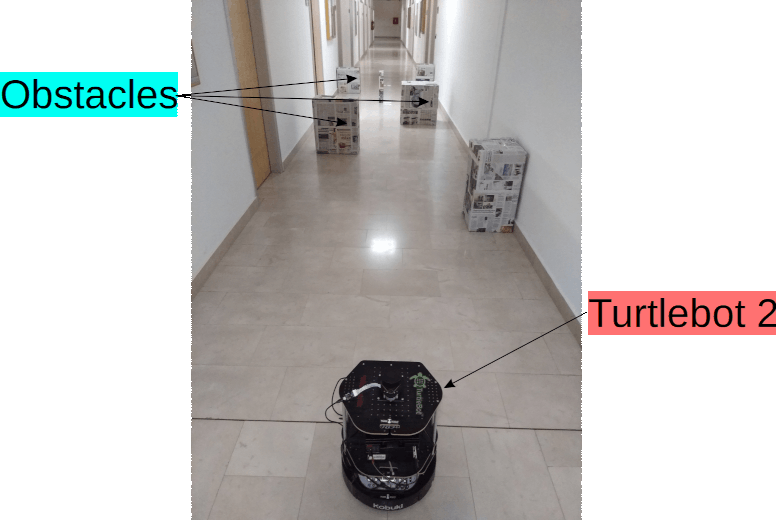
\includegraphics[width=0.8\textwidth]{slike/Fig03_05.png}
\caption{A corridor augmented with additional obstacles}
\label{Fig:Hodnik}
\end{figure}

Each of 12 datasets was used for testing with five trials per dataset, resulting in 60 trials. The robot was left to roam the course freely. There was no allocated time frame for task completion. However, there were four events in the case of which a trial terminated: completion of the course (i.e. going beyond the last obstacles on the course, see Figure \ref{Fig:LabellingTraj}), crash into obstacle or walls, stuck in a loop (i.e. repeating the same motions over and over) or stuck at local minimum (i.e. when moving forward is not possible, and when robot executes in-place rotation left and right interchangeably).

The results of this experiment were given and analysed in Section \ref{Sec:ResLabelling} and, once when best parameters were identified, neural networks trained with those parameter values are used in all of the following experiments regarding obstacle avoidance.

\subsubsection{Simulation experiments}

The first experiment was conducted in simulation in four random environments that were generated the same way as were those used for collecting training data and shown in Figure \ref{fig:Fig02}. There were five test runs in each of the environments (20 test runs in total). Each run began with the robot in the centre with a random orientation. It lasted until the robot crashed into the obstacle, or a maximum time limit of 10 minutes was reached.

The second simulation experiment was straightforward and was conducted in a small 5 m x 5 m environment with a single moving obstacle, as depicted in Figure \ref{fig:Fig07}. The robot was left for 10 minutes to roam around the environment. The experiment was run four times, each time with a different (but constant) obstacle velocity (0.1 m/s, 0.2 m/s, 0.4 m/s and 0.8 m/s; please note that in the Figure \ref{fig:Fig07}, the obstacle moved left and right in the directions indicated by the arrows). 

\begin{figure}
    \centering
    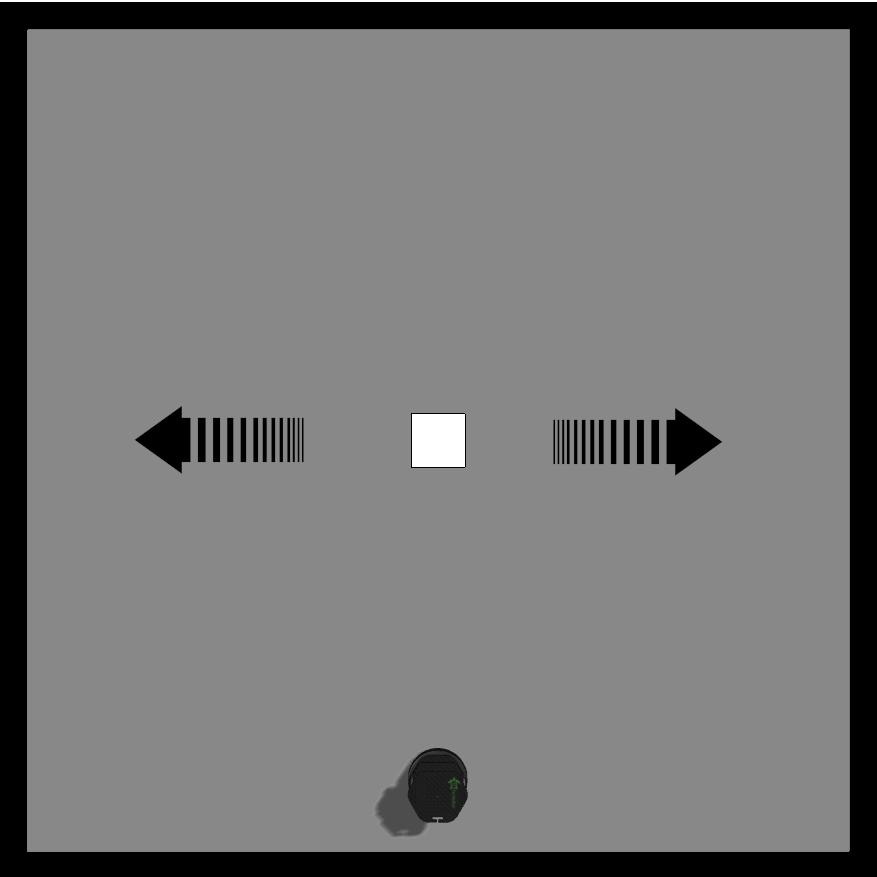
\includegraphics[width=0.5\textwidth]{slike/Fig03_06.png}
    \caption{Simulation environment for testing robot behaviour in the presence of moving obstacle. Arrows indicate motion directions of the moving obstacle.}
    \label{fig:Fig07}
\end{figure}

\subsubsection{Real-world experiments}

The experiments in the real world were conducted using a real robot, a heavily modified Turtlebot 2 mobile robot (shown in Figure \ref{fig:Fig08}), with a LiDAR sensor mounted on-board. The 2D LiDAR used was Rplidar-A1M8, which has a resolution of 1 degree (i.e., gives 360 points per measurement cycle) and run with a 7 Hz rotation frequency and a distance range of 6 m. 

\begin{figure}
    \centering
    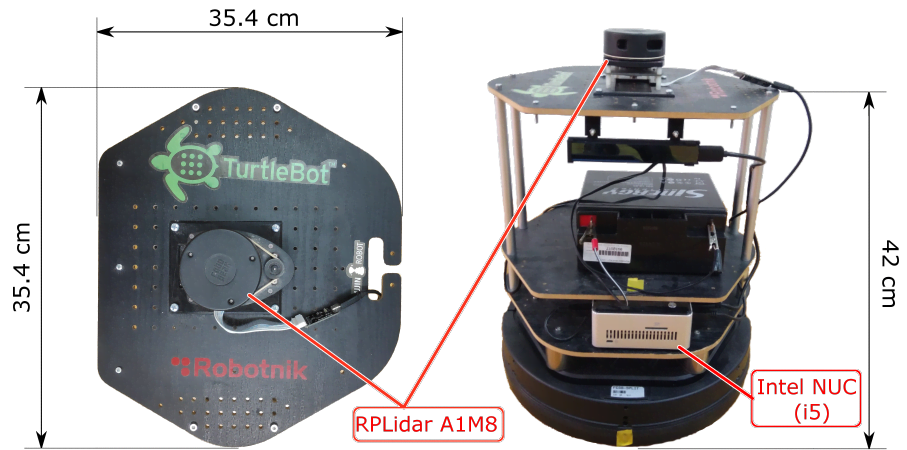
\includegraphics[width=0.8\textwidth]{slike/Fig03_07.png}
    \caption{Turtlebot 2 mobile robot, used in real-world experiments}
    \label{fig:Fig08}
\end{figure}

In the first real-world experiment, a U-shaped obstacle was used to test how well the neural network recovers from such a complex obstacle and a challenging situation. 

\begin{figure}
    \centering
    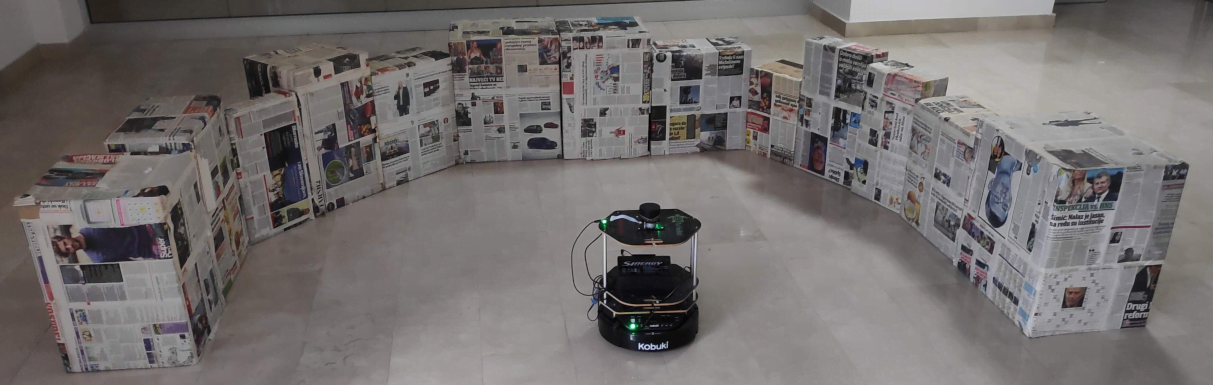
\includegraphics[width=\textwidth]{slike/Fig03_08.png}
    \caption{The experimental setup for the U-shaped test case}
    \label{fig:UshapeExp}
\end{figure}

In contrast, in the second one, a narrow (only 2.16 m wide) corridor was augmented with additional obstacles making it more demanding for the obstacle avoidance algorithm. The experimental setup for this experiment is similar to the parameters identification experiment. However, the dataset used for the training neural networks was preprocessed with the values identified in the mentioned experiment, and there were fewer obstacles (but the same corridor was used). In this test case (\cref{fig:CorridorExp}), obstacles were placed in such a manner that it could be, with a high degree of certainty, assumed that the obstacle avoidance will fail (since free gaps at the last obstacle - rightmost one in Figure \ref{fig:Fig10c} - are well below the clearances used in training).

\begin{figure}
    \centering
    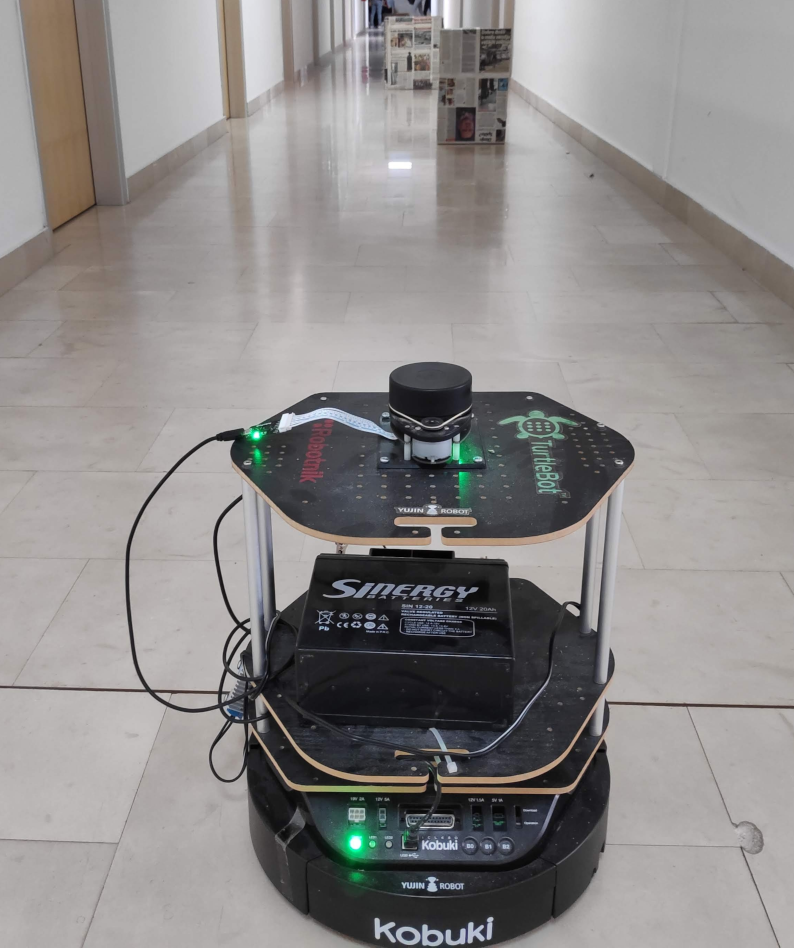
\includegraphics[width=0.4\textwidth]{slike/Fig03_09.png}
    \caption{The experimental setup for the narrow corridor test case}
    \label{fig:CorridorExp}
\end{figure}

Afterwards, the proposed approach was compared to a baseline obstacle avoidance algorithm shipped with ROS (Robot Operating System) \cite{Quigley2009} navigation stack - Dynamic Window Approach (DWA) \cite{Fox1997}. The measurement setup was pretty simple, with the robot always starting from the same point in space and having to go to the point behind a simple rectangle-shaped obstacle that was not in the original map.

In the final real-world experiment, the robot was placed inside a complex, self-contained obstacle course (similar to the simulated environment) which is shown in Figure \ref{fig:Fig12}, and in which it freely ran for 20 minutes. The course also had dynamic obstacles (moving mobile robots Turtlebot 3 Burger and Waffle) with predefined trajectories. The number of collisions, the time between collisions as well as the distance between collisions were recorded. 

\begin{figure}
    \centering
    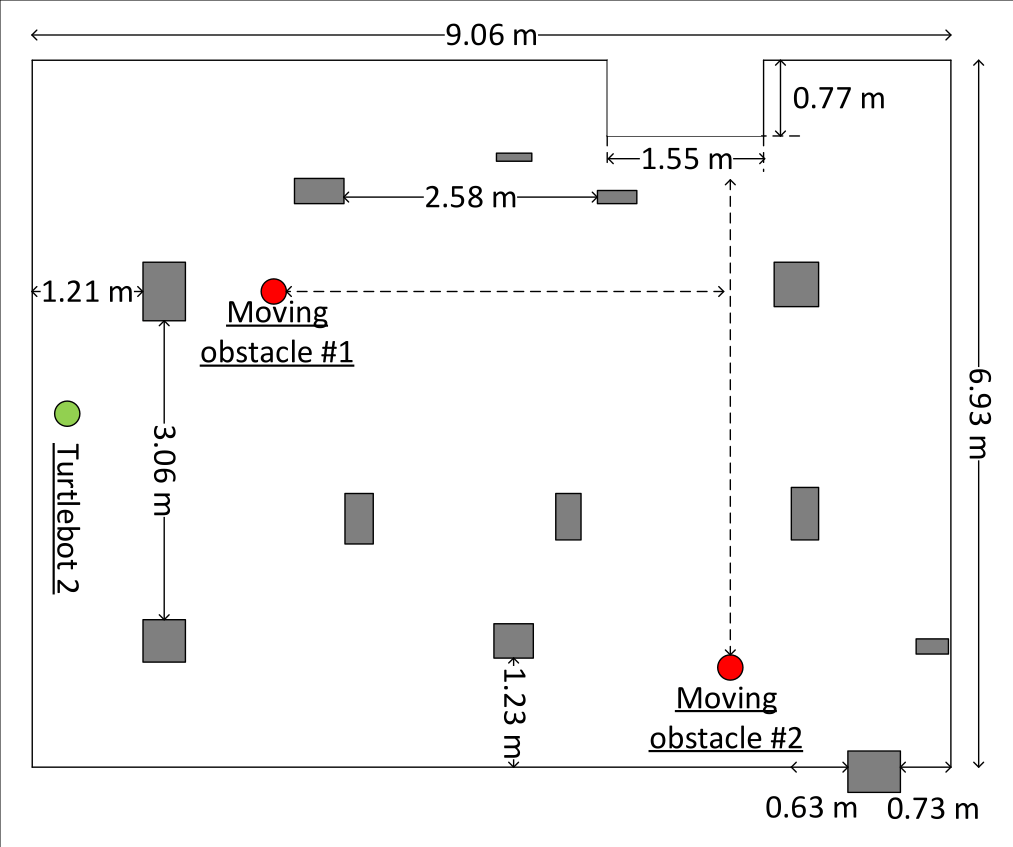
\includegraphics[width=0.775\textwidth]{slike/Fig03_10.png}
    \caption{Floor plan of the real-world testing environment with static and dynamic obstacles}
    \label{fig:Fig12}
\end{figure}

\section{Mediated navigation in mobile robotics}
\label{sec:MMMediation}

\subsection{Problem formulation}
\label{sec:MMMediationFormulation}

From the literature review, it can be concluded that deploying state-of-the-art autonomous capabilities to a mobile robot usually entails developing complex neural network-based architectures and training them in an end-to-end fashion on large datasets (either in a simulation or in a real-world environment). Furthermore, if different behaviour is required, a new network needs to be developed or an existing one retrained (and new training data generated or recorded). 

It is desirable to develop an approach to mobile robot navigation that could use existing control algorithms and combine them with artificial intelligence. In the field of control theory, there exist approaches by which complex robot behaviour is achieved by \emph{mediation} between two desired behaviours \cite{Vincenti2009}. Therefore, complex behaviours, such as navigation, can be divided into simpler ones (tasks). Thus, for each simple behaviour, another controller can be introduced. With this approach, it is possible to achieve that performing slightly different robot tasks does not entail changing the whole approach to the problem. Thus, it is enough to change one of the controllers in charge of the behaviour, saving time and achieving complex mobile robot behaviour patterns. 

Implementing a mediator that would enable the fusion of control signals from several sources (including, but not limited to, neural networks) is proposed to avoid training new networks when the new behaviour is required. One possible function on which adaptive control in mobile robot navigation tasks could be based is collision probability \cite{Lunenburg2017} since obstacle avoidance usually has the highest priority in the navigation stack hierarchy. The mediation can be implemented in several forms, and one of them is based on fuzzy set theory \cite{Chen2017}. It is worth noting that several \emph{mediation engines} can be used in the process, as well as several decision functions based on which the mediator infers the final decision and thus adapts the robot behaviour \cite{Vincenti2009}.

Overview of the proposed adaptive fuzzy control scheme can be seen in Figure \ref{Fig:Blok} which shows that the approach uses two controllers (neural networks or any other type of controller) whose inputs are combined within fuzzy set theory based on the collision probability as the decision variable. The newly developed collision probability parameter is explained in more detail later on.

\begin{figure}
\centering
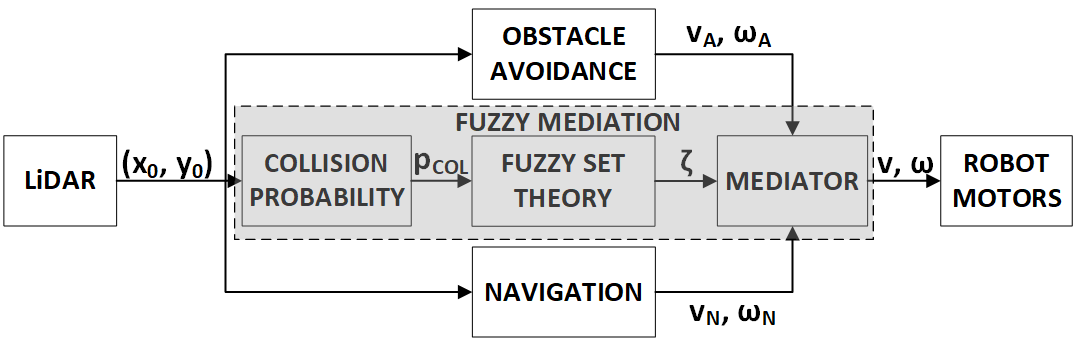
\includegraphics[width=0.95\columnwidth]{slike/Fig03_11.png}
\caption{The general control architecture of the proposed approach.} 
\label{Fig:Blok}
\end{figure}

In the proposed approach, one controller was used for reaching the goal position without regard to obstacles (navigation controller), while the other controller was used solely for obstacle avoidance without regard to the goal position. Furthermore, both controllers (in the case of neural networks) were trained using data obtained in the simulation, making the proposed approach safe and straightforward. 

The neural network-based obstacle avoidance controller that was used in this part of the research consisted of three neural networks (for left, right and forward) and is described in detail in Section \ref{sec:MMAvoidance} with Algorithm \ref{Alg:Policy} used to generate velocity commands as outputs of the controller. The velocity part of the command is always at one of two predefined levels (0.4 m/s and 0.08 m/s), and the angular velocity is given as

\begin{gather}
    \label{eq:AngularVelocity2}
    \omega_A = \begin{cases}
        \hphantom{-}2 \cdot P(L) & P(L) \geq P(R)\\
        -2 \cdot  P(R) & P(L) < P(R)
    \end{cases}\\
    P(L), P(R) \in [0,1] \nonumber
\end{gather}

Please note that the Equation \ref{eq:AngularVelocity2} is just rewritten version of the Equation \ref{eq:AngularVelocity} to accommodate the notation used in Figure \ref{Fig:Blok}.

In the case of the development of a neural network for navigation, the following procedure was taken. First, a single user was asked to drive a Turtlebot 2 mobile robot in the Gazebo simulation from a random starting point to a random goal within a 25 m $\times$ 25 m environment without any obstacles. The driver was instructed to give equal importance to the accuracy and the speed of driving. During the driving, the robot position was recorded, thus making it possible to calculate the distance from the goal. This procedure was repeated 700 times, giving a total of 380,541 training examples. After that, the recorded data was used to train a simple neural network (for regression) with four layers of 30 neurons each. This architecture was (as was the case for neural network-based obstacle avoidance) determined experimentally as the one with \emph{good enough} performance, and thus better architectures might exist. As an input, the network was given the error in position (i.e., distance to the goal) and orientation (i.e., the difference between the current and the final orientation). In addition, the network was given both the linear and angular velocities recorded during the trials as the network targets. Also, these were used as its output during testing. After the training, the approach was tested successfully in environments without obstacles, both in simulation and real life. 

Additionally, in cases when a simple Proportional (P)-type controller was used, its output was such that it kept the linear velocity ($v_N$) constant till the goal was reached. In contrast, angular velocity ($\omega_N$) changed depending on the difference between the current and desired position (both in the odometer frame of reference). In this manner, both the simple and more complex (neural network-based) cases of navigation controllers were taken into account.

The outputs from the neural network-based obstacle controller and from the navigation controller (being any of the types used in the research) were then fed to the fuzzy mediation block, where the consensus decision was made (based on $\zeta$ value) and adapted linear ($v$) and angular ($\omega$) velocities were generated. The fuzzy mediation is explained further in the following section.

\subsection{Collision probability and fuzzy mediation}

 The mediation block in Figure \ref{Fig:Blok} firstly computes the collision probability ($p_{\textrm{COL}}$) based on LiDAR measurements and simplified robot kinematic model. Collision probability was designed in such a way to be reliable and computationally efficient while providing the mediation algorithm with necessary information. Although similar variables do exist in the literature, they are not as simple and computationally effective \cite{Coenen2014} as the proposed one.

Collision probability was calculated in several simple steps as described hereon. First, an estimated trajectory of the robot for the subsequent 20 samples (about 2 seconds) was computed based on a simple kinematic model of motion. The interval of 20 samples was chosen through experimentation as the one that, taking into account planned robot velocity (0.2 m/s) and the distance at which the neural network-based obstacle avoidance reacts, provides a sufficient time horizon for reaction. During the development, different interval lengths were tested. Longer intervals produced trajectory estimates that were less likely to occur, resulting in the robot giving control to the obstacle avoidance controller when in reality it did not need to, while shorter intervals produced much more likely trajectory estimates but reduced significantly reaction time for the robot resulting in a jittery motion and number of obstacle crashes. Thus, it was concluded that for the selected mediator parameters (and distance for obstacle avoidance for which the neural network was trained), the interval length is primarily a function of the robot linear velocity (and other parameters to a lesser extent). This perceived dependency should, however, be revisited if in-place rotation is introduced. Thus, if different robot speed, sampling time, or allowed distance to the obstacles during neural networks training (1 m in our case) was used, the interval value should be adjusted accordingly. The well-known simple kinematic model used in the study was defined in matrix form as:
\begin{equation}
    \begin{bmatrix}
        x_{i+1}\\
        y_{i+1}\\
        \theta_{i+1}
    \end{bmatrix} = 
    \begin{bmatrix}
        x_{i}\\
        y_{i}\\
        \theta_{i}
    \end{bmatrix} + 
    \begin{bmatrix}
        -v \sin{\theta_{i}}\\
        v \cos{\theta_{i}}\\
        \omega
    \end{bmatrix}\Delta T
\end{equation}
where $x_i$, $y_i$ and $\theta_i$ define robot pose at time instance $i$, and $\Delta T$ is sampling period between time instances $i$ and $i+1$. During this projection in time, the linear velocity was kept constant at a value measured at the time of calculation, while the angular velocity was propagated through time in an exponentially decaying manner using formula $\omega_i=0.85\omega_{i-1}$ where $i=1,2,3,4,\ldots,20$. The main idea behind this was the fact that angular velocity usually has short-term changes to adjust the robot's heading, and projecting just the current angular velocity value (likewise is done for linear velocity) would give unrealistically curved fast-changing trajectories that (for the most part) do not correspond to the actual robot motion. Thus, the proposed decay term filters out these sudden changes and gives a more stable trajectory estimate. However, it should be noted that there are some instances (like robot turning for more extended periods or in-place turning) where it is suboptimal. Therefore, to account for such and similar uncertainties associated with assumptions/errors in estimation/localisation algorithms (as well as any sensor or actuator errors), uncertainty ellipses were introduced in the collision probability calculation.

\begin{figure}
    \centering
    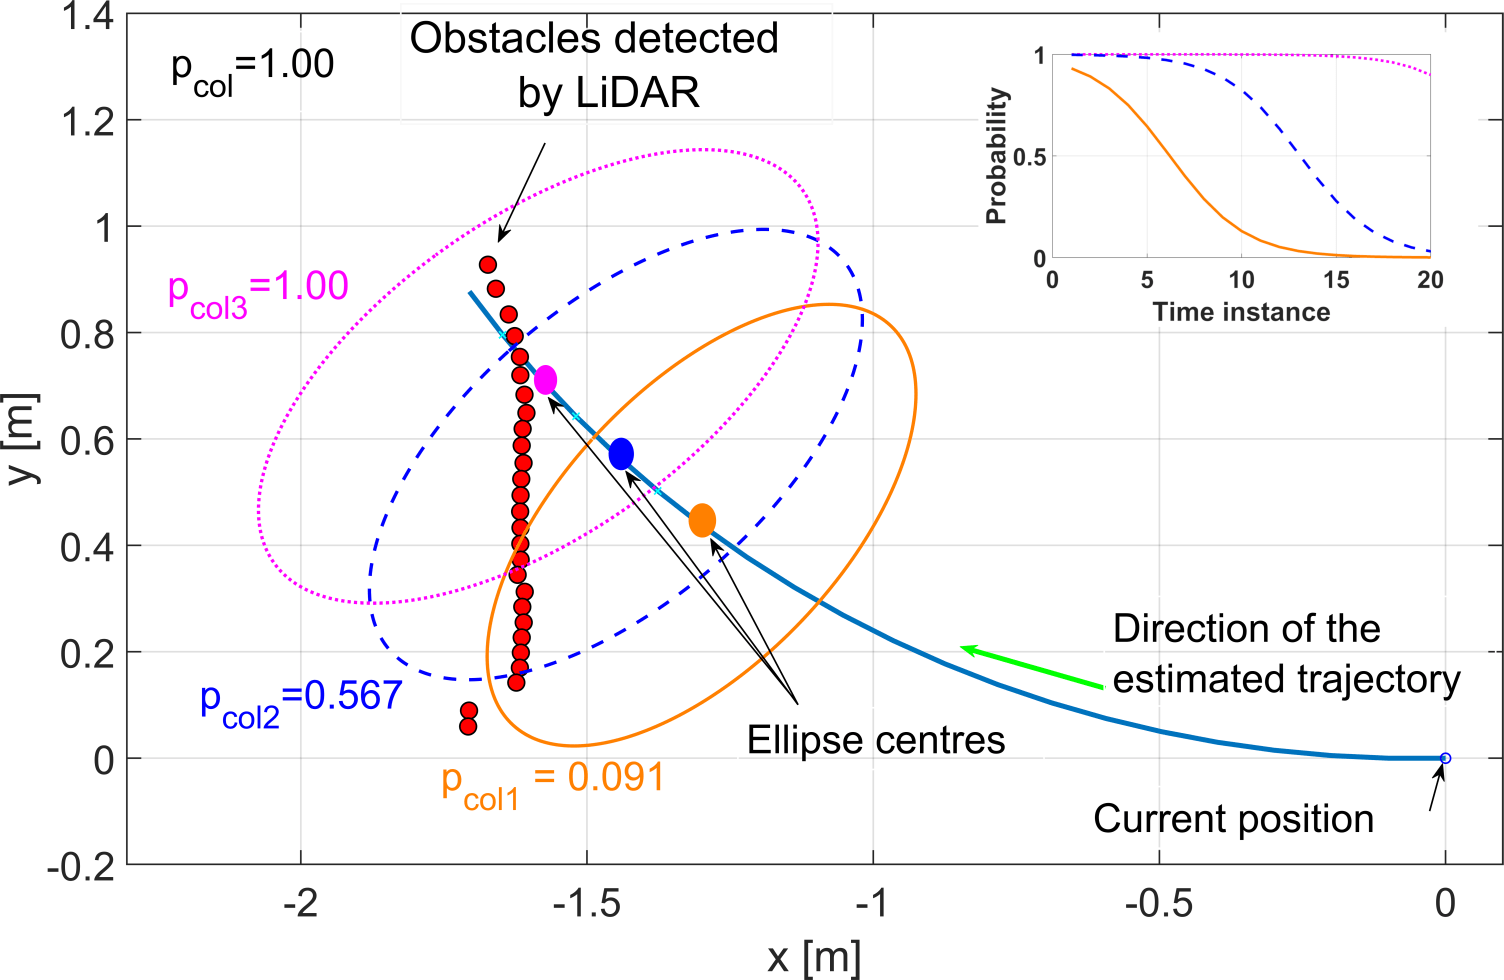
\includegraphics[width=\columnwidth]{slike/Fig03_12.png}
    \caption{An example of the collision probability calculation based on LiDAR data.}
    \label{Fig:Elipse2}
\end{figure}

After the projected trajectory has been calculated, an uncertainty ellipse is constructed around each point on the trajectory. The ellipses have increasing axes lengths with each time instance in order to account for motion uncertainty. While this always positive increase might be considered too cautious in some instances (e.g. driving parallel with an obstacle/wall), it is a prudent step since, in general, such situations where robots drive perfectly parallel to an obstacle are not too common. Also, with the appropriate selection of the initial ellipse dimensions as well as their increments (concerning the distance used in neural network-based obstacle avoidance training), this should not pose a serious limitation on robot performance (i.e. robot trajectory might be slightly longer, but the final objective would still be achieved). Ellipses' initial axis lengths and increments were determined experimentally but may change if the situation warrants it. For example, during the testing with Turtlebot 2 mobile robot, the following ellipse parameters values were used: $a_{init} = 0.3$ m, $b_{init} = 0.1$ m, $a_{incr} = 0.01$ m, and $b_{incr} = 0.005$ m (note that the $a$ axis is perpendicular to the current robot orientation). This in turn (after 2 sec ahead in time projection, as explained later on) gives an ellipse with maximum dimensions of $a_{max} = 0.5$ m and $b_{max} = 0.2$ m (keep in mind that the robot base dimensions are of 0.36 m diameter, as depicted in Figure \ref{fig:Fig08}). One possible improvement is to adjust these parameters adaptively (online). However, it should be noted that although two mobile robot platforms with very different footprints (both in size and in shape) have been used, only a limited number of parameters related to mediation were adjusted. Moreover, LiDAR readings were adjusted to better accommodate for LiDAR placement on the robot, as will be explained in more detail in Section \ref{sec:MediationExperiment}. 

An example of an estimated robot trajectory including uncertainty ellipses is shown in Figure \ref{Fig:Elipse2}. Please note that in the figure, for clarity reasons, not all ellipses are included. 

It should be noted that the time horizon was incorporated into the approach twice: through increasing uncertainty ellipses' dimensions and during the collision probability calculation (as will be explained in more detail below). However, this was done for different reasons as it was more of a binary type decision (i.e. thresholding for improved computational efficiency). At the same time, for collision probability, the points that passed the time horizon threshold were used for a more precise (fine-grained) calculation of their contribution to the final collision probability.

Once estimated trajectory and uncertainty ellipses are constructed, in the next step, each ellipse is examined to find if any parts of obstacles (i.e. LiDAR points) are located within it. If they are, the ellipse is considered further or is otherwise discarded. Then, the collision probability is estimated using a sigmoid function with variable parameters (depending on distance to the obstacle and the distance in estimation time horizon). Examples of sigmoid functions are included in Figure \ref{Fig:Elipse2}. 

The general sigmoid function that was used in the work for calculation of collision probability for time instance $i$ is derived from logistic sigmoid, defined in \cref{eq:Sigmoid} and relates to obstacle in the the form of:
\begin{equation}
    p_{\textrm{COL}\,i} = \frac{1}{1+e^{-a(i-c)}}
    \label{eq:CollisionProbability}
\end{equation}
where $a$ is a constant with a value of -0.25 (determined experimentally), $i\in[1,20]$ is the time instance for which the collision probability is calculated, and $c$ is the indicator of distance between the obstacle $(x_O,y_O)$ and estimated robot pose $(x_{R,i},y_{R,i})$ at time instance $i$ defined as
\[
    c=\frac{16}{\sqrt{(x_O-x_{R,i})^2+(y_O-y_{R,i})^2}}
\]
Please note the following:

\begin{itemize}
    \item The maximum value a sigmoid function (i.e. collision probability) can obtain is $1.0$ (or $100\%$). The function value is calculated for twenty instances, but only the value at $i$-th instance is taken into account for the collision probability calculation
    \item Parameter $a$ has a negative sign making the function open to the left. This parameter also defines the sigmoid slope (higher values give a steeper slope and vice versa).
    \item The term in the parentheses $i-c$ for a constant $a$ defines the rate of convergence of the end parts of the function (e.g. see sigmoid plots in the upper right corner of \cref{Fig:Elipse2}). In this manner, the shape of the sigmoid function (and consequently the value of the collision probability) is adaptively changed to accommodate longer time horizons in estimation (time-variable) and proximity to obstacles (distance variable). This adaptive change in sigmoid function is depicted in Figure \ref{Fig:Elipse2} alongside with related ellipses and the robot trajectory.
    \item In this manner, a maximum of $20j$ collision probabilities are calculated (where $j$ is the number of obstacles detected). If no collision probability is calculated (i.e., there are no obstacles), its value is considered 0.
\end{itemize}

Finally, when the collision probability values are calculated for each remaining ellipse, the highest collision probability is kept for that time instance. It is then used for the mediator block as the decision variable ($p_{\textrm{COL}}$) in the fuzzy set theory. Membership function was constructed in the manner depicted in Figure \ref{Fig:Fuzzy} and included five possible memberships:  \emph{no avoidance} (NA), \emph{light avoidance} (LA), \emph{balanced avoidance} (BA), \emph{strong avoidance} (SA), and \emph{full avoidance} (FA). Thus, based on the calculated collision probability for time instance $i$ ($p_{\textrm{COL}\,i}$), probabilities of belonging to each of the membership sets are calculated. 

\begin{figure}
    \centering
    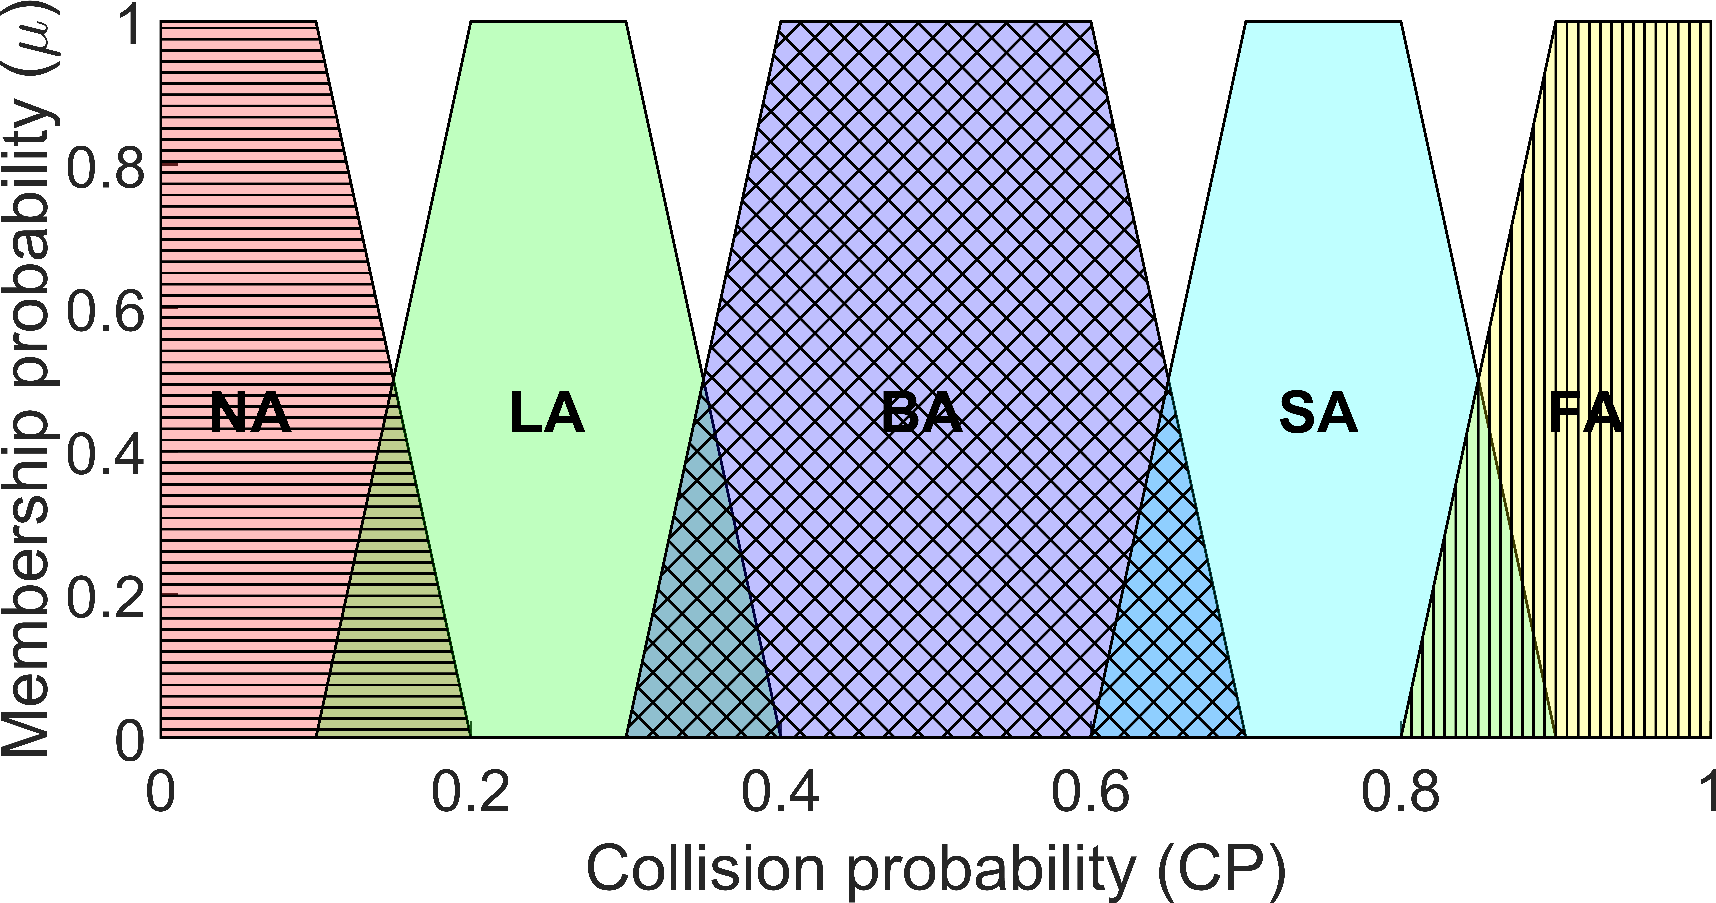
\includegraphics[width=0.75\textwidth]{slike/Fig03_13.png}
    \caption{The fuzzy set membership function used in the calculation of mediation coefficient $\zeta$.} 
    \label{Fig:Fuzzy}
\end{figure}

Each of the previously mentioned sets has its control shift factor, which is then used to compute the final output: 0, 0.25, 0.5, 0.75, and 1, respectively. These control shift factors imply that the mediation had a linear \textit{mediation engine}, but other mediation engines (like exponential ones) can be used as is pointed out in \cite{Vincenti2009}. Thus, the shift percentage is computed as
\[
    \SP_i = \SP_\NA \, \mu_{\NA\,i} + \SP_\LA \, \mu_{\LA\,i} + \SP_\BA \, \mu_{\BA\,i} + \SP_\SA \, \mu_{\SA\,i} + \SP_\FA \, \mu_{\FA\,i}
\]
where $\mu_{\textrm{XX}\,i}$ is a set membership function for the respective group at time instance $i$, and $\SP_{\textrm{XX}\,i}$ is a shift percentage for the particular set. Then the value of the calculated $\SP_i$ is used as the threshold in the Equation
\begin{equation}
    \label{Eq:zeta_SP}
    \zeta_{i} =
    \begin{cases}
    \min(1, \zeta_{i-1}+0.35), & \SP_i\geq 0.2 \\
    \max(0, \zeta_{i-1}-0.15), & \SP_i < 0.2
    \end{cases}
\end{equation}
where $\zeta_i$ is mediation coefficient used for calculation of mediated linear and angular velocities at time instance $i$, using the equation (time instance $i$ dropped for clarity reasons, since all quantities pertain to the present time instance)
\begin{equation}
    \begin{split}
     v = v_\textrm{A}\zeta + v_\textrm{N}(1-\zeta)\\
    \omega = \omega_\textrm{A}\zeta + \omega_\textrm{N}(1-\zeta)
    \end{split}
    \label{Eq:zeta}
\end{equation}

In Equation (\ref{Eq:zeta}) $v$ and $\omega$ are mediated linear and angular velocities at present instance, $v_A$ and $v_N$ are linear velocities coming from obstacle avoidance and navigation controllers, respectively, $\omega_A$ and $\omega_N$ are angular velocities coming from obstacle avoidance and navigation controller, respectively (all for the present time instance). The values of $\zeta$ are then low-pass filtered to avoid sudden changes. In the current experiments, the calculated linear velocity $v$ was not directly sent to the motor controller but was instead used for input to simple relay-type non-linearity, which produced two values at its output: slow (0.1 m/s) or fast (0.2 m/s) velocity. In Equation (\ref{Eq:zeta_SP}), increase and decrease coefficients were determined experimentally and were chosen such that the mediation swings towards obstacle avoidance more quickly than it returns to navigation since obstacle avoidance had higher priority. 

It was observed during the experimentation that the coefficients used in \cref{Eq:zeta_SP} dominantly depend on the maximal allowed linear and angular velocities (and not the robot itself, although the robot footprint was taken into account with LiDAR adjustments described in \cref{sec:MediationExperiment}). As a side note, note that in \cref{Eq:zeta_SP}, calculated collision probability value could potentially be directly used for thresholding (circumventing fuzzy set approach), but in practical testing, this proved to be too sensitive to the estimated trajectory changes (uncertainties). Additionally, since collision probability does not need to be used as a decision variable (e.g. when a different task is considered), removing fuzzy sets would reduce the generality of the proposed approach and the possibility of using nonlinear control shift functions. 

Here we demonstrate the whole calculation procedure on a simple example. Assume that the robot is going toward the goal point with a linear velocity of $v=0.2$ m/s and angular velocity of $\omega = 0.8$ rad/s. At a certain point in time $i$, the robot starts to get close to an obstacle. Thus the collision probability parameter starts to change and has a value of $p_{\textrm{COL}\,i}=0.65$. Based on Figure \ref{Fig:Fuzzy} the fuzzy set membership functions would be: $\mu_{\NA\,i}=0$, $\mu_{\LA\,i}=0$, $\mu_{\BA\,i}=0.5$, $\mu_{\SA\,i}=0.5$, and $\mu_{\FA\,i}=0$, thus the shift percentage $\SP_i$, based on \cref{Eq:zeta_SP}, would be 0.625. This value of shift percentage would result in an increase of mediation coefficient from $\zeta_{i-1} = 0$ (i.e. the robot was only navigating and did not sense any obstacle in its way) to a new value of $\zeta_i=0.35$. If we assume that the outputs from navigation controller are $v_N = 0.2$ m/s and $\omega_N = 0$ rad/s, and from obstacle avoidance $v_A = 0.2$ m/s and $\omega_A = -2$ rad/s, then based on \cref{Eq:zeta} the mediated outputs would be $v = 0.2$ m/s (not taking into account the above mentioned threshold) and $\omega = -0.18$ rad/s. From the example, the main idea of the work can be seen. Namely, since the collision probability is detected (based on the current linear and angular velocity, 0.2 m/s and 0.8 rad/s), the mediation mechanism now considers the obstacle avoidance controller. It shifts the control values in its favour (for the angular velocity from 0.8 rad/s to -0.18 rad/s). If the collision probability persisted, then this move would, in the next time instance, be even more in favour of the obstacle avoidance algorithm, but if not, it would slowly return control to the navigation controller.

\subsection{Experimental Setup}
\label{sec:MediationExperiment}

The experimental verification and testing of the proposed approach consisted of three main parts: simulation-based, real-world based, and application-specific. The main idea behind each of them was as follows. The goal of the simulation experiment was to initially verify the functioning and viability of the proposed approach, while the goal of the real-world experiment was to build upon the simulation experiment and demonstrate that the approach is valid on real robots with different footprints and indifferent (realistic) situations. Finally, the application-specific testing aimed to demonstrate that the proposed approach could be of practical use for solving or minimising some of the real-world problems (teleoperation was chosen as one such problem). 
In all three cases, neural networks were used for obstacle avoidance (as described in detail in Section \ref{sec:MMAvoidance}). These networks, along with other controllers, mediation and all other algorithms, were deployed in ROS environment, which made (in some cases) running the system in a distributed manner possible (i.e. neural network was running on a separate computer due to hardware resource-related issues).

\subsubsection{Simulation} \label{sec:MediationSimulation}
Simulation experiments were carried out in the Gazebo 7 simulation environment. During this test, a random environment was generated with randomly distributed obstacles of different shapes (cylinders of 0.5 m diameter and cubes with a side length of 0.5 m). An example of the simulation environment used for testing is depicted in Figure \ref{Fig:Gazebo3D}. Note that the overlap of obstacles was permitted.

\begin{figure}
\centering
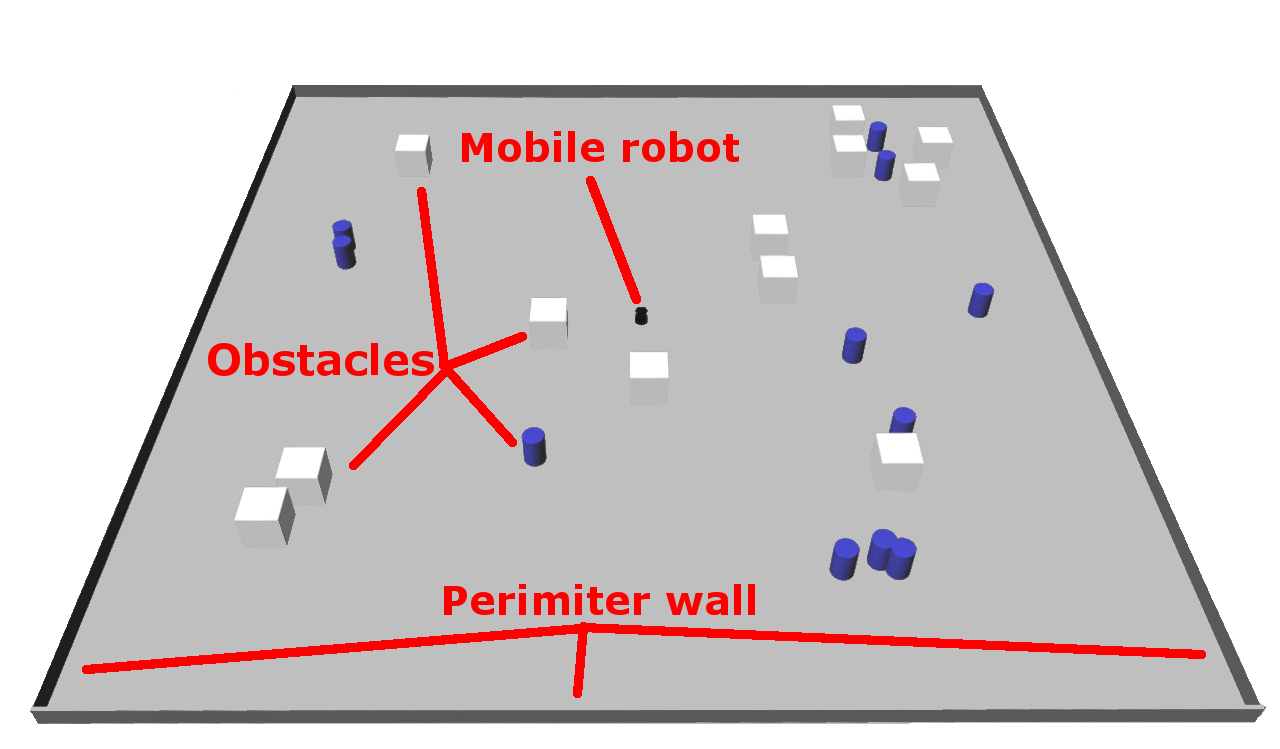
\includegraphics[width=0.7\columnwidth]{slike/Fig03_14.png}
\caption{Gazebo simulation environment used for testing of the fuzzy mediation approach}
\label{Fig:Gazebo3D}
\end{figure}

The random environment generated during the testing had a fixed size (defined by a perimeter wall) of 25 m $\times$ 25 m and a fixed number of obstacles within it (24, out of which 12 were cylinders and 12 were cubes). This number of obstacles was chosen since it provided a sufficiently challenging environment while not being too cluttered (please keep in mind that the focus of the research was the fuzzy mediation algorithm as a whole and not the obstacle avoidance alone). Fifteen runs were executed in the environment for each navigation controller (P-type controller and neural networks-based controller presented in \cref{sec:MMMediationFormulation}), giving 30 simulation runs. In all runs, neural network-based obstacle avoidance was used (presented in \cref{sec:MMAvoidance}). In each run, the robot started from the same position (centre of the environment) and with the same orientation (looking down in Figure \ref{Fig:Gazebo3D}) and had to navigate to a randomly given point in the environment, with the map not being available. No time limit was given, and the trajectory and outcome (success or crash) were recorded. Results of this experiment are reported in Section \ref{sec:MediationSimResults}.

\subsubsection{Simple real-world scenarios} \label{sec:MediationReal}
Real-world experiments were carried in the indoor environment at the Faculty of Electrical Engineering, Mechanical Engineering, and Naval Architecture, University of Split. During the experiments, two mobile robot platforms with very different footprints, masses and characteristics were used: customised Turtlebot 2 depicted in Figure \ref{fig:Fig08} weighing about 10 kg, and a custom-built mobile platform intended to be used as an automated pallet carrier depicted in Figure \ref{Fig:paletarCombo}, weighing about 100 kg. Please note that raw LiDAR data was not fed to the neural network-based obstacle avoidance but rather an adjusted one in the case of a custom-built robot. The adjustment was achieved by simply adding/subtracting from the measured distance (in an online manner), which took into account robot footprint and sensor placement within it (i.e., LiDAR scans were transformed to the robot centre) to be in line with the one used for the training of the neural networks. Of course, if the training were achieved with a different/actual footprint, this step would not be needed, but it shows how the approach can be extended to work with different robots.

\begin{figure}
\centering
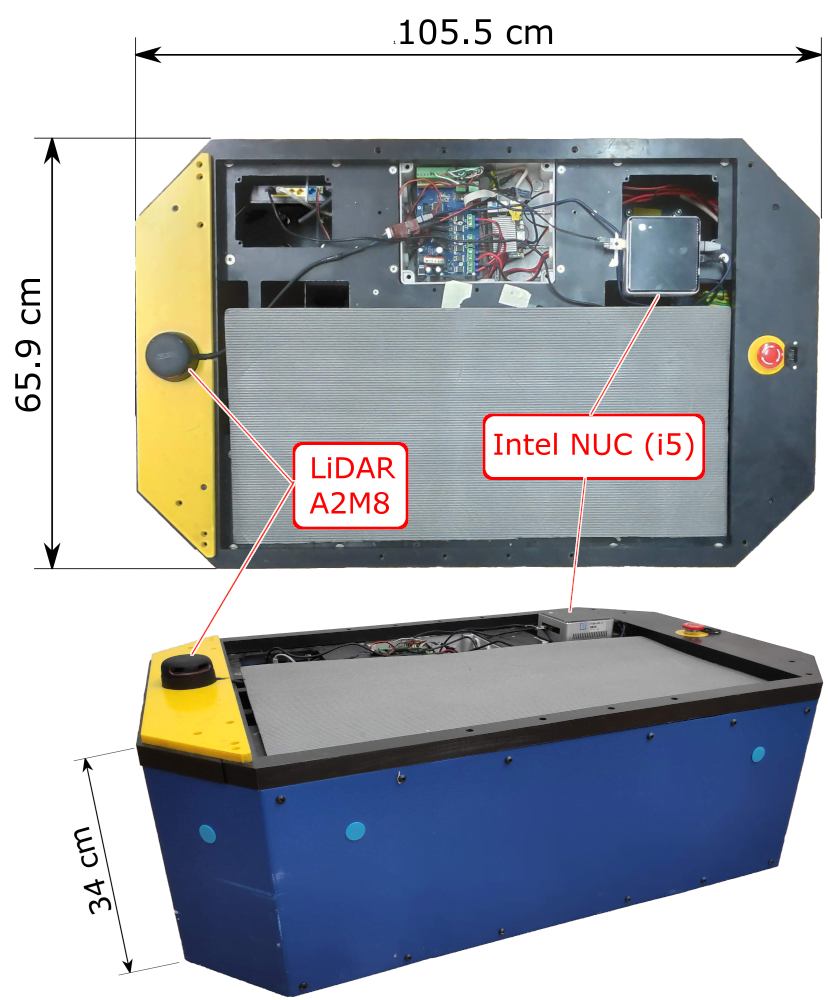
\includegraphics[width=0.6\textwidth]{slike/Fig03_15.png}
\caption[Overview of a custom-built robot]{Overview of a custom-built robot (built by our project partner ``Statim'')}
\label{Fig:paletarCombo}
\end{figure}

The main idea behind using such different mobile bases was to demonstrate the effectiveness and generalisation of our mediation approach. This idea is essential since several parameters are needed for the approach (as described in Section \ref{sec:MMMediation}), and the question of generality (i.e. the need for fine-tuning them) naturally arises. As will be discussed later on in Section \ref{sec:MediationRWResults} it was found that it is sufficient to fine-tune only two parameters, those related to uncertainty ellipses, to ensure the desired behaviour of the mobile robot. Fine-tuning other parameters could improve the performance, but optimisation was not in focus.

Next, two main test scenarios were devised for each of the mobile bases. First, for Turtlebot 2, the experiments consisted of three distinct navigation and obstacle avoidance tasks. In all three cases, three setups were used: proposed approach with neural network-based navigation and with P controller navigation (both with neural network-based obstacle avoidance), as well as the default method in ROS navigation stack, which is based on DWA for obstacle avoidance and Dijkstra for navigation as a baseline method. The first two tasks were conducted in an environment augmented with Z- and U-shaped \footnote{This U-shaped obstacle is different from one used in the obstacle avoidance experiment} (convex dead-end) obstacles. Five instances of these tasks were run per each setup (15 in total). The final task was navigation in a large real-world environment with two distinct navigation goals - 2 examples, and it was run once per setup (6 runs in total). The real-world experiments were conducted in the atriums and corridors in the Faculty building.

The same test cases (Z- and U- shape tests) could not be used for the custom-built robot due to its larger size. Thus, the testing was slightly modified. Firstly, a test course was constructed (as depicted in \cref{fig:PaletarB401}) within which the robot had to reach (from the same starting position and orientation) three different goals (the final orientation was not essential). Since three setups were used (neural network-based navigation and P-type controller -- both with neural network-based obstacle avoidance and ROS navigation stack), 9 test runs were recorded. The distance between the starting point and goal point ranged from about 10 m to about 16 m (measured in a straight line).

\begin{figure}
    \centering
    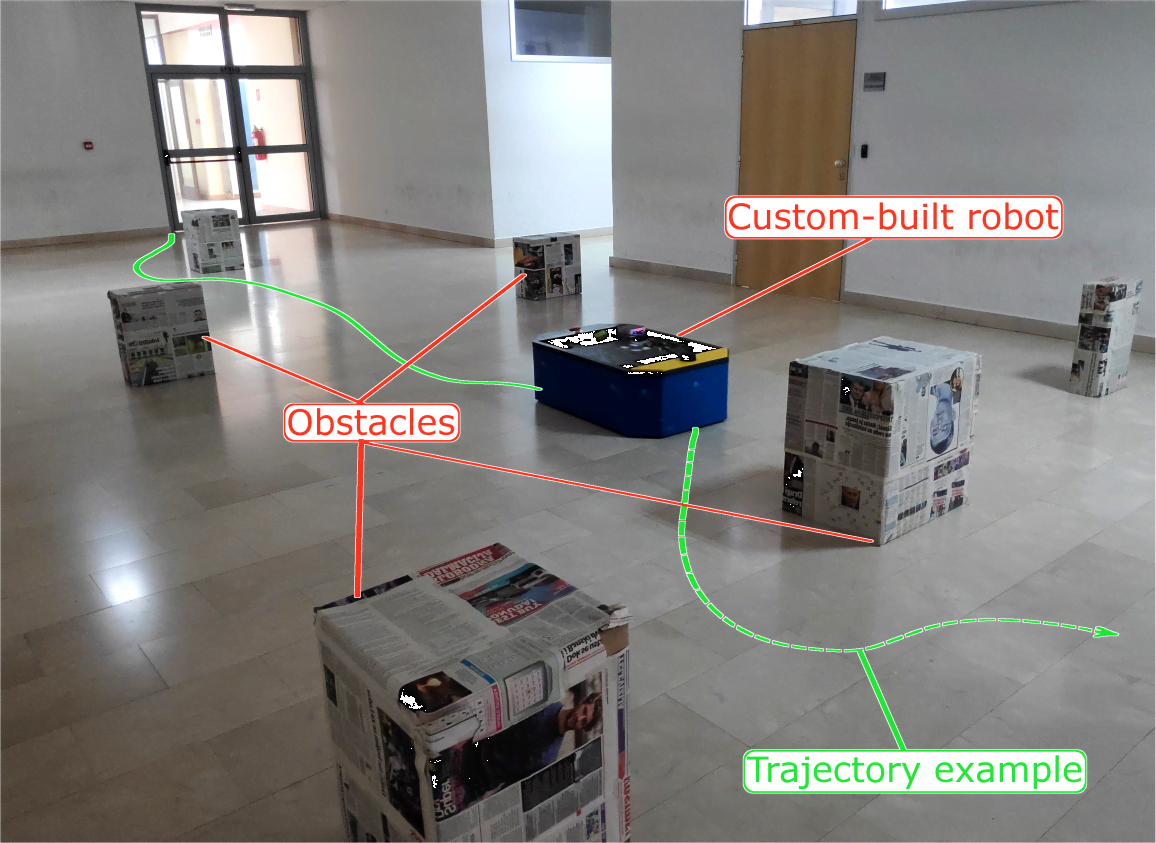
\includegraphics[width=0.8\textwidth]{slike/Fig03_16.png}
    \caption{Test course for the custom-built robot}
    \label{fig:PaletarB401}
\end{figure}

Next, the same larger environment for real-life testing was used for both Turtlebot 2 and the custom-built robot (with the same goal points, except that the goal circle was enlarged so that the bigger robot could more easily meet termination conditions). During this testing, simplified path planning and line following algorithm was introduced (as a fourth test case, but just in case of the custom-built robot) so that three additional waypoints could be given to the algorithm, and they were connected with straight lines (possible even through walls). The area where the experiment was conducted is shown in \cref{fig:FESB4kat} with marked start and goal points. This test was introduced to assess if the approach could be integrated with a simplified path planning algorithm within an arbitrary navigation approach and test if the addition of waypoints could improve the performance of mediated navigation. Results obtained for all mentioned cases are presented in Section \ref{sec:MediationRWResults}.

\begin{figure}
    \centering
    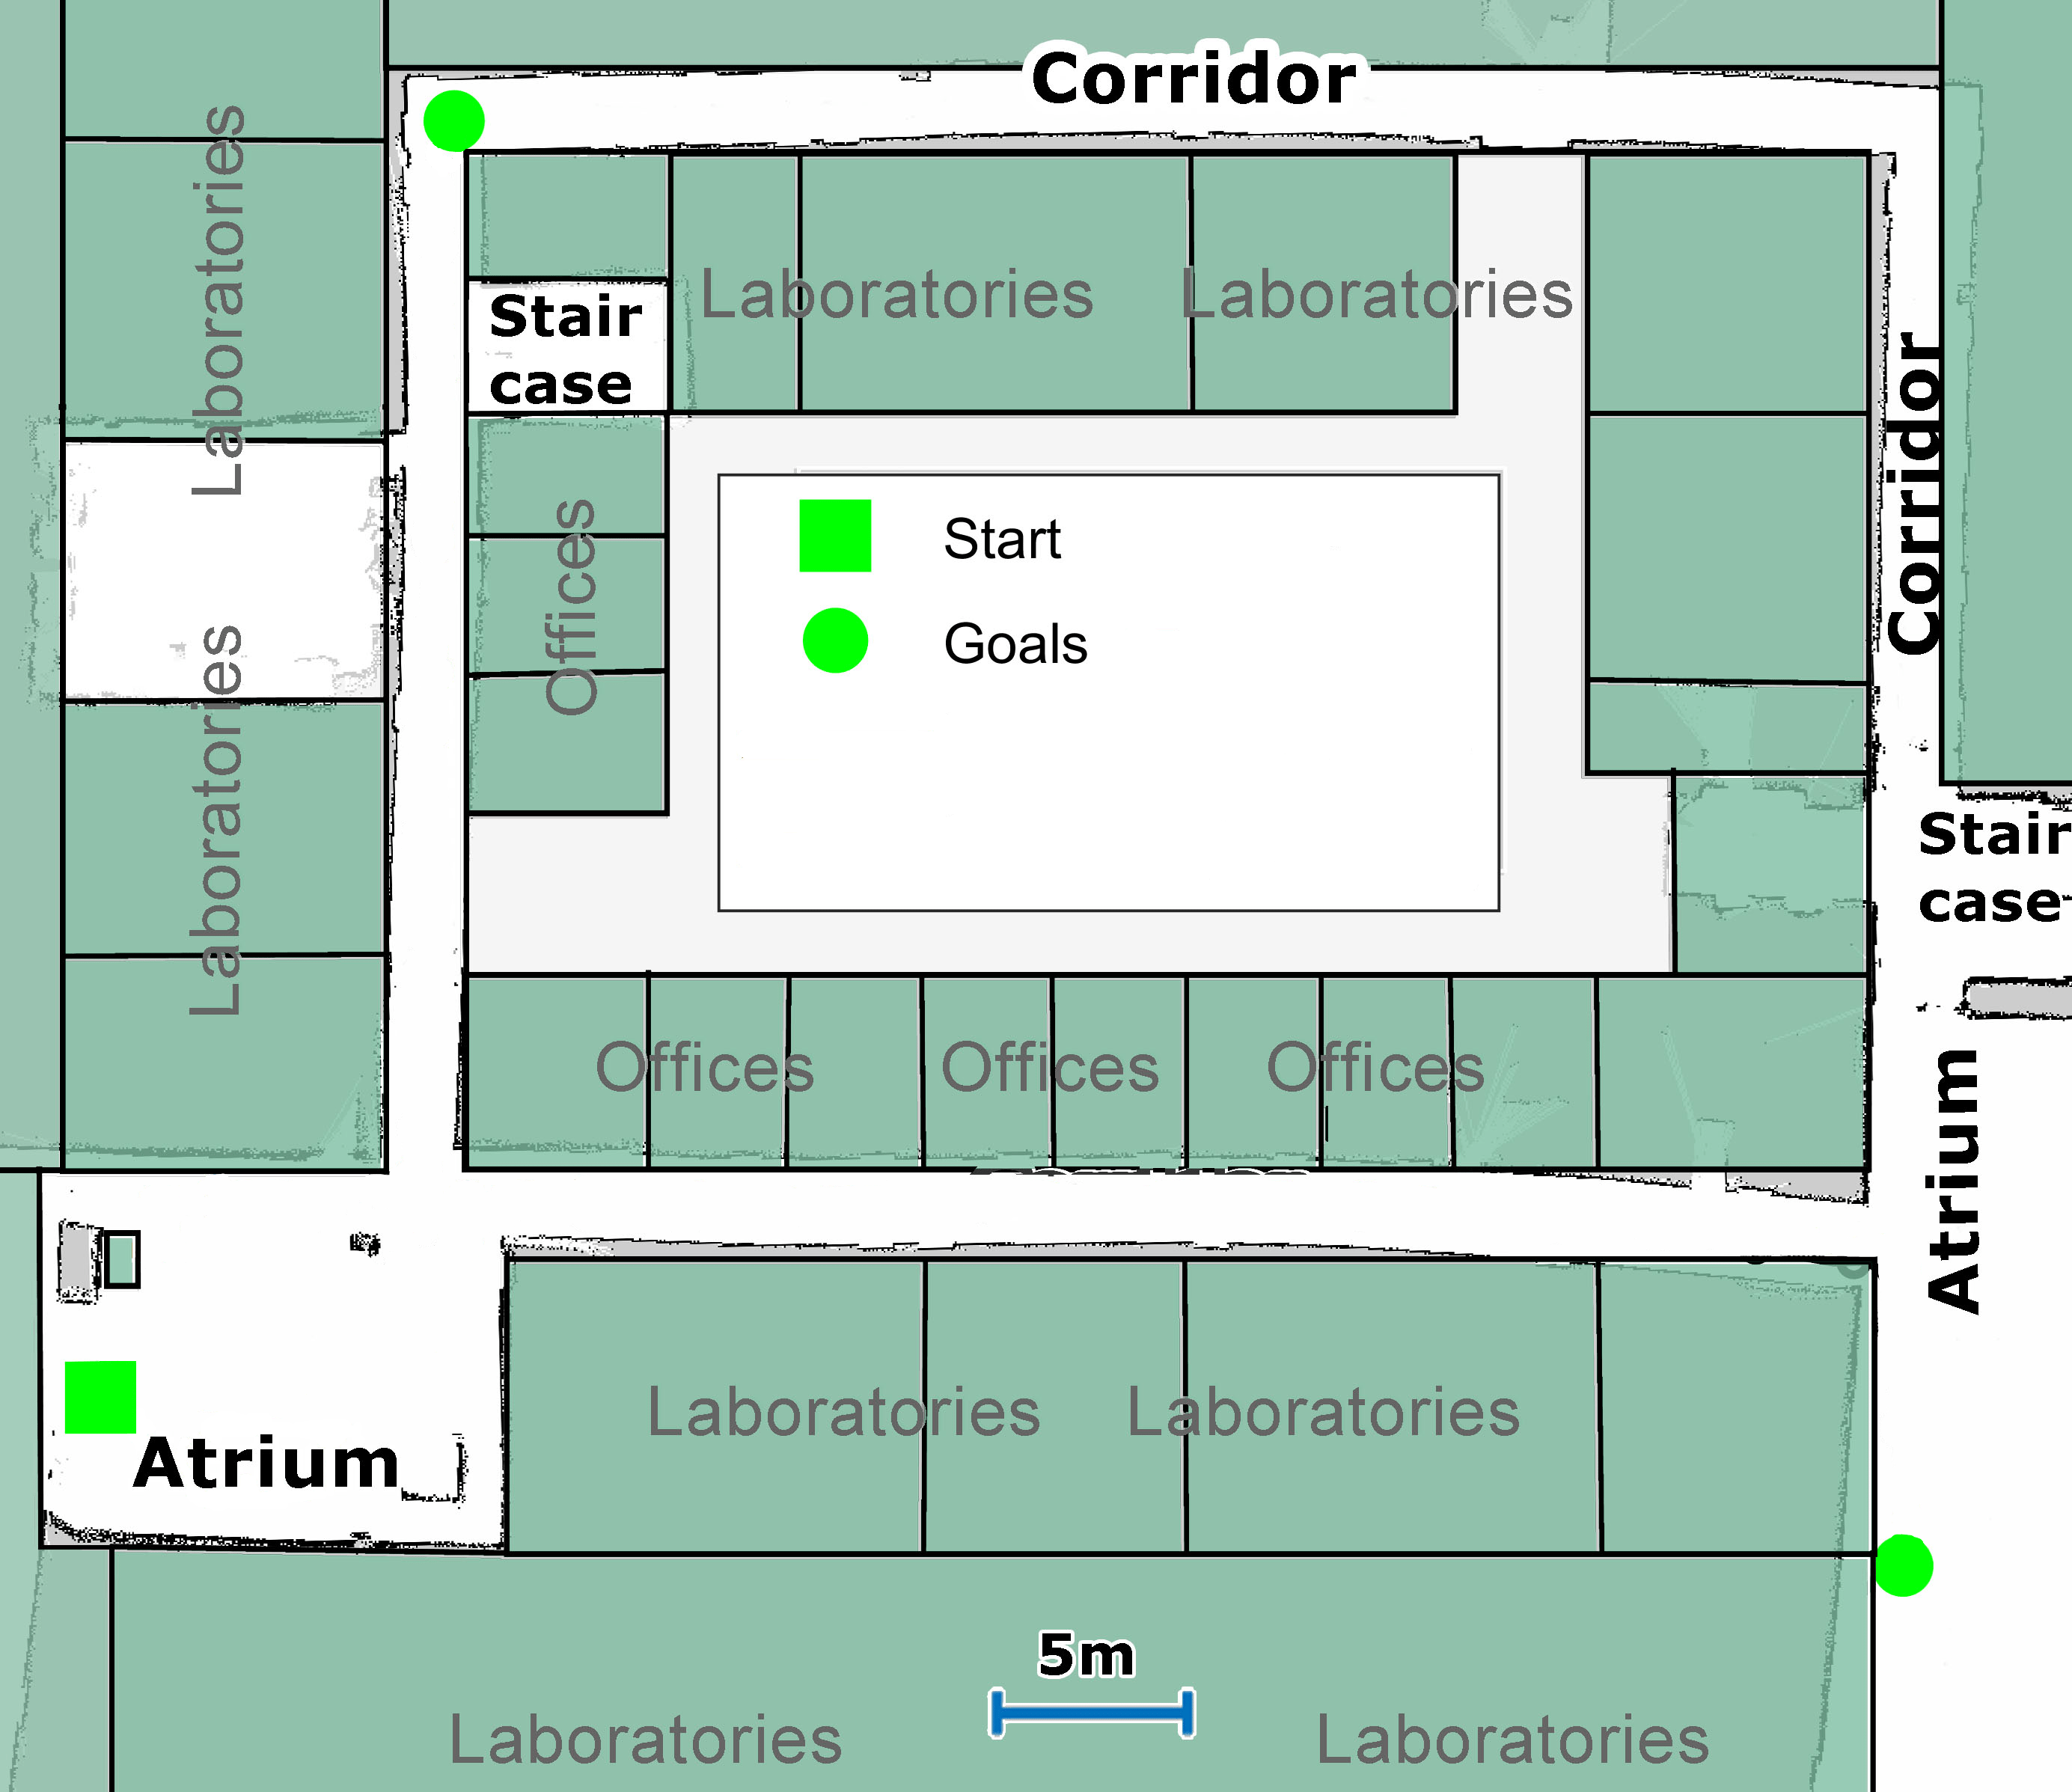
\includegraphics[width=0.85\textwidth]{slike/Fig03_17.png}
    \caption{Real-world experimental area}
    \label{fig:FESB4kat}
\end{figure}

\subsubsection{Teleoperation scenario}
\label{sec:MediationApp}

The purpose of the final test scenario was to demonstrate the practical applicability of the proposed approach. Thus a simple teleoperation scenario was envisaged in which users had to avoid a single obstacle and reach a goal point. Teleoperation was chosen since it lends itself as a natural testing ground for automatic obstacle avoidance and human-robot interaction approaches. An overview of this simple experimental setup is depicted in Figure \ref{Fig:tele2Course}.

\begin{figure}
\centering
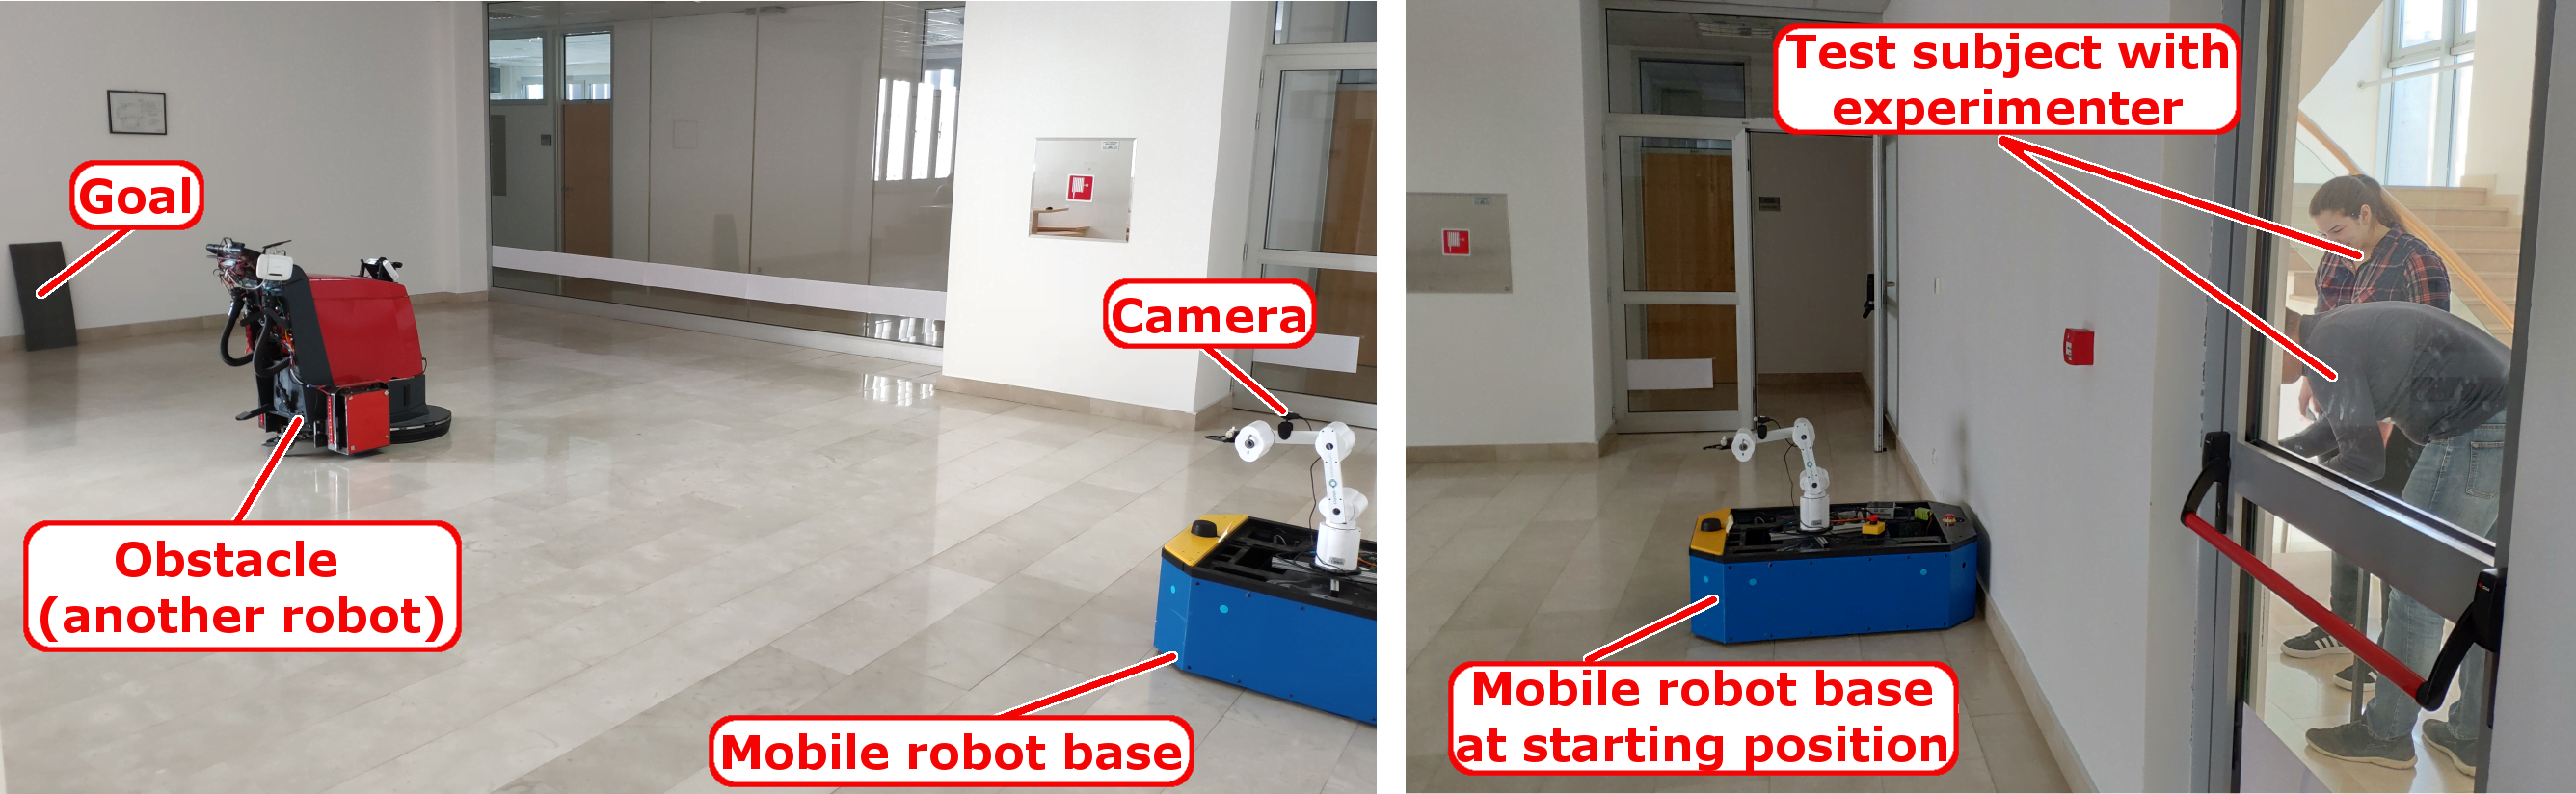
\includegraphics[width=1\columnwidth]{slike/Fig03_18.png}
\caption{Overview of a simple teleoperation scenario used in the experiment.}
\label{Fig:tele2Course}
\end{figure}

A total of 9 test subjects (three females and six males) participated in the mini-study. The mean age of the test subjects was 32.78 with the standard deviation of $\pm$10.52 years. The test subjects were students and staff of the Faculty (note that no staff was involved in the development of the experiment). Out of all test subjects, four (44 \%) had some previous experience with teleoperation.
Test subjects were informed about the study's goal and the remote controller setup used for controlling the robot. The test subjects were placed in a different room than a mobile robot (as depicted in Figure \ref{Fig:tele2Course}), and the only feedback they had from a robot was a video stream coming from the camera mounted on a mobile base system (Manhattan Webcam 500, having 55$^{\circ}$ horizontal viewing angle, and running in 25 fps with resolution set to 680x480). The camera was positioned so that the area near the front of the mobile base was not visible. This kind of camera positioning was done to simulate the lack of situational awareness during teleoperation. The robot was running the proposed mediation algorithm, in which neural network-based obstacle avoidance was one input to the mediator and human controller input the other one. If the user were too close to an obstacle, the neural network-based obstacle avoidance would gradually (depending on collision probability value) take over the control, steer it from danger, and (gradually) give back the control to the user. Users were informed that two cases would occur (in random order): \emph{\textbf{no} unexpected obstacles case} and \emph{unplanned obstacles case} (thrown in front of the mobile robot by a second experimenter in such a manner that the camera cannot easily see it). This procedure was repeated several times, and collision/non-collision events were recorded. Furthermore, at the end of the test runs, each user had to fill out a simple questionnaire (and share her/his experience in a free-form interview) with the following questions (other questions not reported here pertained to demographics):

\begin{enumerate}
\item Did you feel in full control during the teleoperation?
\item Do you feel that automatic obstacle avoidance through mediation helped you during teleoperation?
\item Was completing the required task easier with or without the mediation?
\end{enumerate}

Answers for the first two questions were on a Likert-like scale with three labelled answers (e.g. "Strongly agree", "Neutral", and "Strongly disagree") and the continuous line between them. The users had to mark a place on the line which best matched their response. These kinds of answers enabled us to obtain continuous variable data from the responses. Please note that the users were not allowed to practice the mediated teleoperation not to get accustomed to it. They were, however, free to test the remote controller and video feedback. Results for this experiment are presented in Section \ref{sec:MediationTeleopResults}.

\section{Forces and joint torques estimation}
\label{sec:MMForceEstimation}

\subsection{Problem formulation}

The measurement of the mobile robotic manipulator interaction forces, acting on the end-effector, can, in some instances, be challenging, which especially holds when robots with small payloads are used (and consequently not capable of mounting a force sensor on the robot tip). For example, this is often the case with educational robots, but also the mounting of a force sensor on the industrial robot may be inconvenient in some applications when the full payload needs to be available for regular operation.

An approach to estimating forces acting on the robot end-effector and joint-side torques is developed. The estimation is achieved by using forces measurements with a sensor mounted under the robot base. The approach has the obvious benefit of not consuming any payload. However, the force acting on the robot tip cannot be measured directly but is estimated using the measurements of the force sensor mounted below the robot base and with data about kinematics that are usually provided by the robot (joints positions and its derivatives).

The other benefits of such methods are that they do not rely on measurements of joint motor currents because forces can be directly measured using force sensors, which are generally reliable and provide very accurate measurements. Contrary to the approaches that use robot dynamics models for estimating end-effector forces and joint torques, as outlined in Chapter \ref{chap:Literature}, the proposed method uses neural networks to do the estimation. These neural network-based approaches have certain advantages. They do not require the knowledge of the robot's dynamic model (it is learnt from data implicitly) and, when deployed, is computationally cheap since once trained, neural network evaluations are fast and well-suited for real-time use.

\subsection{Data collection}

Training neural networks were collected on two robots: Commonplace Robotics Mover 6, a small six-degrees-of-freedom robot intended for education, and Franka Emika Panda, a 7 DOF industrial robot (in simulation and the real-world scenario). Although the two robots differ in shape, size, and payload, the basic outline of how the data that was collected is the same, the exact procedure depends on the robot itself. Thus, the details will be given in the following subsections for each robot separately.

Following the data collection, several datasets were created using the same measurements data. These datasets had to be created since LSTM and convolutional neural networks operate on sequential data. Thus, the datasets used to train these network architectures needed additional preprocessing steps in which input data are arranged as sequences.

\subsubsection{CPR Mover6 robot}

Commonplace Robotics Mover6 robot is a six-degree-of-freedom robot intended primarily for education \cite{Mover6} and is shown in \cref{fig:Mover6}. 

\begin{figure}
    \centering
    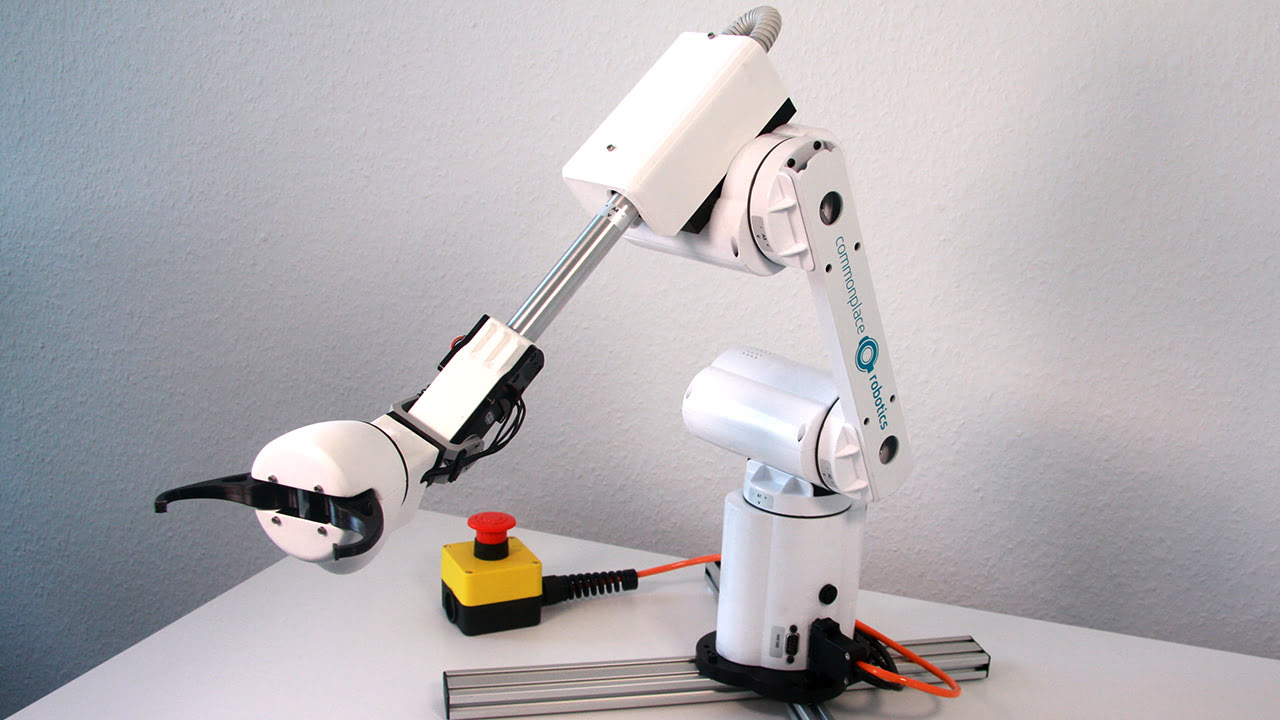
\includegraphics[width=0.75\textwidth]{slike/Fig03_19.jpg}
    \caption[Commonplace Robotics Mover6 robot]{Commonplace Robotics Mover6 robot \cite{Mover6}}
    \label{fig:Mover6}
\end{figure}

Unfortunately, the manufacturer did not provide the dynamics model or any relevant data that makes the computation of the dynamic model possible. Furthermore, the manufacturer declared that the robot has a payload of only 0.4 kg, which makes the use of wrist-mounted force sensors inconvenient due to their mass, consuming the majority of the payload. Thus, for this experiment, an auxiliary interaction tool was devised to make a direct measurement of end-effector forces possible, as depicted in Fig. \ref{fig:Tool}. The tool featured a hemispheric dome placed on the force sensor to focus forces and had Optotrak markers, based on which its orientation was determined. It was held by the experimenter who applied the force to the robot end-effector, as illustrated in Fig. \ref{fig:Robot}. 

\begin{figure}
    \centering
    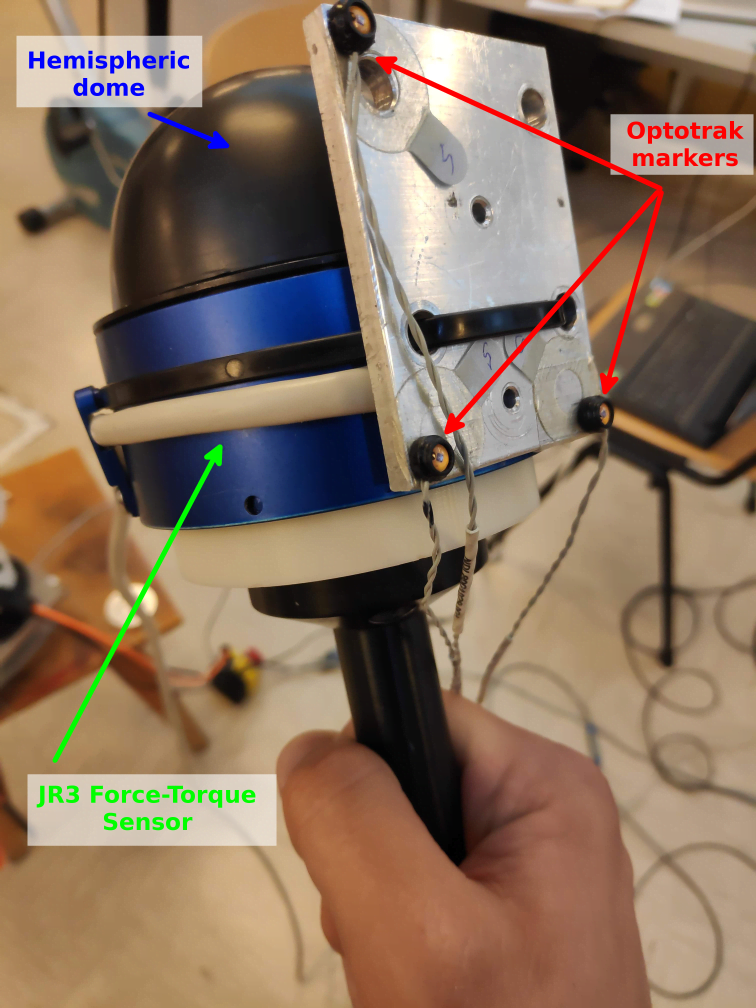
\includegraphics[width=0.5\textwidth]{slike/Fig03_20.png}
    \caption{Custom-built interaction tool used for data collection}
    \label{fig:Tool}
\end{figure}

The robot executed random valid trajectories in the process. The other force sensor was mounted below the robot base. Both sensors were JR3 90M40 6-axis force-torque sensors, and data acquisition was made using Mathworks Simulink Real-Time 2019a software which also synchronised sensors at a rate of 100 Hz. Additionally, Optotrak Certus optical motion capture system was used for assessing the positions and orientations of the robot base and the interaction tool through measuring the 3D positions of optical markers. The position data measurements were synchronised with force measurements. Robot joint positions that are provided by encoders on each of the joints were also recorded.

\begin{figure}
    \centering
    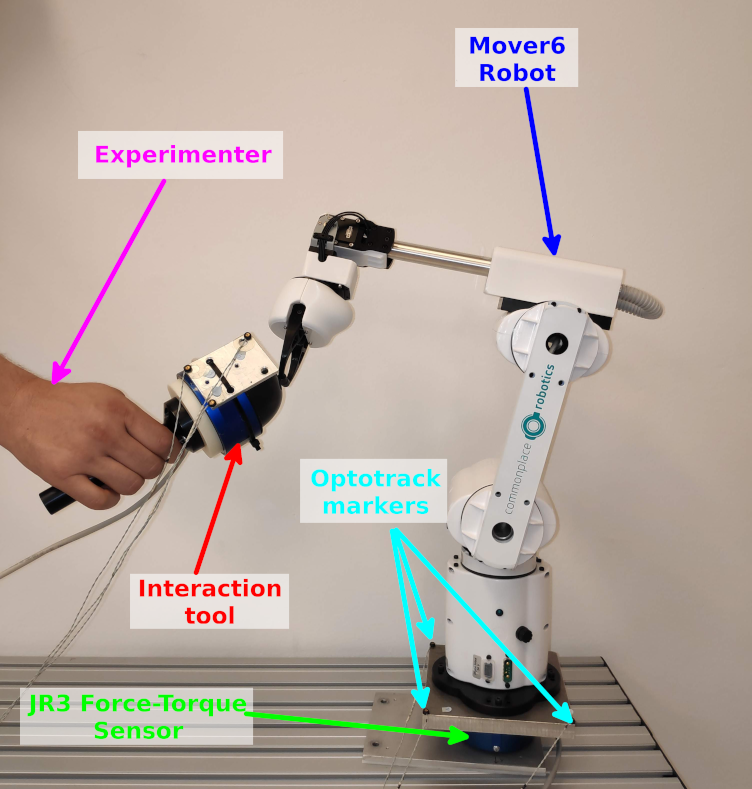
\includegraphics[width=0.6\textwidth]{slike/Fig03_21.png}
    \caption{The process of collecting measurements.}
    \label{fig:Robot}
\end{figure}

The data were collected as follows. The experimenter holding the interaction tool applied forces to the robot by making contact between the interaction tool dome and the robot end-effector while the robot was either in motion or standstill. Random valid goal positions and orientations were generated during the robot motion, and trajectories were planned and executed. Between two successive motion trajectories, the robot was, for a short time, at a standstill. A random number of up to six contacts were made in a single measurement instance, and a total of 800 measurement instances of random length, ranging from approx. 10 s to approx. 30 s were recorded, resulting in a total of 1,803,875 samples. 

Following the data collection process, before using the data for training neural networks, all obtained measurements were preprocessed so that both robot base and interaction tool forces were aligned to the same reference frame. Next, the forces were expressed in the same reference frame thanks to positions obtained from Optotrak markers; three were positioned on the robot base and three on the interaction tool, which was used to define a reference frame corresponding to the robot base the interaction tool, respectively. Following this, the transformation between the two frames was obtained and used to express both measured forces in a common reference frame so that the principal axes from both force measurements match. Finally, the obtained forces were low-pass filtered to remove noise.

\subsubsection{Franka Emika Panda robot}

Franka Emika Panda \cite{FrankaRobot} is a seven-degrees-of-freedom robotic manipulator intended for industry and research. The robot is big enough, and its payload is big enough to make mounting the force sensor on the robot tip possible. It features position, velocity and force control schemes. The data provided by the robot controller is much richer than in the case of the Mover6 robot. It contains joint positions, velocities and torques and even some data that were not used in the research and thus not recorded.

The data collection was conducted both on the real robot and in simulation. In the real world, the experimenter applied a random force to a robot tip (on which a force sensor was mounted) while the robot was either in motion, executing random but valid trajectories, or at a standstill. This experiment was similar to the Mover6 experiment, but the devised interaction tool was not used. This time, the force sensor was convenient to mount on the robot tip due to the large enough payload, and thus Optotrak markers were not used since the transformation between the robot tip and the force sensor is known and constant. Instead, the experimenter applied the force to the robot tip using their own hands (fingers) at the middle of the adapter plate mounted to the sensor. In the simulation, the data collection setup was configured similarly, but this time the experimenter was replaced by a mathematical function that generated forces randomly, but in such a way that they looked like ones from the real world. For this, a bell-shaped curve was used since it nicely accomplishes the similarity to the real world where the experimenter applied force (see \cref{fig:FextSimReal} for comparison). Thus, the external force was generally defined as:
\[
F_{ext}(t) = \sum^n_{i=1}-1^{\{0,1\}}A_i e^{-\frac{(t-\tau_i)^2}{2\sigma_i^2}}
\]
where $A_i$, $\tau_i$ and $\sigma_i$ are amplitude, time offset and standard deviation\footnote{Standard deviation defines the width of the bell-shaped curve} of the bell-shaped curve, respectively; these definitions are shown in \cref{fig:Bell}. The term $-1^{\{0,1\}}$ is a randomly generated sign. $n$ is the number of how many times the external force acts on the robot end-effector (the values were integers in the range [5, 15] per measurement instance). Amplitudes, time offsets and standard deviation are all generated randomly (ranges: [5,20] N, [5, 10] s and [0.5, 1.5] s, respectively). 

\begin{figure}
    \centering
    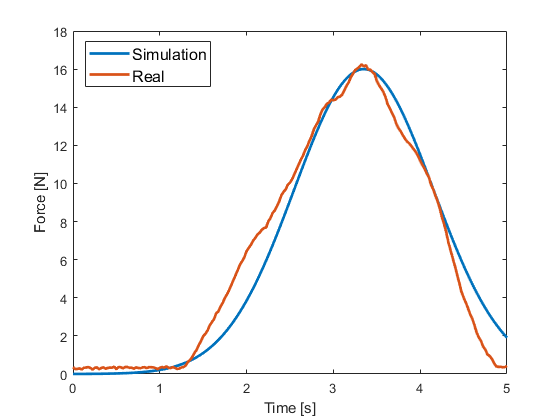
\includegraphics[width=0.8\textwidth]{slike/Fig03_22.png}
    \caption{Comparison of external forces in simulation and real world}
    \label{fig:FextSimReal}
\end{figure}

\begin{figure}
    \centering
    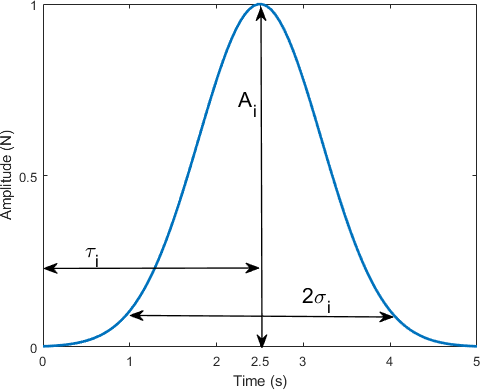
\includegraphics[width=0.7\textwidth]{slike/Fig03_23.png}
    \caption{Bell-shaped curve template used to generate external forces in simulation}
    \label{fig:Bell}
\end{figure}

The dynamic model of the robot that the simulation was based on was provided in \cite{Gaz2019}, and as a simulation environment, CoppeliaSim (formerly known as V-REP) \cite{Rohmer2013} was used.

There were 1000 measurement instances with between 5 and 50 valid trajectories executed in each. For trajectory generation, first, a valid goal was generated randomly (uniform, in joint space), then a trajectory to that goal from the present robot state was planned using Open Planning Library \cite{Sucan2012} and its default planning algorithm, the Rapidly-exploring Random Tree (RRT) Connect algorithm. If no trajectory was found, the procedure was repeated until a valid trajectory was found. Between the execution of trajectories, there was a 1-second standstill. 

The dataset was split in the following manner. The test set was created using randomly selected 20\% of data instances, while 80\% was used for training and validation purposes, from which further random 20\% (or 16\% in terms of the whole dataset) was used as a validation set. The rest was used as a training set. With this in mind, the training set consisted of 640 simulation instances, a validation set of 160 simulation instances and a test set of 200 simulation instances.

A total of 3,919,800 samples were collected, which took about 48 hours in simulation on a computer with an Intel Core i3-6100 processor with 16 GB RAM, but in practice, that was a shorter time since simulation runs faster than real-time. The simulation engine used for the simulations was provided by the CoppeliaSim environment, and it was the Newton Dynamics engine \cite{Massera2007}. The simulation step was set to 50 ms. An example of simulation running using the described experimental setup with four visualised trajectories and plotted forces on base and tip is shown in \cref{fig:Coppelia}. Please note that periods may exist without an external force acting on the end-effector during the execution of the trajectories. This way, the dataset was made more diverse in order to generalise better. 

\begin{figure}
    \centering
    \subfloat[CoppeliaSim with four visualised trajectories]{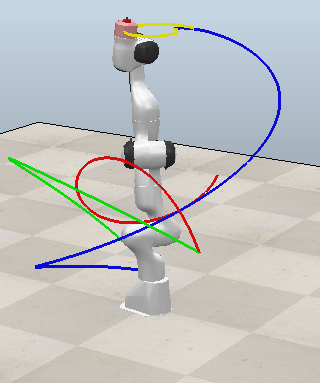
\includegraphics[width=0.35\textwidth]{slike/Fig03_24a.png}}
    \hfill
    \subfloat[Corresponding three force interactions for the visualised trajectories]{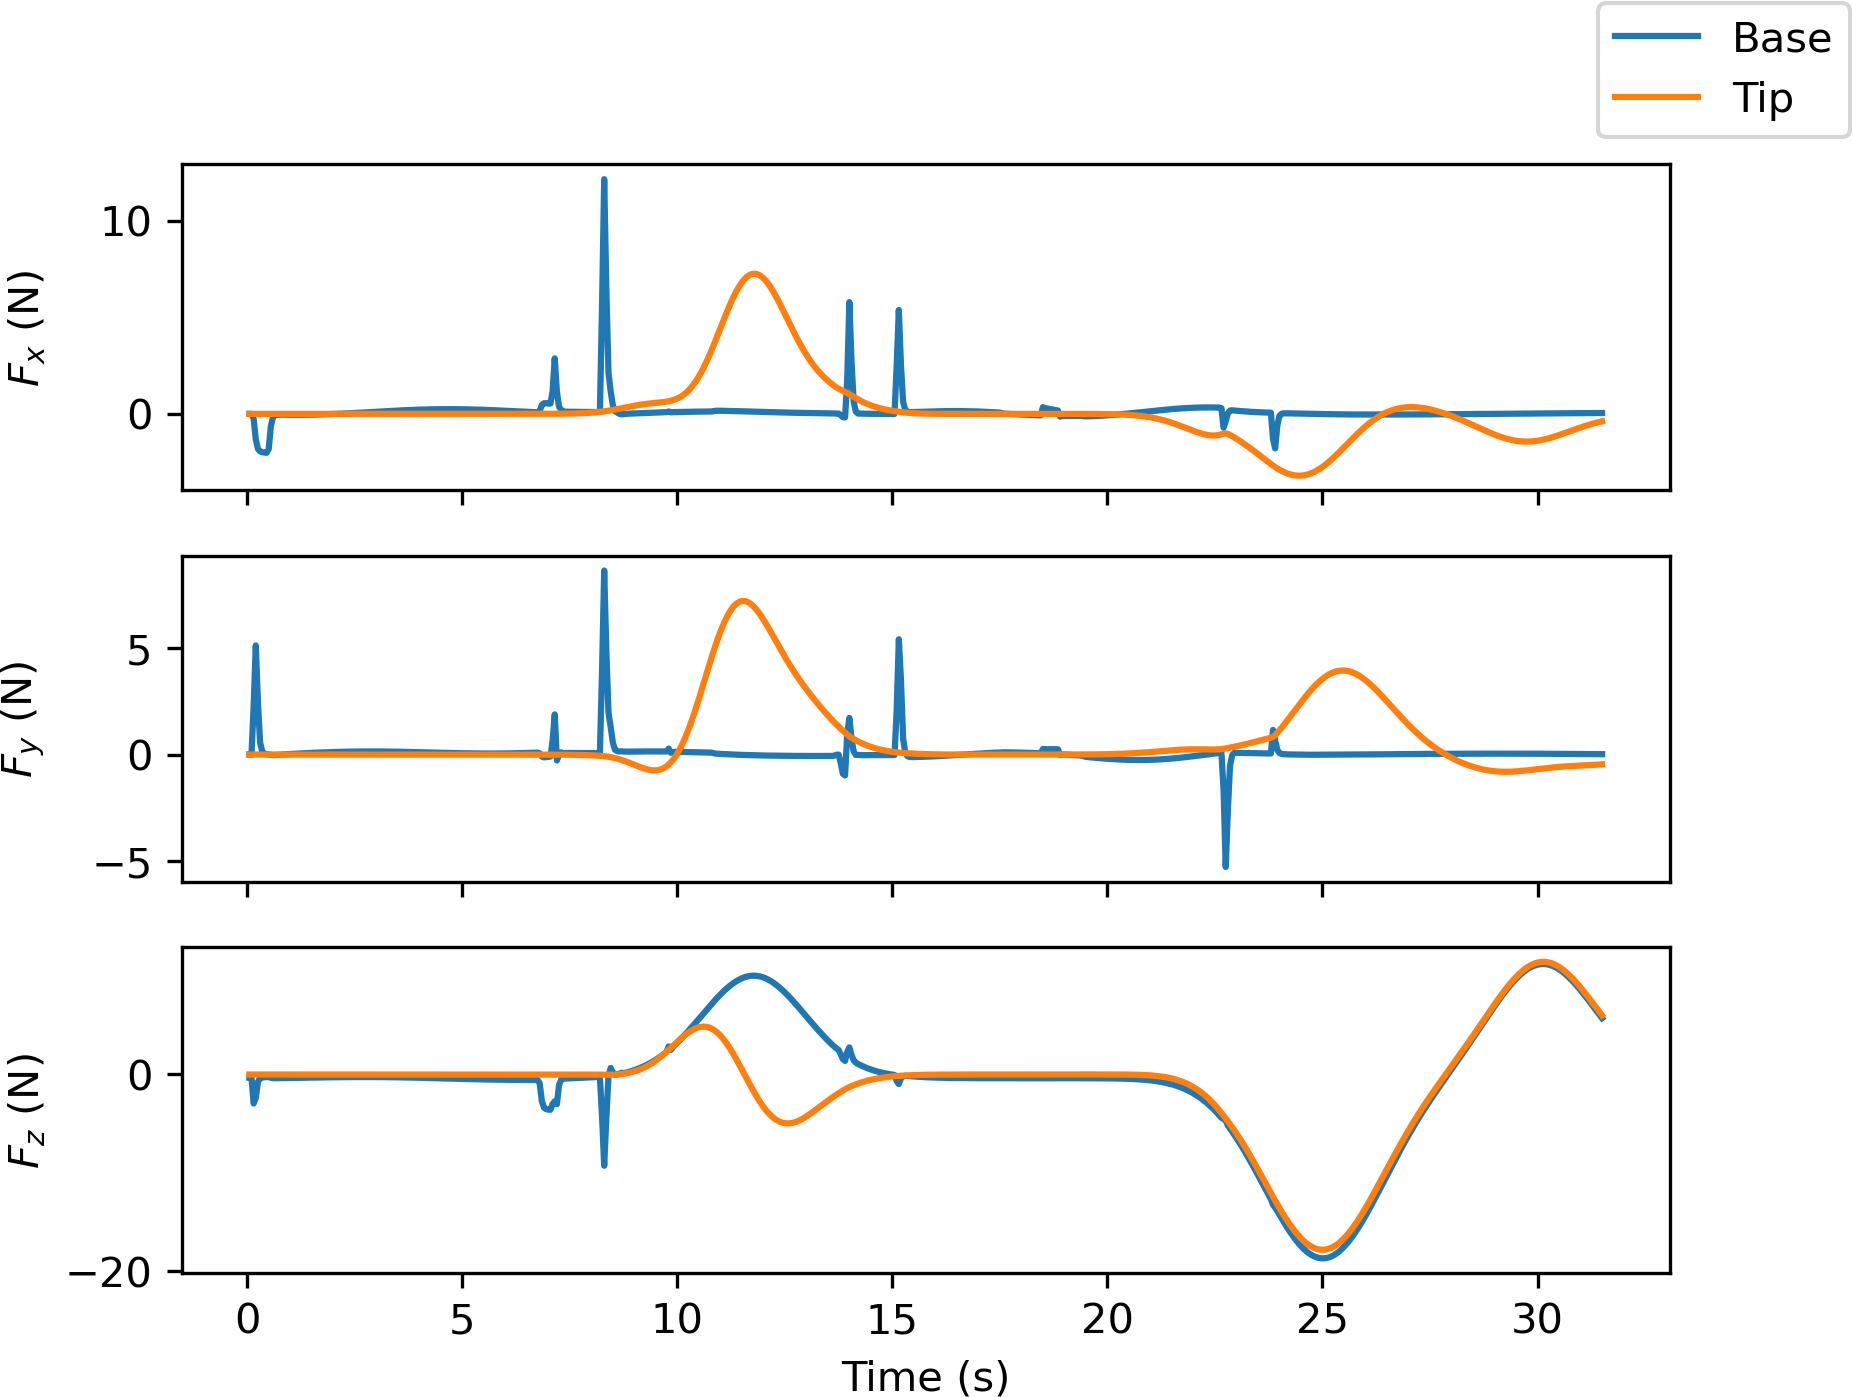
\includegraphics[width=0.55\textwidth]{slike/Fig03_24b.png}}
    \caption{Example of the running simulation}
    \label{fig:Coppelia}
\end{figure}

Another set of data was collected along with these data in simulation, with the same simulation-based setup except that no external forces were acting on the robot end-effector. The intention was to apply the approach introduced in \cite{Lutter2019} to learn the robot's inverse dynamics accurately, but it requires that no external forces are acting on the robot.

Following the data collection on the Franka robot in simulation, the data were also collected in the same setup using a real-world Franka robot to compare with the results obtained in simulation. The setup is shown in Figure \ref{fig:FrankaExp}. It features two force sensors: one was mounted under the robot base (Kistler 9257A sensor with Kistler 5070A charge amplifier and NI USB-6009 A/D converter for data acquisition)), and the other was mounted on the robot wrist (Hypersen FT-060 with built-in A/D converter and data acquisition over UDP), while the gripper was removed. Spatial calibration between the robot’s base and Kistler 9257A sensor (i.e., two coordinate frames in \cref{fig:FrankaExpSetup}) was achieved manually. The robot controller provided data about the robot state (joint positions, velocities and torques), while the forces (on base and wrist) force were measured directly using sensors.

Special consideration was given to interconnection between the robot base, Kistler force sensor underneath it and the environment to ensure the stability and repeatability of robot motion. This is more closely depicted in \cref{fig:FrankaBase}. The robot base was attached at four points defined by the manufacturer via bolts to the rigid aluminium sheet of 280x280x12 mm dimensions. This was then secured to the sensor top surface at predefined attachment points with sink-in head screws so that the robot lies flat on the aluminium plate. This was then attached to the aluminium sheet of 280x280x12 mm dimensions to provide extra stability when attaching it to the environment (e.g., floor). It should be noted that special care was given to robot pose positioning relative to the sensor surface underneath to place as large as possible robot base footprint over it and ensure that in the initial configuration, the whole system was balanced (i.e., even without the bolts and screws).

\begin{figure}
    \centering
    \subfloat[Franka robot during measurements with installed sensor under the base\label{fig:FrankaExpSetup}]{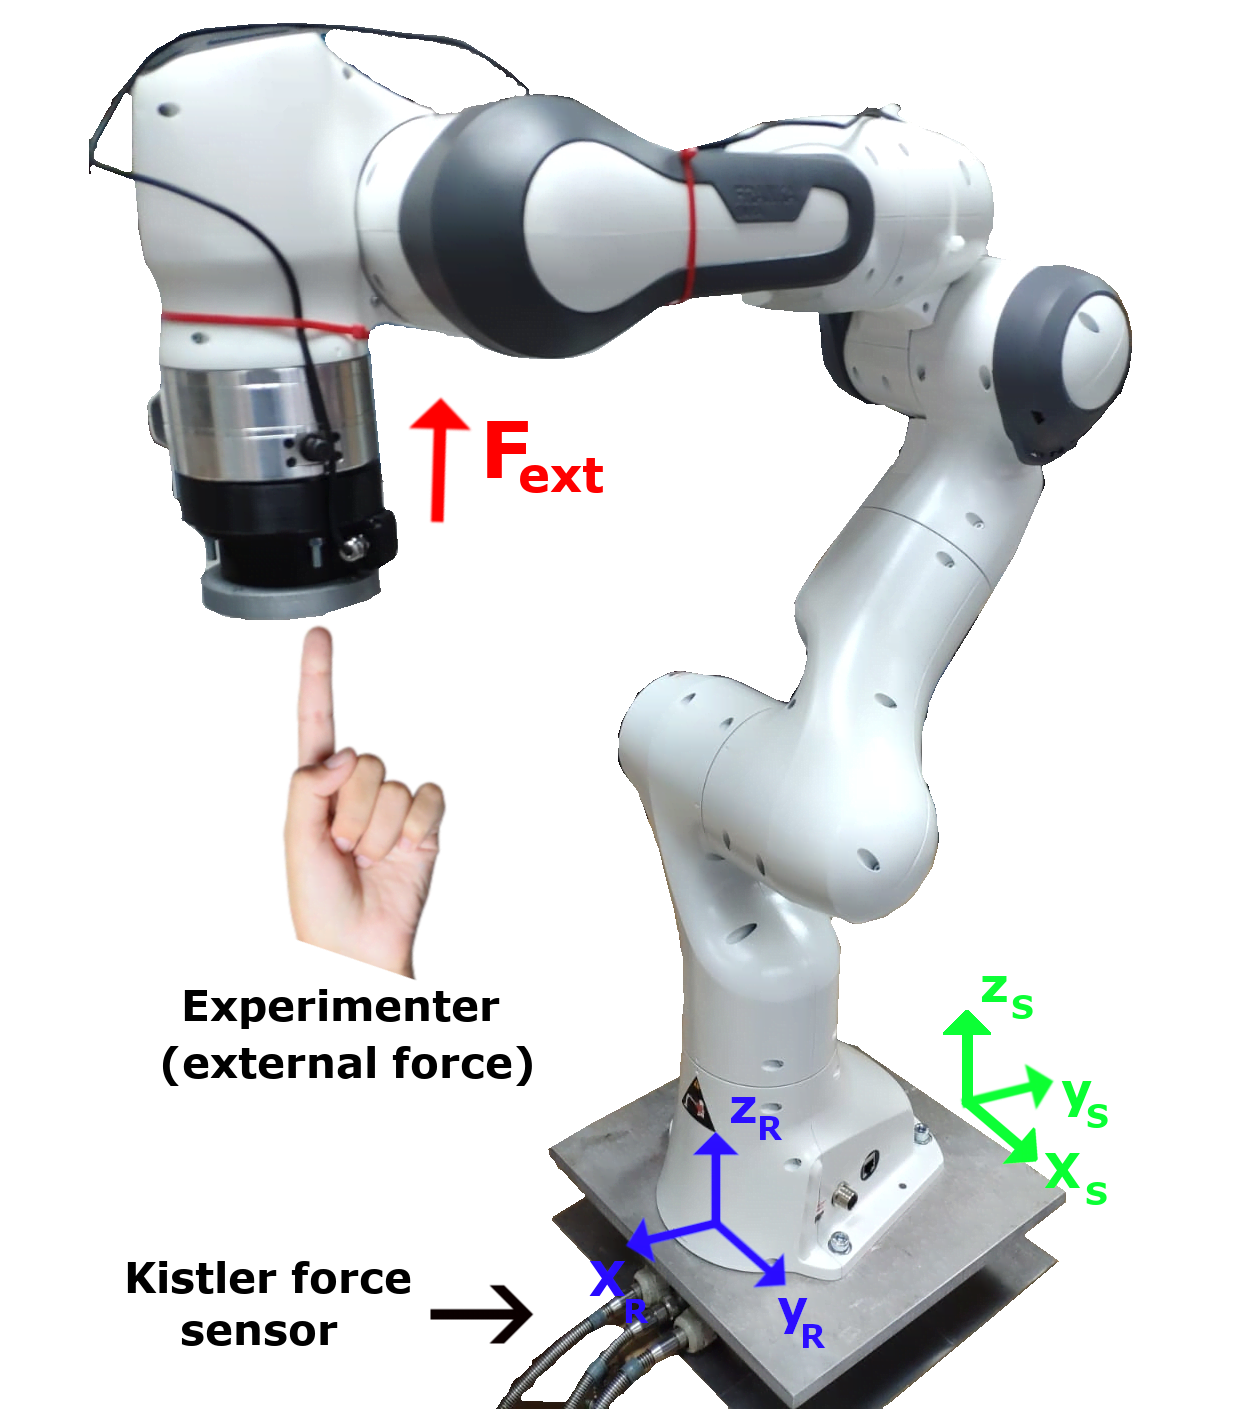
\includegraphics[width=0.45\textwidth]{slike/Fig03_25a.png}}
    \hfill
    \subfloat[Interconnection between the robot base, force sensor and the environment\label{fig:FrankaBase}]{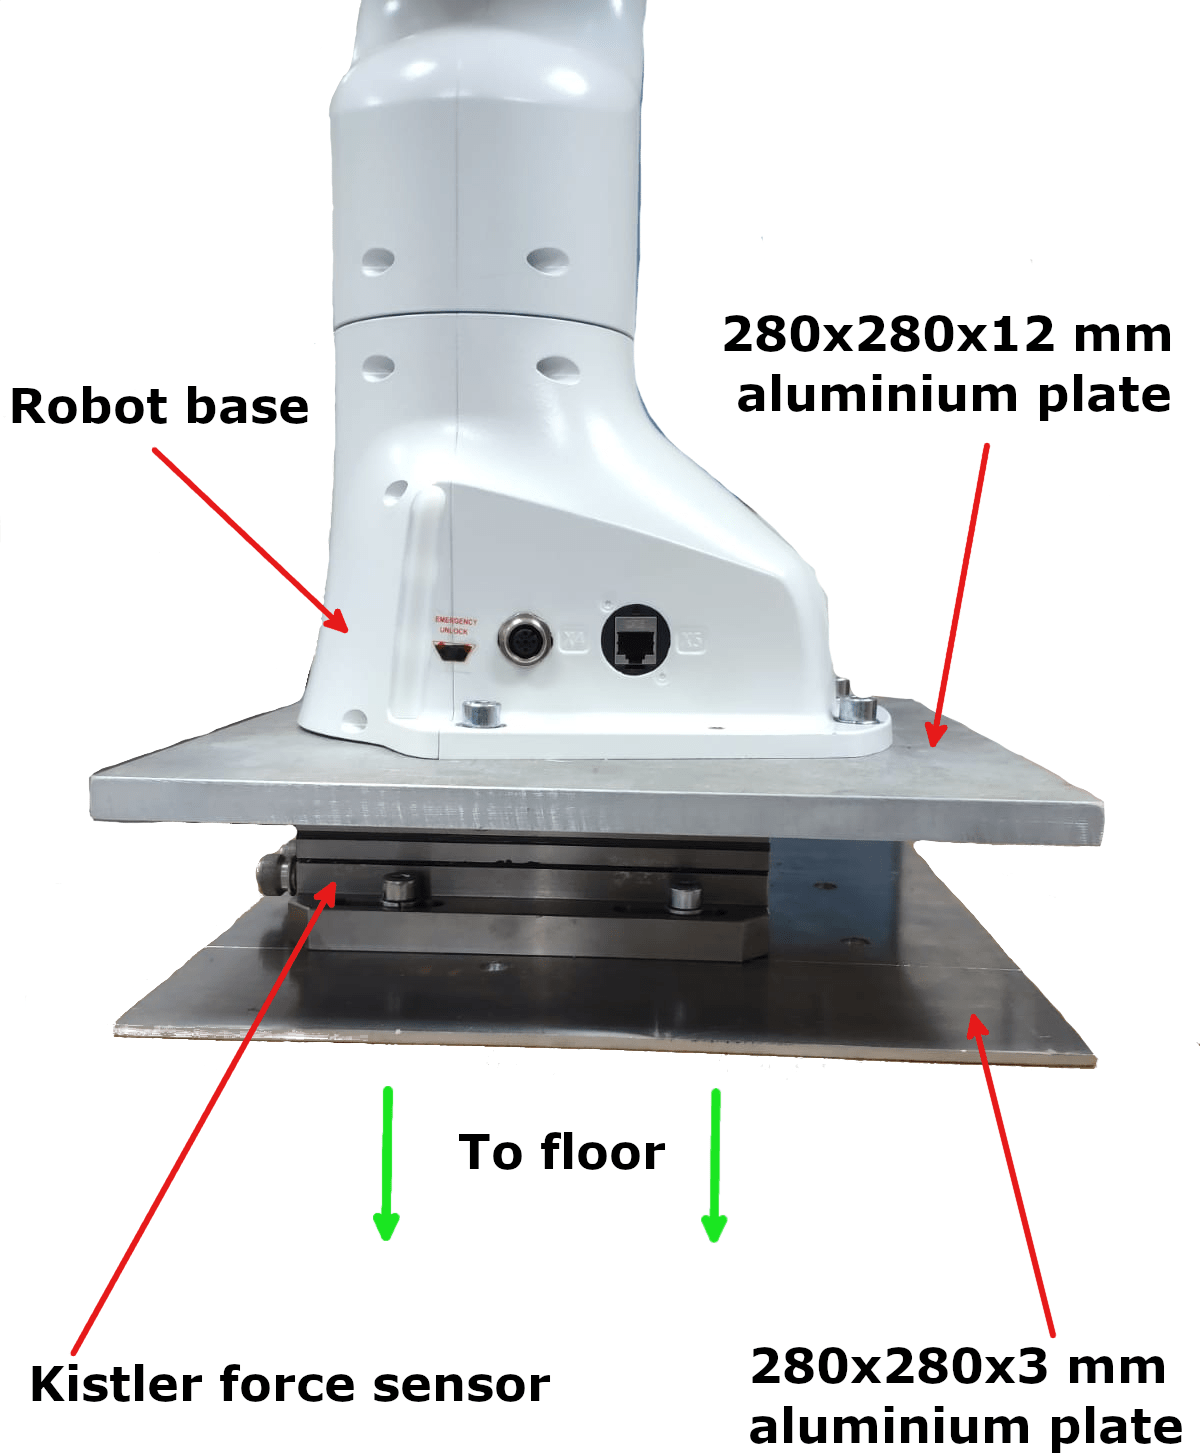
\includegraphics[width=0.45\textwidth]{slike/Fig03_25b.png}}
    \caption{Real-world experimental setup with Franka robot}
    \label{fig:FrankaExp}
\end{figure}

\subsection{Neural networks for end-effector force estimation}
\label{sec:MMNNEE}

Several neural networks of different types of architectures were trained with varying hyperparameters. The overview of the trained neural networks with their respective hyperparameters is summarised in Table \ref{tab:NetworksMover} using the data obtained on Mover 6 robot. The inputs to the network were the forces measured using the sensor mounted under the robot base, possibly with the inclusion of joint positions, as indicated in the table. The outputs were the forces measured using the sensor mounted on the interaction device. Please note that MLP networks have a higher number of neurons per layer than other architectures, which is based on previous experience in the field and on the fact that MLP does the learning on raw input data rather than temporal features (which is the case with convolutional and LSTM networks), and thus need more neurons to generalise appropriately. In convolutional and LSTM networks, a single 1D convolution or LSTM layer was used at the beginning of the network, reasoning that a single layer is enough for the data of relatively low dimensionality and complexity to extract temporal features. Therefore, the number of units in those layers was fixed to 8 for all training instances. 

\begin{table}
    \centering
    \caption{Trained neural networks for force estimation with selected hyperparameters for Mover6 robot}
    \label{tab:NetworksMover}
    \begin{tabular}{cccccc}
        \toprule
        \textbf{No.} & \textbf{Architecture} & \textbf{Joint pos.} & \textbf{FC Layers}\tablefootnote{Fully connected layers} & \textbf{Neurons} & \textbf{Seq. length}  \\
        \midrule
        1 & MLP & No & 3 & 64 & / \\ % mlp_01
        2 & MLP & Yes & 3 & 64 & / \\ % mlp_02
        3 & MLP & Yes & 2 & 32 & / \\ % mlp_03
        4 & Conv & No & 3 & 32 & 10 \\ % conv_01
        5 & Conv & Yes & 2 & 16 & 10\\ % conv_02
        6 & Conv & Yes & 2 & 16 & 5 \\ % conv_03
        7 & LSTM & No & 2 & 16 & 10 \\ % lstm_01
        8 & LSTM & Yes & 2 & 16 & 10 \\ % lstm_02
        9 & LSTM & Yes & 2 & 16 & 5\\ % lstm_03
        \bottomrule
    \end{tabular}
\end{table}

Similarly to Mover 6, neural networks were also trained with data obtained with the Franka robot and are summarised in Table \ref{tab:NetworksFranka}. The inputs to the network were the forces measured with the sensor mounted under the robot base, joint positions, velocities and accelerations, and possibly joint torques, as indicated in the table. As before, three types of architectures were used: multilayer perceptron, convolutional neural networks and LSTM networks. Neural network inputs on the Franka robot have higher dimensionality for all the architectures since more features are available (joint positions, velocities and accelerations, vs only joint positions with the Mover6 robot). With the increased complexity of input data, more neurons are needed in each layer to process such data and generalise properly.

Additionally, in convolutional and LSTM networks, a single layer extracted temporal features from sequential data. However, the number of units was higher than one used on the Mover6 robot, again due to the greater complexity of input data, explained earlier in this paragraph. Therefore, the number of units in those layers was kept at the value of 16 (vs 8 with the Mover6 robot). Then two fully connected layers followed at the end of the networks for all training instances (the latter is true also for MLP networks).

The expectation is that neural networks will capture Franka robot dynamics more accurately due to additional features provided as inputs when compared to Mover6 that provides fewer features to learn on.

Following these networks, two more networks were obtained using parameter optimisation to obtain more accurate estimates. The optimised hyperparameters were the number of LSTM layers, the number of LSTM units per layer, the number of fully connected layers, the number of units per layer, and the activation function. These networks are included in the table and are marked appropriately. Contrary to the others, they have two LSTM layers with 32 units each and use ReLU as an activation function. These networks are the best-performing ones selected during the optimisation process amongst those considered, with different values of hyperparameters.

\begin{table}
    \centering
    \caption{Trained neural networks for force estimation with selected hyperparameters for Franka robot}
    \label{tab:NetworksFranka}
    \begin{tabular}{cccccc}
        \toprule
        \textbf{No.} & \textbf{Architecture} & \textbf{Joint torques} & \textbf{FC Layers} & \textbf{Neurons} & \textbf{Seq. length}  \\
        \midrule
        1 & MLP & No & 2 & 32 & / \\ % mlp_01
        2 & MLP & Yes & 2 & 32 & / \\ % mlp_03
        3 & MLP & Yes & 2 & 16 & / \\ % mlp_04
        4 & Conv & No & 2 & 16 & 10 \\ % conv_01
        5 & Conv & No & 2 & 16 & 5\\ % conv_02
        6 & Conv & Yes & 2 & 16 & 5 \\ % conv_03
        7 & LSTM & No & 2 & 16 & 10 \\ % 
        8 & LSTM & Yes & 2 & 16 & 10 \\ % 
        9 & LSTM & Yes & 2 & 16 & 5\\ % 
        \midrule
        10 $^*$ & LSTM & No & 2 & 16 & 10\\
        11 $^\dagger$ & LSTM & Yes & 2 & 16, 48 & 10 \\
        \bottomrule
        \multicolumn{6}{l}{\footnotesize{$^*$ Optimised architecture: three LSTM layers with 56, 48 and 16 cells, respectively }}\\
        \multicolumn{6}{l}{\footnotesize{$^\dagger$ Optimised architecture: two LSTM layers with 64 and 56 cells, respectively}}
    \end{tabular}
\end{table}

% PROMJENA OD OPTIMIZACIJE
The goal of training different architectures of neural networks with different hyperparameters was not to identify the optimal hyperparameters or architecture. Instead, the main goal was to identify what architecture is best-suited for the problem at hand and whether the inclusion of additional information provided by the robot as inputs (in our case, joint torques) significantly affects the performance of the neural networks.

Thus, only a relatively small-scale hyperparameter optimisation was conducted to assess if there was some improvement in network performance. Therefore, after training the networks from \cref{tab:NetworksFranka}, the hyperparameter optimisation was performed. However, please note that optimisation was only performed for LSTM architecture, since it was identified as the best-performing one, which is shown later on in \cref{sec:ResultsEE}. Hyperparameters that were optimised were: activation function, number of LSTM layers and number of cells per each layer, number of dense layers and number of neurons per each layer. The hyperparameters search space was thus summarised in \cref{tab:HPSearchSpace}.

\begin{table}
    \centering
    \caption{Hyperparameters search space}
    \label{tab:HPSearchSpace}
    \begin{tabular}{ll}
        \toprule
        \textbf{Hyperparameter} & \textbf{Possible values}\\
        \midrule
        Activation function & ReLU, ELU, Tanh \\
        Number of LSTM layers & 1 -- 3 \\ % mlp_03
        Number of cells per LSTM layer & 8 -- 64, step 8 \\ % mlp_04
        Number of FC layers & 2 -- 4 \\ % conv_01
        Number of neurons per FC layer & 8 -- 64, step 8 \\ % conv_02
        \bottomrule
    \end{tabular}
\end{table}

The results of hyperparameter optimisation is given and discussed in \cref{sec:ResultsEE}.

\subsection{Neural networks for joint torques estimation}

Following the training of neural networks for end-effector force estimation for the Franka robot, another experiment was conducted to assess the performance of the robot inverse dynamic model approximated by various neural networks and to compare it with the analytical inverse dynamic model identified in \cite{Gaz2019}, and DeLaN network \cite{Lutter2019}. The inverse dynamic model presented here is also based on neural networks, which take joint positions, velocities and accelerations and output control torques.

The inverse dynamic model is derived from the Euler-Lagrange equation as
\[
    \vtau=\mH(\vq)\ddot{\vq}+\vc(\vq,\dot{\vq})+\vg(\vq)+\vtau_f(\dot{\vq})
    \label{eq:InvDyn}
\]
where $\mH$ is the mass matrix, $\vc$ is a term describing torques due to centripetal and Coriolis forces, $\vg$ is the gravity term, $\vtau_f$ is the torque due to friction, and $\vtau$ is the vector of joint-side torques. These quantities are dependent on either joint positions $\vq$ or joint velocities $\dot{\vq}$ (or both), and all these data are available in the simulation datasets. This experiment differed from the previous in that the neural network outputs were joint torques (internal measurements provided by the robot controller) instead of end-effector forces.

For this experiment, neural networks were trained with simulation data and with real-world data. Please note that in this experiment, the force sensor was mounted under the robot base between two aluminium plates, as before, and shown in \cref{fig:FrankaTorqueSetup}. However, although the experimental setup for this experiment is similar to the previous one (same robot, same sensor under the robot base), the difference is that this time no force sensor was mounted at the robot's tip.

\begin{figure}
    \centering
    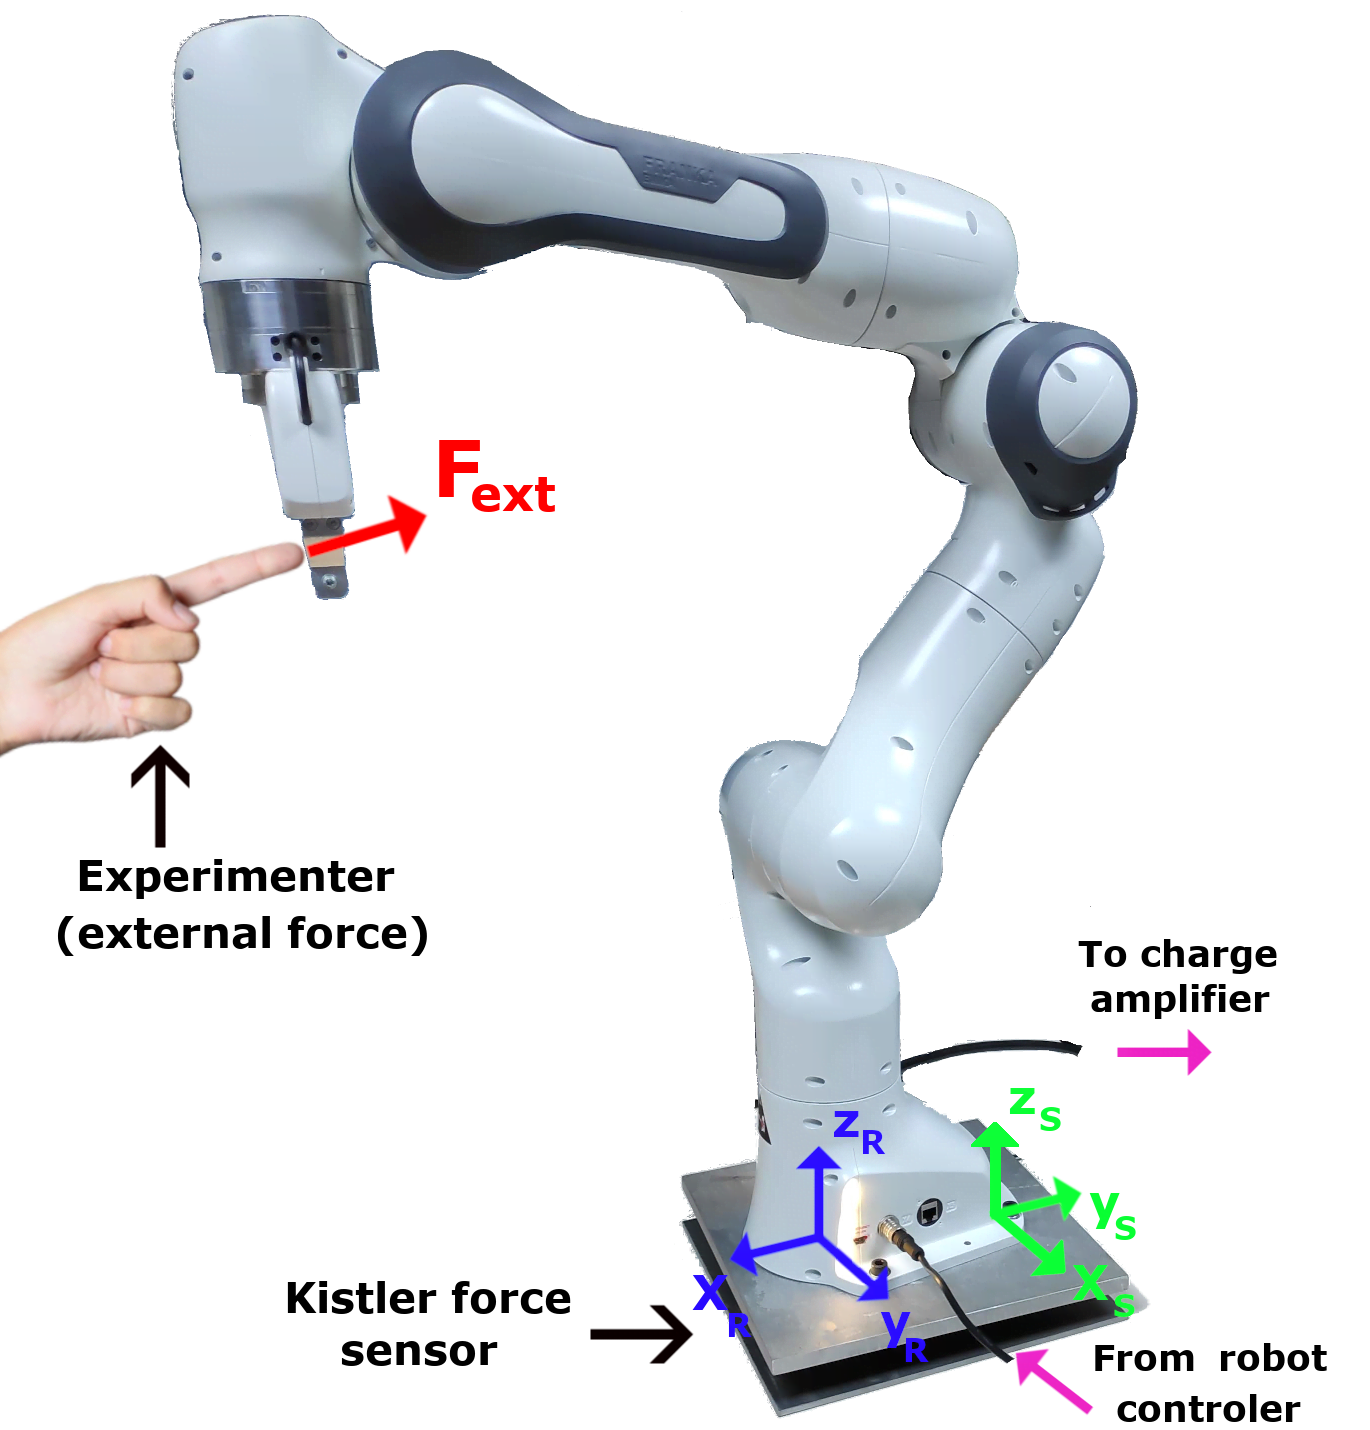
\includegraphics[width=0.5\textwidth]{slike/Fig03_26.png}
    \caption{Real Franka robot experimental setup for joint torques estimation}
    \label{fig:FrankaTorqueSetup}
\end{figure}

Architectures of trained networks for joint torques estimation are shown in \cref{tab:NetworksFrankaTorque}. Please note that only a single instance of each architecture is trained per dataset. The results are reported and discussed in \cref{sec:ResJoint}.

\begin{table}
    \centering
    \caption{Trained neural networks for joint torques estimation}
    \label{tab:NetworksFrankaTorque}
    \begin{tabular}{cccc}
        \toprule
        \textbf{No.} & \textbf{Architecture} & \textbf{Dataset} & \textbf{External forces} \\
        \midrule
        1 & DeLaN & Simulation & No \\ % lnn_prazni_02
        2 & DeLaN & Simulation & Yes \\ % lnn_teret_02
        3 & MLP & Simulation & Yes \\ % mlp_tau_01
        4 & Conv & Simulation & Yes\\ % conv_teret_torque_01
        5 & LSTM & Simulation & Yes \\ % lstm_teret_torque_01
        \midrule
        6 & DeLaN & Real world & Yes \\ % lnn_franka_01
        7 & MLP & Real world & Yes\\% mlp_franka_torque_01
        8 & Conv & Real world & Yes\\ % conv_franka_torque_01
        9 & LSTM & Real world & Yes\\ % lstm_franka_torque_01
        \bottomrule
    \end{tabular}
\end{table}

Please note that this experiment could not be conducted on the Mover6 robot since the robot's controller does not provide joint torques, which are used as network outputs in this approach.

% NOVO OPTIMIZACIJA
Finally, and similarly to the previous experiment, a hyperparameter optimisation procedure was performed to assess if there was some improvement in the performance of the networks. The search space was the same as one in \cref{sec:MMNNEE}, while the results are presented and discussed in \cref{sec:ResJoint}.
% NOVO KRAJ

As a final experiment on joint torques estimation, the base-mount force sensor was replaced by four single-axis force sensors. These low-cost sensors were based on strain gauges and are shown in \cref{fig:StrainGauge}. They were put into a rectangular configuration shown in \cref{fig:Platform}, on top of which an aluminium plate with a robot mounted on it was put. This experiment was conducted only using a real-world Franka robot since these sensors are not available in the simulation. Data acquisition was based on an HX711 24-bit A/D converter and Arduino Uno (the same Arduino board was used to acquire data from all the sensors).

The procedure of collecting data was the same as in previous experiments, where the experimenter applied the force to the robot end-effector (\cref{fig:FrankaTorqueSetup}). However, please note that in this experiment, the dataset was not as extensive and as diverse as in the previous since the goal was to assess the possibility of using multiple low-cost and simple sensors to achieve comparable performance to one using a 3-axis force sensor (which was used in previous experiments).

\begin{figure}
    \centering
    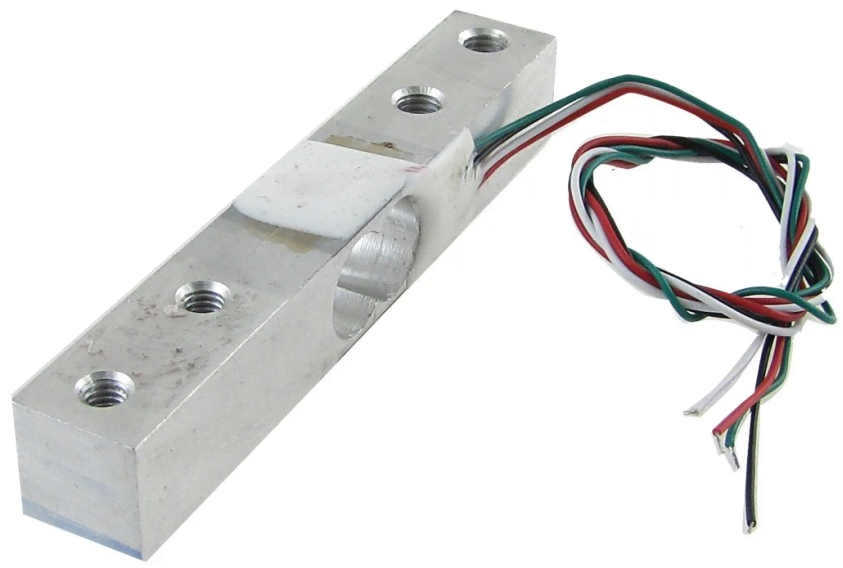
\includegraphics[width=0.5\textwidth]{slike/Fig03_27.png}
    \caption{Low-cost single-axis force sensor}
    \label{fig:StrainGauge}
\end{figure}

The network architectures trained were multilayer perceptron, convolutional, and LSTM networks (one of each, as in the previous experiment).

\begin{figure}
    \centering
    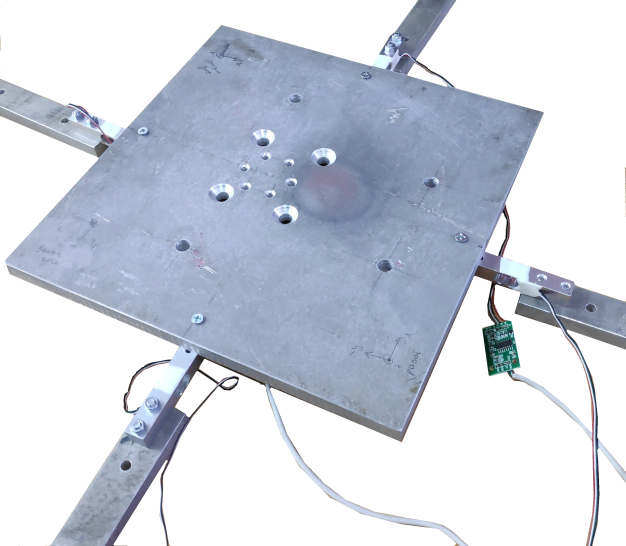
\includegraphics[width=0.6\textwidth]{slike/Fig03_28.png}
    \caption{Base force measurement platform based on multiple single-axis force sensors}
    \label{fig:Platform}
\end{figure}

\newpage
\chapter{RESULTS AND DISCUSSIONS}
\label{chap:Results}

\section{Neural network-based obstacle avoidance for mobile robots}

The results obtained in the experiments show that the neural networks for obstacle avoidance trained entirely with the data obtained in simulation can have good performance in the real world without any additional training with real-world data. In the following subsections, each of the experiment results is reported and discussed.

\subsection{Parameters identification experiment}\label{Sec:ResLabelling}

The first thing to notice in this experiment is that, by using datasets created by using different parameters for the number of LiDAR points and thresholds, the ratio between numbers of positive and negative training samples is different, although the same raw data are used. That is because, when using lower threshold values, the robot can come closer to the obstacle and for that reason, there are more positive samples than higher threshold values. Similar reasoning can be applied to the other parameter in question, the number of points needed to classify a sample as negative. Note that positive samples likely won't result in a crash, while negative samples would result in a collision. This parameter also had a significant impact on the imbalance between the positive and negative samples in the dataset since the number of points is a crucial parameter to decide if something is an obstacle or not. The ratios between positive and negative samples as a function of these parameters are shown in \cref{fig:Brojevi}. Finally, please note that data in the figure is for the neural network for moving forward; similar trends emerge for neural networks for going left and right.

\begin{figure}
\centering
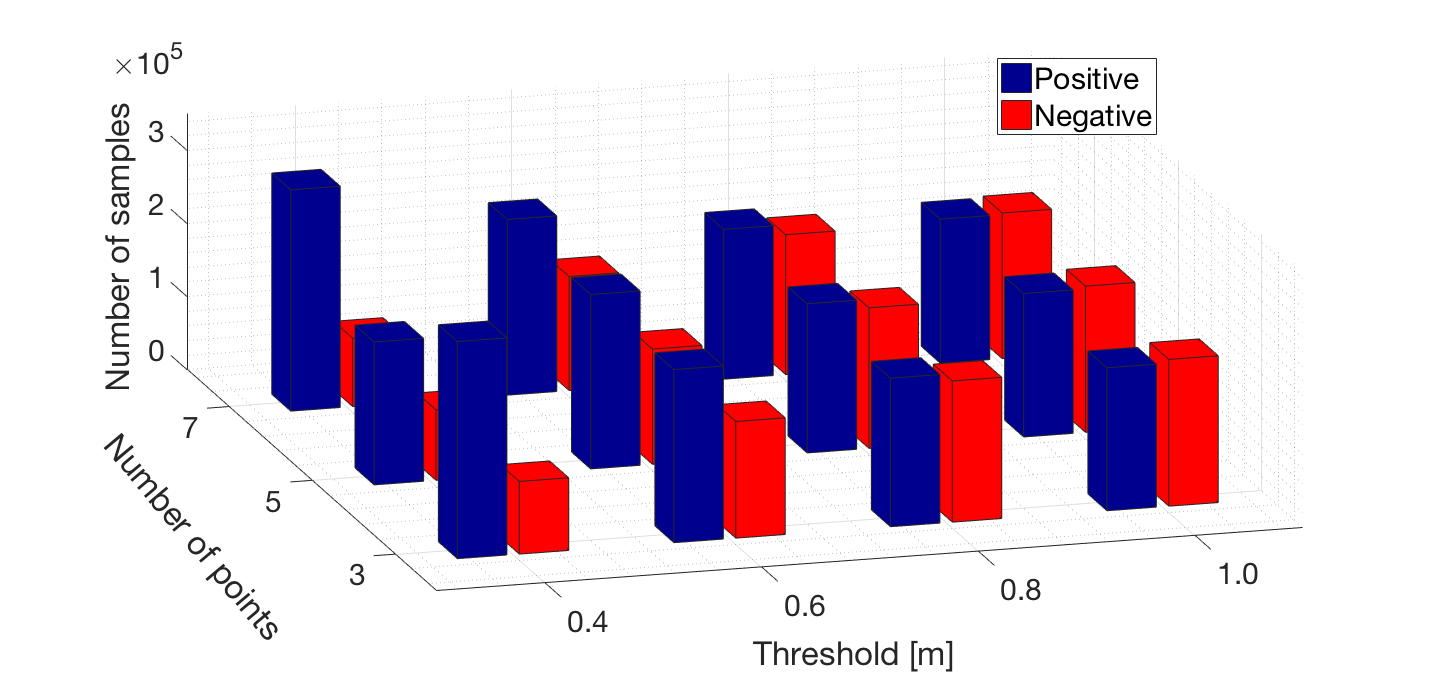
\includegraphics[width=0.9\textwidth]{slike/brojevi}
\caption{The number of positive and negative samples per dataset}
\label{fig:Brojevi}
\end{figure}

It was also observed that there were more crash events for datasets created with threshold parameter values of 0.4 m and 0.6 m than with other setups. It is likely due to the uneven numbers of positive and negative samples used for the training of neural networks (as per Figure \ref{fig:Brojevi}). These datasets have a significantly higher number of positive samples than negative, which is not the case with setups with threshold parameters equal to 0.8 m and 1 m. This disbalance emphasises the importance of negative samples for learning and is in line with \cite{Gandhi2017}, and neural networks may need to be fed with more training samples given the current ratio between negative and positive samples to achieve improved performance. The experiment also demonstrated that for neural networks trained with a threshold of  1 m robot executed a significant number of in-place rotations due to the course's narrowness (which was 2.16 m and augmented with additional obstacles). The robot is 0.35 m in diameter, so it needed additional in-place rotations to ``find'' an obstacle-free route.

Out of 60 trials with different neural networks (i.e., neural networks trained with different datasets), in 47 trials, the robot did not complete the course (i.e., get to the other side of the corridor/course), while in the other 13 trials the course was completed. This outcome is not surprising since the robot is not aware of the goal point. It freely roams through the course, going forward when the space in front of it is obstacle-free, and avoiding the obstacle otherwise, which often results in the robot turning away from the course end (which should not be considered as a flaw of the approach, but the limitation of the experimental setup).

\begin{table}[H]
\centering
\caption{The summary of parameter identification experiment results with numbers of completed courses, crash events, loops and local minima per each combination of parameters used.}
\label{Tbl:Stats}
\begin{tabular}{ccccccc}
\toprule
\textbf{Points} & \textbf{Threshold} & \textbf{Completed} & \textbf{Crashes\tablefootnote{Total number of crashes}} & \textbf{Thin obs.\tablefootnote{Number of crashes into thin obstacle near course end}} & \textbf{Loop} & \textbf{Local minimum}\\
\midrule
\multirow{4}{*}{3} & 0.4 m & 0 & 5 & 1 & 0 & 0\\
& 0.6 m & 1 & 2 & 1 & 2 & 0\\
& 0.8 m & 0 & 0 & 0 & 5 & 0\\
& 1.0 m & 0 & 2 & 2 & 0 & 3\\
\midrule
\multirow{4}{*}{5} & 0.4 m & 0 & 4 & 0 & 1 & 0\\
& 0.6 m & 1 & 3 & 0 & 1 & 0\\
& 0.8 m & 4 & 1 & 1 & 0 & 0\\
& 1.0 m & 4 & 1 & 1 & 0 & 0\\
\midrule
\multirow{4}{*}{7} & 0.4 m & 1 & 4 & 1 & 0 & 0\\
& 0.6 m & 0 & 4 & 3 & 1 & 0\\
& 0.8 m & 2 & 3 & 3 & 0 & 0\\
& 1.0 m & 0 & 1 & 1 & 0 & 4\\
\bottomrule
\end{tabular}
\end{table}

Table \ref{Tbl:Stats} shows a summary of the conducted experiments. From it, it is evident that setups with 7 LiDAR points needed to classify a sample as negative perform worse than other setups when encountering obstacles with a thin profile, like one right before the course end, as shown in Figure \ref{Fig:LabellingTraj}.
The robot collided with that obstacle significantly more often using this setup than with other setups (eight times vs six times using all other setups combined). Such outcomes are most likely because it does not classify such an obstacle as a negative sample. After all, it usually does not occupy at least 7 points in the LiDAR scan. In addition, it is worth noting that the robot avoided that obstacle several times, so it may be concluded that the angle of approach to it may be critical to its avoidance since when approaching it at different angles results in a different number of LiDAR scan points representing that obstacle, as Figure \ref{Fig:Tocke} demonstrates. Given that, when the robot approaches that obstacle frontally, it ``sees'' only 4 LiDAR points, for the approach at 15$^{\circ}$ 8 points, at 30$^{\circ}$ 10 points and 45$^{\circ}$ 12 points.

\begin{figure}
\centering
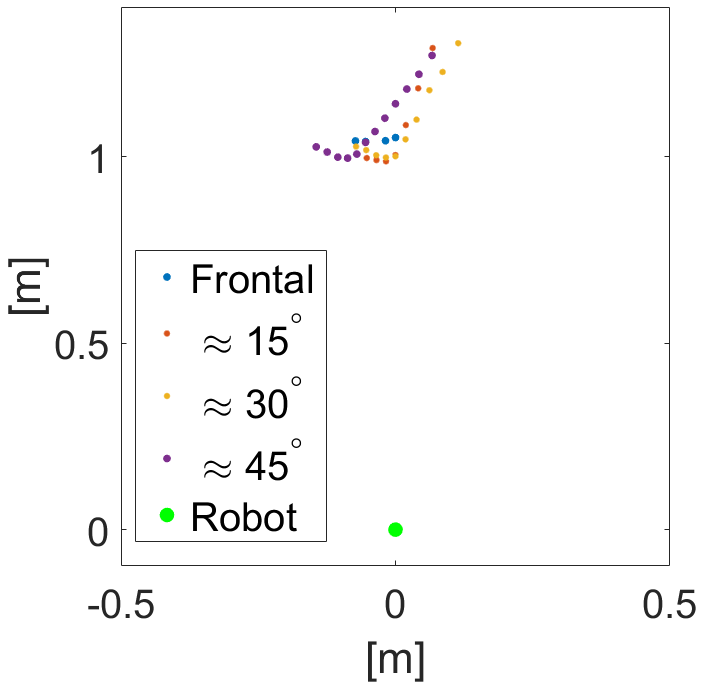
\includegraphics[width=0.5\textwidth]{slike/lidar_tocke.png}
\caption{Visualisations of LiDAR scan points when robot approaches thin obstacle from various angles}
\label{Fig:Tocke}
\end{figure}

The timings of experiment trials were recorded and reported for completed course trials, although completion times were not considered a performance metric. The average time and standard deviations per number of points are provided in \cref{Fig:Vrimena}, which demonstrate that the setup with three scan points performs better than others, likely because it can identify more obstacles than other setups and act accordingly, and more identified obstacles might also be a reason why the number of completed courses is so low with that setup compared to others. The setup with seven scan points performs slightly better than the one with five scan points. However, the course was completed only three times, compared to the setup with five scan points completed nine times. Thus, it needs additional testing trials to obtain more general results and draw definite conclusions (based on statistical testing).

\begin{figure}
\centering
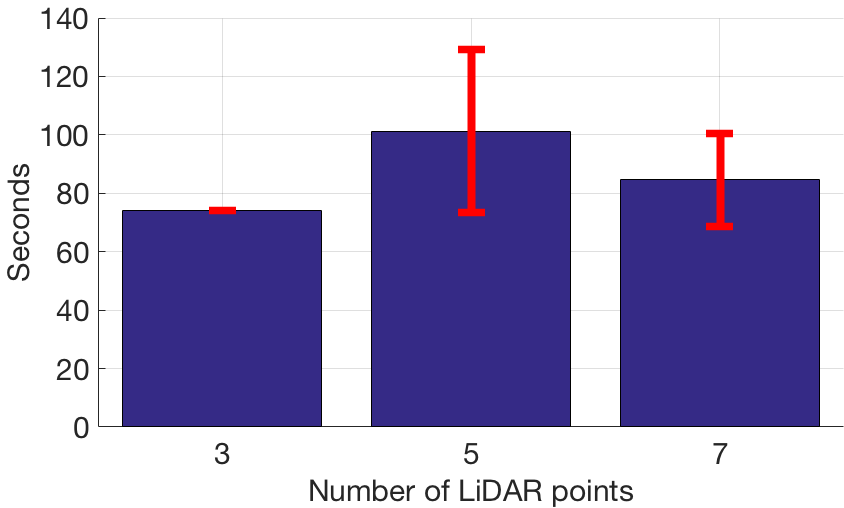
\includegraphics[width=0.5\textwidth]{slike/vrimena}
\caption{Time analysis of completed course trials}
\label{Fig:Vrimena}
\end{figure}

In some trials, the robot got stuck at local minima. It is noticeable that it only happened with setups that avoid obstacles at a 1 m threshold. Such an outcome is likely due to the narrowness of the experimental course because, at some points in the course, it is impossible to go forward given the sensor readings, so the robot keeps executing in-place rotation to the left and right interchangeably. This issue was resolved in the experiments that followed so that the robot applied a small forward velocity to break out the deadlock.

Results also demonstrated that setups that need 3 LiDAR points (or to some extent also 5 LiDAR points) to classify a sample as negative were too sensitive when using lower threshold values (0.4 m and 0.6 m), since the robot crashed into other obstacles (besides a thin obstacle near the course end) more often than other setups. The crashes might as well be due to the significantly higher number of positive samples than negative samples for training the neural networks for obstacle avoidance.

Examples of the robot trajectories obtained during the experiment are shown in Figure \ref{Fig:LabellingTraj}. Note that the trajectories were captured using AMCL \cite{Fox1997,Thrun2006} which introduces some additional positioning errors. Thus, sometimes in the image, it may seem that there is no crash (when there is, as in Figure \ref{Fig:LabellingTrajb}) or vice versa, that the robot passes ``through'' obstacle (when it passes very close to the obstacle, as in Figure \ref{Fig:LabellingTrajc}).

\begin{figure}
\centering
\subfloat[The trajectory of the completed course \label{Fig:LabellingTraja}]{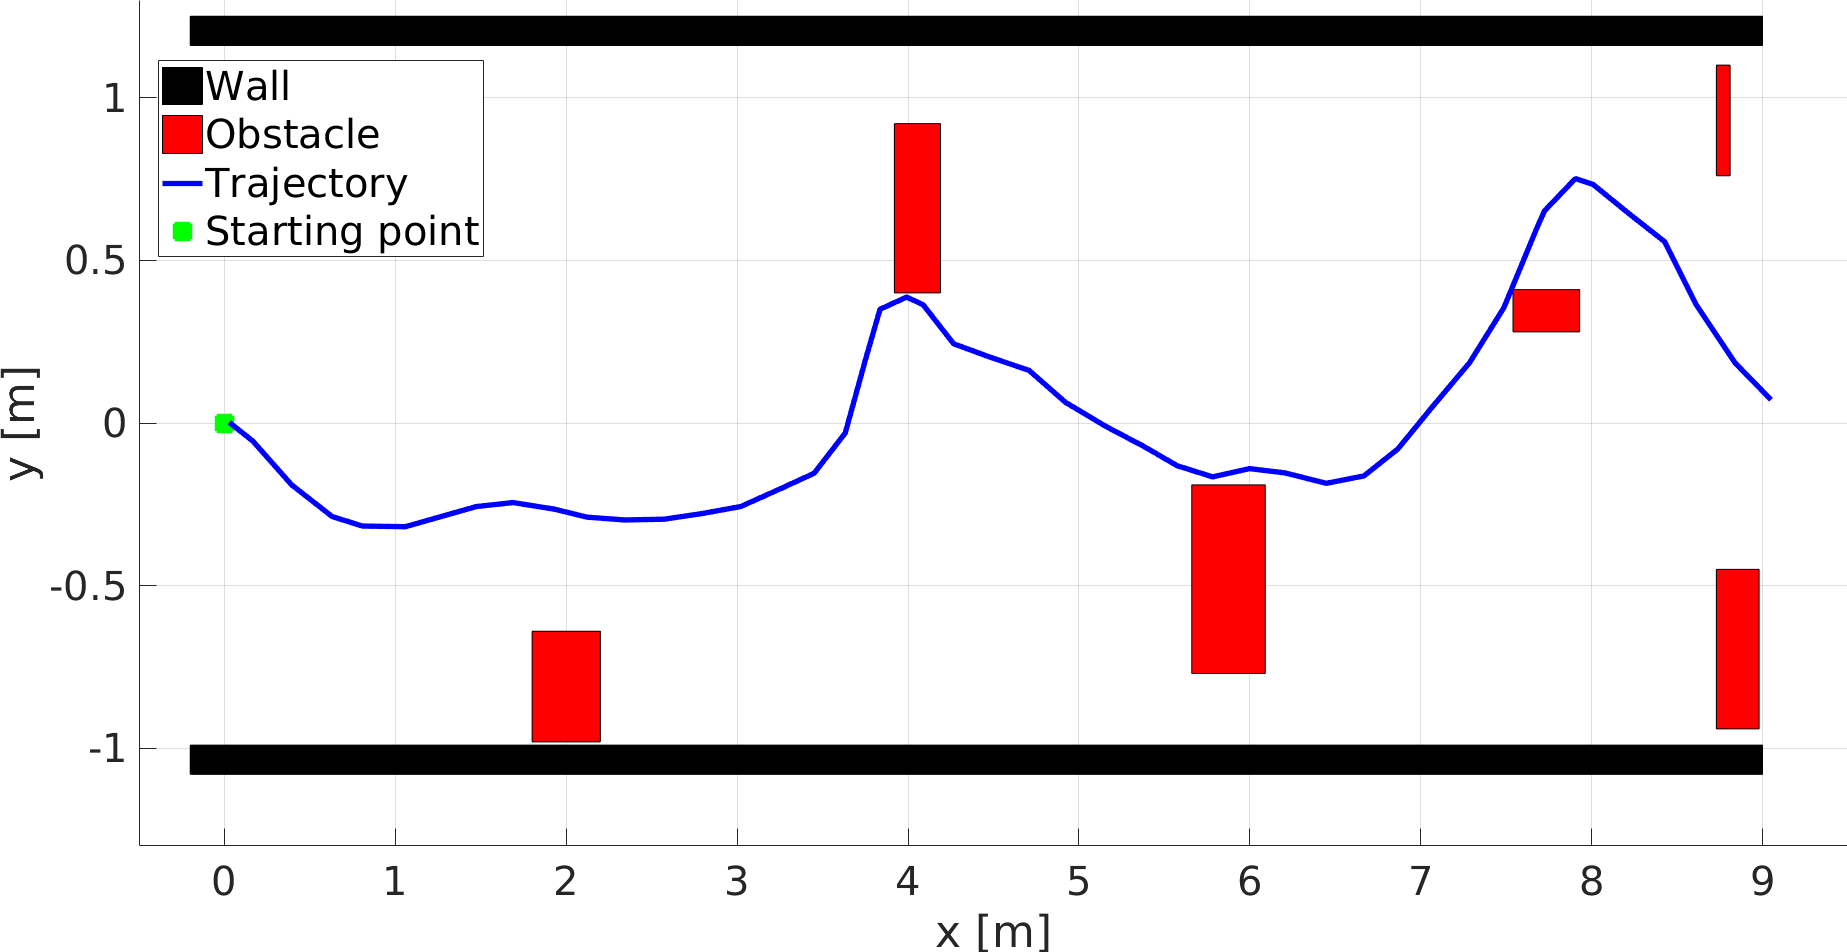
\includegraphics[width=0.495\textwidth]{slike/trajektorija_ok}}
\hfill
\subfloat[The trajectory of a course that resulted in a crash\label{Fig:LabellingTrajb}]{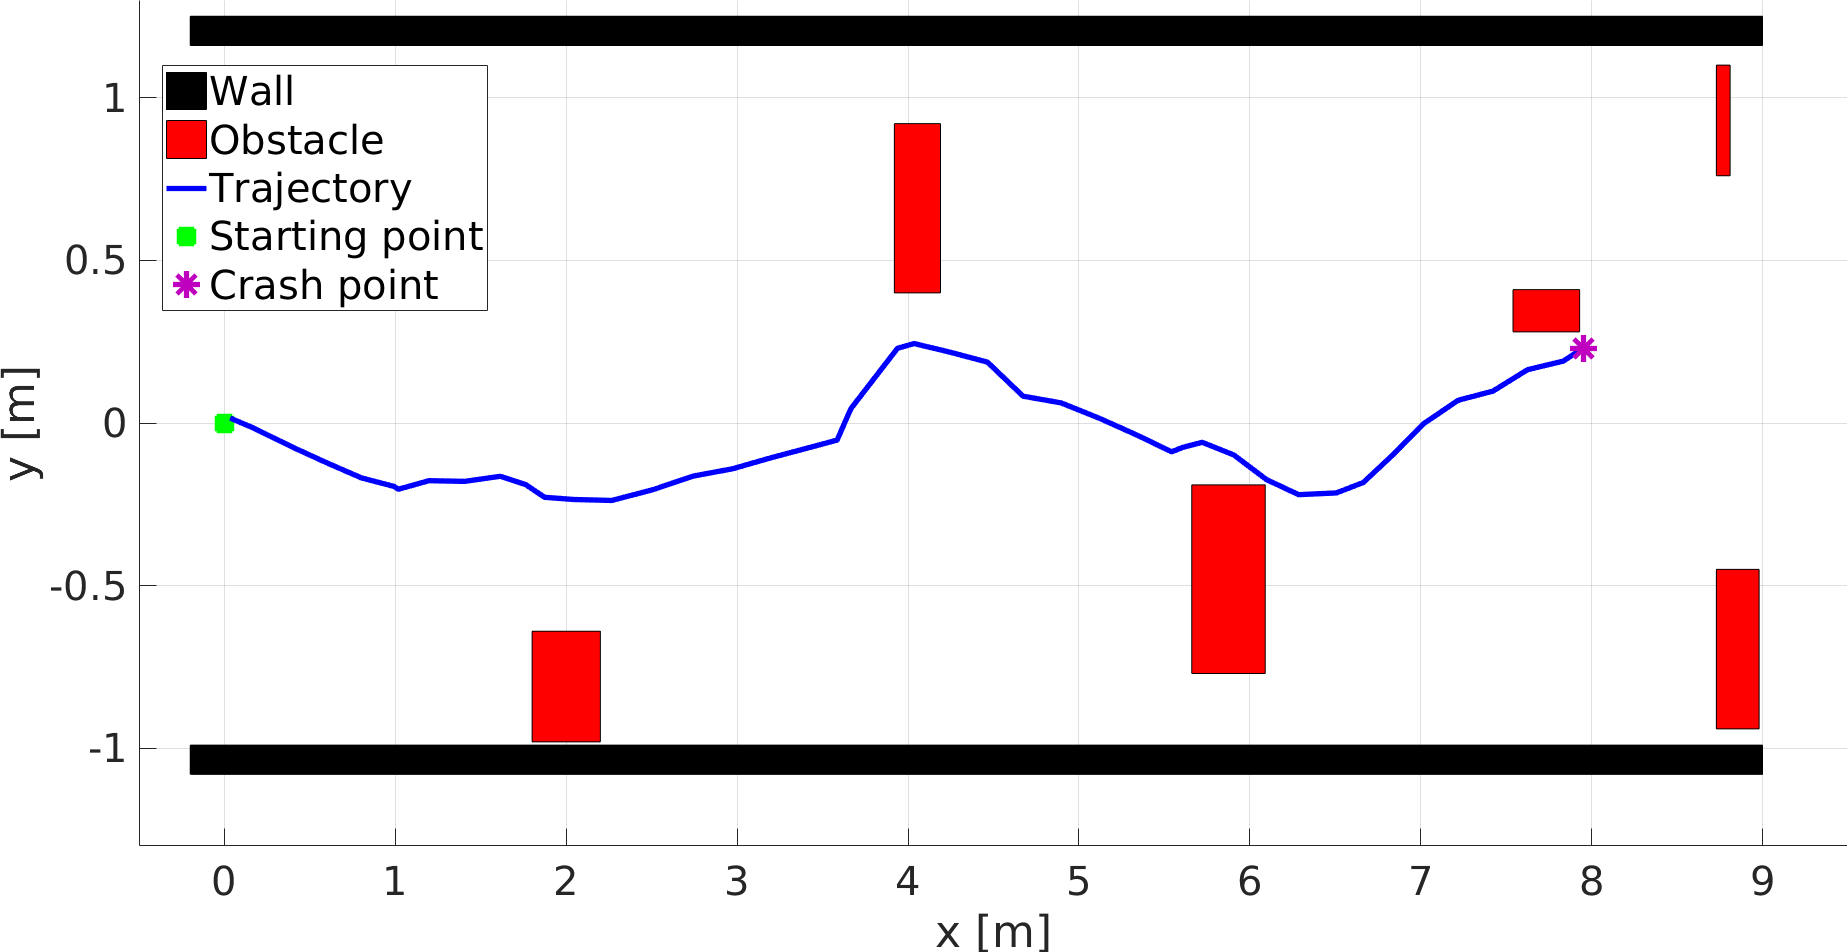
\includegraphics[width=0.495\textwidth]{slike/trajektorija_crash}}
\vfill
\subfloat[The trajectory of a course that resulted in a loop \label{Fig:LabellingTrajc}]{\includegraphics[width=0.495\textwidth]{slike/trajektorija_loop}}
\hfill
\subfloat[The trajectory of a course in which the robot got stuck at local minimum \label{Fig:LabellingTrajd}]{\includegraphics[width=0.495\textwidth]{slike/trajektorija_min}}

\caption{Examples of robot trajectories during the arameters identification experiment}
\label{Fig:LabellingTraj}
\end{figure}

Based on the obtained results in the experiment, it was decided to use datasets labelled with a threshold of 1 m and 5 LiDAR scan points for the experiments that followed, both in simulation (\cref{sec:SimulationRes}) and in the real world (\cref{sec:RealRes}).

\subsection{Simulation experiments}
\label{sec:SimulationRes}

In all 20 test runs of the first experiment in simulation, the run was terminated after 10 minutes without a crash. That summed up to a total of 200 minutes of driving without a crash in an environment cluttered with obstacles. These results demonstrated appropriate behaviour in simulation, which motivated us to further test the approach on the real robot. Examples of trajectories obtained during testing in the simulation are shown in Figure \ref{fig:Fig06}. However, it should be noted that if a more dense obstacle configuration was used, crashes might have occurred, but we believe that the used obstacle configuration (remember the size of the whole perimeter is 12.5 m $\times$ 12.5 m) is a good representation of a general office-type environment.

\begin{figure}
    \centering
    \subfloat{\includegraphics[width=0.495\textwidth]{slike/turkish/Fig06a.pdf}}
    \hfill
    \subfloat{\includegraphics[width=0.495\textwidth]{slike/turkish/Fig06b.pdf}}
    \caption{Example trajectories obtained while testing the proposed obstacle avoidance method in simulation.}
    \label{fig:Fig06}
\end{figure}

In the other simulation experiment, which contained a single moving obstacle in a small area, it was observed that the robot had no problem avoiding the moving obstacle if the obstacle velocity was small (0.1 m/s and 0.2 m/s, roughly less than robot velocity). However, crashes occurred with higher obstacle velocities (6 crashes with 0.4 m/s obstacle velocity, and with 0.8 m/s obstacle velocity, the robot could not get past the moving obstacle at any time). While interpreting these results, please keep in mind that the robot velocity was constant (0.2 m/s) and that neural networks controlling the robot were trained without moving obstacles in the scene, and that possibly improved performance could be achieved if moving obstacles are appropriately included in the training set. 

\subsection{Real-world experiments}
\label{sec:RealRes}

In real-world experiments, the first thing that was assessed was the computational speed of the proposed algorithm (mean values for 500 LiDAR scan cycles are reported; of note is that the median values were smaller than the average values in all cases). Each neural network (right, left, forward) took 0.773 ms to produce an output, while the preprocessing of raw LiDAR data (mainly separation to appropriate parts and formatting) took another 0.144 ms. The postprocessing (generation of velocity commands for the mobile robot) took an additional 0.237 ms. Thus, on average, the algorithm took 1.554 ms to produce a velocity command to the robot based on its input. This computational speed was more than enough in our case since LiDAR maximum rotation frequency was about 7 Hz (i.e., it took about 142 ms to make a single rotation and provide new raw data), and indicates that it can accommodate much faster 2D LiDARs.

\subsubsection{U-shaped obstacle course}

There were five measurement repetitions in the U-shaped obstacle experiment (five repetitions for each of the four neural network setups depending on the used number of samples; a total of 20 test cases). Examples of obtained results are presented in \cref{fig:UshapeRes}. Please note that in the \cref{fig:UshapeLidar}, the same colour scheme as in \cref{fig:Fig03} was used in order to illustrate which data points were fed to which neural network. Also, note that data points not used in any neural networks (i.e., in the robot's back) are not depicted.

\begin{figure}
    \centering
    \subfloat[Raw LiDAR scan\label{fig:UshapeLidar}]{\includegraphics[width=0.2\textwidth]{slike/turkish/Fig09b.pdf}}
    \hfill
    \subfloat[Experimental results\label{fig:UshapeRes}]{\includegraphics[width=0.66\textwidth]{slike/turkish/Fig09c.pdf}}
    \caption{Performance of the obstacle avoidance in the presence of a U-shaped obstacle}
    \label{fig:Fig09}
\end{figure}

It should be noted that for this scenario, the robot crashed at least once for all cases (25 \% data 3 out of 5 times, 50 \% data 3 out of 5 times, and 75 \% 1 out of 5 times). The exception was for the case with 100 \% data. In contrast, any reduction in training data resulted in reduced reliability (especially in 25 \% and 50 \% test cases).

These results led to the conclusion that the amount of collected crash data is just right, but perhaps even more crash data could prove beneficial for the reliable performance of obstacle avoidance in such challenging situations. It should also be noted that convex dead-ends pose a particular problem to the proposed obstacle avoidance approach. However, the approach is not intended to be used all by itself. Instead, it should be used in conjunction with navigation to the given goal, shown later on.

\subsubsection{The narrow corridor course}

This experiment consisted of 20 test cases (5 repetitions for each of 4 neural network setups, as in the U-shape obstacle course), in all of which the robot did not pass the corridor as was intended (\cref{fig:Fig10}), signalling that there is still room for improvement. However, two interesting observations were made during the experiments. 

First, in 25 \% and 50 \% cases, the robot performed a U-turn and thus did not crash with the obstacle. However, this behaviour was not the desired one, but strictly speaking, it did avoid obstacles, which is the method's goal. 

Finally, for the 100 \% case, the robot moved the fastest but crashed with the final obstacle in all 5 test cases. However, it was observed that in all such cases, a crash occurred because the obstacle was too close to the robot’s right-hand side (while the robot started moving left and forward), so when it started to turn right, it simply did not notice the obstacle due to LiDAR minimum range issues and the way we processed such data. Thus, it can be considered a drawback of the sensor rather than a method (which could be reduced or eliminated with additional sensors like ultrasound range finders).

\begin{figure}
    \centering
    \subfloat[Raw LiDAR scan]{\includegraphics[height=0.2\textheight]{slike/turkish/Fig10b.pdf}}
    \vfill
    \subfloat[Results\label{fig:Fig10c}]{\includegraphics[width=0.75\textwidth]{slike/turkish/Fig10c.pdf}}
    \caption{Performance of the obstacle avoidance in a narrow corridor}
    \label{fig:Fig10}
\end{figure}

\subsubsection{Comparison with baseline}

This experiment was repeated three times for each algorithm, six times in total. The obtained trajectories are shown in Figure \ref{fig:Fig11}. However, only four of those are shown in the figure for clarity reasons. It should be noted that DWA always avoided the obstacle to the left, while the presented obstacle avoidance (in selected examples) chose the right side twice and the left side once (demonstrating the stochastic nature of the approach). The experiment demonstrated that the proposed approach could be integrated into navigation-based algorithms and perform well. In Figure \ref{fig:Fig11}, please note parts of the trajectories for neural network-based obstacle avoidance outlined with different colours, in which the neural network-based obstacle avoidance was in complete control of the robot (otherwise, the navigation part was in control or the control was shared).

\begin{figure}
    \centering
    \includegraphics[width=0.75\textwidth]{slike/turkish/Fig11.pdf}
    \caption{Comparison of obstacle avoidance methods in a navigation task}
    \label{fig:Fig11}
\end{figure}

\subsubsection{Complex obstacle course}

In the complex, self-contained obstacle course (a snapshot of which is shown in \cref{fig:ObstacleCourseSnap}) that contained both static and moving obstacles, the obtained results were as follows: 8 collisions, 127 s ($\pm$ 102.88 s) for average time between collisions (and standard deviation), and 21.59 m ($\pm$ 17.49 m) for the average distance between collisions (and standard deviation). This performance is somewhat worse than simulation (in which there were no moving obstacles and had a smaller number of obstacles per meter squared - $0.194$ vs $0.223$), but still one that shows that the approach is valid and has potential for practical applications. Obtained results are also in line with results from \cite{Gandhi2017} for time and somewhat lower for distance. It should be kept in mind that our test scenario was cluttered with many obstacles, a case which would not be expected in everyday applications, and the one not used in \cite{Gandhi2017}. In standard office setup and uncluttered corridors, the neural network-based obstacle avoidance performance was improved. Also, out of 8 crashes, 4 of them were with moving obstacles (in cases when it was moving directly toward the robot with higher speed, again in line with results obtained from simulation with a single moving obstacle) and 1 with static obstacles with a very slim profile (less than five scan points needed for detection of obstacles in this approach, shown in \cref{fig:ObsCourseThin}). 

\begin{figure}
    \centering
    \subfloat[An overview of the course with moving obstacles]{\includegraphics[width=0.75\textwidth]{slike/turkish/Fig12b.pdf}}
    \vfill
    \subfloat[A crash with an obstacle with a thin profile \label{fig:ObsCourseThin}]{\includegraphics[width=0.495\textwidth]{slike/obscourse_thin.png}}
    \hfill
    \subfloat[A robot approaching the edge of the course]{\includegraphics[width=0.495\textwidth]{slike/obscourse_edge.png}}
    \caption{Snapshots of real-world testing environment for obstacle avodaince in a complex obstacle course}
    \label{fig:ObstacleCourseSnap}
\end{figure}

Some of the crashes could have been avoided with a slightly different setup (e.g., lower number of scan points) and different and better trained neural networks (e.g., for going backwards or training on the more extensive and more diverse dataset). Another possible improvement is a unification of the three neural networks into a single neural network for possible smoother trajectories. 

When considering possible improvements of the proposed obstacle avoidance method, three additional possibilities were noted. First, since several crashes occurred with moving obstacles, adding moving obstacles into the simulation environment when generating data could benefit training. Secondly, the middle part of the obtained data discarded in training could be used as additional training examples for improved network performance. Finally, as in \cite{Zhu2017}, variations in shape and configuration of the training and test environments could potentially lead to improved performance.

\section{Mediated navigation in mobile robotics}
\label{sec:ResMediation}

The results reported throughout Section \ref{sec:ResMediation} are summarised in Table \ref{Tbl:ResultsSummary} for easier reading. They will be explained in more detail in the following subsections. Please note that the bottom row is about the total distance covered during reported testing, as well as the timing and number of instances tested. The totals indicate the extent to which the proposed approach was tested. However, please keep in mind that all the testing was conducted indoors.

\begin{table}[H]
\caption{Summary of all experimental results for the mediated navigation}
\label{Tbl:ResultsSummary}
\centering
\resizebox{\textwidth}{!}{%
\begin{tabular}{ccccccc}
\toprule
\textbf{Robot} & \textbf{Scenario} & \textbf{OA\tablefootnote{Obstacle avoidance controller used; NN--neural network, DWA--Default ROS obstacle avoidance controller}} & \textbf{Nav.\tablefootnote{Navigation controller used; NN--neural network, P--P-type controller, ROS--Default ROS navigation controller (Dijkstra), LF--Line following (Waypoint navigation)}} & \textbf{ADT}\tablefootnote{Average distance travelled} $\pm$STD [m] & \textbf{ATT}\tablefootnote{Average time taken} $\pm$STD [s] & \textbf{Trials} \\
\midrule
\multirow{2}{*}{\makecell{Turtlebot 2 \\ \emph{simulation}}} & \multirow{2}{*}{obstacle course} & NN & NN & 13.08$\pm$4.3 & 68.8$\pm$18.87 & \multirow{2}{*}{15 each} \\
 &  & NN & P & 7.44$\pm$3.32 & 38.4$\pm$16.15 &  \\ \midrule
\multirow{9}{*}{\makecell{Turtlebot 2 \\ \emph{real-world}}} & \multirow{3}{*}{Z-shape obstacle} & NN & NN & 8.75$\pm$1.89 & 43.76$\pm$1.94  & \multirow{3}{*}{5 each} \\ 
 &  & NN & P & 8.20$\pm$0.17 & 46.32$\pm$1.62 &  \\
 &  & DWA & ROS & 9.80$\pm$2.77 & 37.91$\pm$8.18 &  \\ \cmidrule{2-7}
 & \multirow{3}{*}{U-shape obstacle} & NN & NN & 12.25$\pm$0.69 & 69.15$\pm$3.75 & \multirow{3}{*}{5 each} \\
 &  & NN & P & 12.66$\pm$1.12 & 73.06$\pm$6.57 &  \\
 &  & DWA & ROS & 7.64$\pm$1.80 & 39.61$\pm$30.73 &  \\ \cmidrule{2-7} 
 & \multirow{3}{*}{navigation} & NN & NN & 51.11$\pm$14.55 & 316.78$\pm$29.32 & \multirow{3}{*}{2 each} \\
 &  & NN & P & 75.76$\pm$10.92 & 466.55$\pm$18.68 &  \\
 &  & DWA & ROS & 47.41$\pm$12.78 & 245.50$\pm$70.80 &  \\ \midrule
 \multirow{8}{*}{\makecell{custom built \\ \emph{real-world}}} & \multirow{3}{*}{obstacle course} & NN & NN & 13.37$\pm$2.89 & 73$\pm$13.11 & \multirow{3}{*}{3 each} \\
 &  & NN & P & 12.39$\pm$3.10 & 68.33$\pm$17.21 & \\
 &  & DWA & ROS & 13.93$\pm$1.79 & 110.33$\pm$11.50 & \\ \cmidrule{2-7} 
 & \multirow{4}{*}{navigation} & NN & NN & 47.55$\pm$15.95 & 301.5$\pm$112.43 & \multirow{4}{*}{2 each} \\
 &  & NN & P & 53.11$\pm$14.98 & 403.60$\pm$60.81 &  \\
 &  & DWA & ROS & 47.51$\pm$7.82 & 223.5$\pm$19.09 &  \\
 &  & NN & LF & 49.31$\pm$20.41 & 288$\pm$93.34 &  \\
 \midrule
 \multicolumn{4}{r}{\textbf{TOTAL}} &  1,466.78 & 8,401.29 & 83 \\
 \multicolumn{4}{r}{\textbf{EXCLUDING BASELINE (\%)}} &  78.27\% & 80.28\% & 79.52\% \\ 
 \bottomrule

\end{tabular}%
}
\end{table}

\subsection{Simulation} \label{sec:MediationSimResults}

Example trajectories (random $10$ out of $15$ for both test cases) obtained in the simulation are presented in Figure \ref{fig:SimulationTest}. Please note that goal points are marked with different symbols in each case.

\begin{figure}
    \centering
    \subfloat[P-type navigation controller.\label{Fig:Gazebo_P}]{
        \includegraphics[width=0.475\textwidth]{slike/res_sim_a.png}
    }
    \hfill
    \subfloat[Neural network-based navigation controller.\label{Fig:Gazebo_NN}]{
        \includegraphics[width=0.475\textwidth]{slike/res_sim_b.png}
    }
    \caption{Trajectories acquired during testing mediation in a simulation environment}
    \label{fig:SimulationTest}
\end{figure}

It is worth noting that the mobile base never crashed for the neural network-based navigation controller, while for the P-type-based navigation controller, in four cases (26 \%) crash occurred. Due to the observed robot behaviour during the experiment, the conclusion was drawn that this was mainly due to the ``aggressive'' nature of the P-type controller (especially in rotation, when trying to reach the goal as directly as possible, ideally in a straight line), which tries to get to the goal point in a straight line. In contrast, neural network-based navigation tries to do the same but with a slightly arched trajectory, as can be seen in \cref{fig:SimulationTest}. Such behaviour makes it hard for neural network-based obstacle avoidance to recover (or even results in LiDAR failure due to an obstacle being too close). However, additional parameters, like goal points too close to the obstacles or in physically unreachable cases, might have, in some instances, contribu6ted to the crash event. 

Looking at the presented trajectories in Figure \ref{fig:SimulationTest} several interesting observations can be made. First, the P-type controller results in a more direct approach to the goal (i.e., the ``aggressive'' nature mentioned before), while the neural network-based navigation takes a more circular trajectory even when the goal is in the line of sight with no obstacles in-between. From Figure \ref{Fig:Gazebo_P} it can also be observed that when the goal is too close to the obstacle (trajectory with the black dashed line and diamond goal marker), the robot might not reach its intended goal (since the mediation algorithm switches it to obstacle avoidance). Some improvement might be possible here if an adaptive collision probability calculation is employed using the remaining distance to the goal and the adaptive robot velocity (but clearly, there is a limit to this approach). Next, when the goal is placed within the obstacle (especially if it is within a corner type environment - pink line trajectory with a pentagram goal marker), the crash is inevitable since the obstacle avoidance does not react appropriately, i.e. there is no stop-and-turn in-place mechanism. This behaviour, however, does not seem to be the failure of the proposed fuzzy mediation approach (since it worked as intended) but highlights shortcomings of the developed obstacle avoidance approach (and ways of improving it, e.g. in-place rotation). Finally, if the target is close to the obstacle, but still far enough so that obstacle avoidance is not activated (black line trajectory with asterisk goal marker), it might take a while for a robot to reach the goal (switching several times between navigation and obstacle avoidance controller - note the end part of the trajectory), but it will reach it. Looking more closely at the Figure \ref{Fig:Gazebo_NN}, it can be seen once more that the robot does not take the most direct route and that obstacles sometimes interfere with the navigation (i.e. trigger the obstacle avoidance) as depicted by the black full line trajectory with asterisk goal marker and blue dotted trajectory with \emph{x} goal marker. This behaviour extends the distance travelled, but the robot ultimately reaches its goal, even when the goal point is close to the obstacle (trajectories with a red line with triangle end marker and a blue line with square end marker).

Despite several crashes, and based on the above discussion, it was concluded that the proposed fuzzy mediation algorithm is viable and performed as expected in the simulation. Thus, it was decided to deploy it in real-world scenarios and on real mobile robots.


\subsection{Simple real-world scenarios} \label{sec:MediationRWResults}

As was explained in Section \ref{sec:MediationReal} first real-world testing was carried out using a modified Turtlebot 2 mobile robot in case of Z- and U-shaped obstacles. Examples of the obtained trajectories for one random case per setup can be seen in Figure \ref{Fig:Trajektorije_prepreke} along with the associated collision probability and mediation coefficients. 

The figure shows that for all three setups, the robot reached the goal area (there was a small error in the end position when using the DWA obstacle avoidance controller, but this was contributed to AMCL and encoder related issues in the recorded data since the physical robot reached the target successfully). As expected, when using the DWA obstacle avoidance controller, the goal was reached in a more direct trajectory in both cases, while the proposed approach had a few direction changes due to the fusion of navigation and obstacle avoidance parts. Thus, again, a more ``aggressive'' nature of the P-type controller is seen: there are more direction changes in its trajectory than in the case of neural network-driven navigation, which is smoother. However, the proposed mediation algorithm performed as expected in all particular cases, enabling the robot to execute a simple navigation task. 

\begin{figure}
\centering
\subfloat[Trajectories (Z)\label{Fig:Trajektorije_preprekeA}]{\includegraphics[width=0.45\textwidth]{slike/res_traj_a.jpg}}
\hfill
\subfloat[$p_{col}$ and $\zeta$ values (Z)\label{Fig:Trajektorije_preprekeB}]{\includegraphics[width=0.45\textwidth]{slike/res_traj_b.png}}
\vfill
\subfloat[Trajectories (U)\label{Fig:Trajektorije_preprekeC}]{\includegraphics[width=0.45\textwidth]{slike/res_traj_c.jpg}}
\hfill
\subfloat[$p_{col}$ and $\zeta$ values (U)\label{Fig:Trajektorije_preprekeD}]{\includegraphics[width=0.45\textwidth]{slike/res_traj_d.png}}
\caption{Examples of simple navigation task results with U- and Z-shaped obstacles.}
\label{Fig:Trajektorije_prepreke}
\end{figure}

It is interesting to note that DWA also had some issues with U-shaped obstacles. These issues resulted in longer navigation runs than both setups for the proposed approach (94.93 s vs 62.94 s vs 67.36 s for DWA, the neural network and P-controller setup, respectively). Completion times for the Z-shaped obstacle were similar for all three setups (DWA: 41.63 s, neural network: 39.06 s, and P-controller: 41.27 s, for this particular example). However, on average, ROS/DWA was the fastest method in all cases, but not always the one with the shortest distance travelled (please see \cref{Tbl:ResultsSummary}). In all experimental runs except one (for the U-shaped obstacle), the robot went left to avoid the obstacle and complete the course. In the mentioned single case, the robot went right to avoid the obstacle and into the narrow space (1.4 m) between the wall and the obstacle. Such decisions resulted in the longer run (102.32 s) with more direction changes because, during the entire run, the control was dominated by obstacle avoidance. These tests demonstrated that the proposed approach can be applied even in more demanding cases like the U-shape obstacle, but with certain limitations. Namely, the mediation approach lengthens the run due to the domination of the obstacle avoidance part. However, shortcoming could be avoided by using a more appropriate navigation controller with some waypoints on the way to the given goal, rather than just a goal point, as was the case in this experiment.

The change in the collision probability and $\zeta$ parameter values for both test cases (where the mediation was used) can be seen in Figures \ref{Fig:Trajektorije_preprekeB} and \ref{Fig:Trajektorije_preprekeD}. Please note that the value of 1 for the parameter $\zeta$ means that the obstacle avoidance controller is in complete control of the robot, and 0 is in pure navigation mode. All values in between mean that the mediation approach considers both the navigation and obstacle avoidance controller (in an appropriate proportion).

Next, a more demanding navigation task was used to test the proposed mediation approach in the larger environment and a realistic scenario. The experiment was conducted on the fourth floor at the University of Split, Faculty of Electrical Engineering, Mechanical Engineering and Naval Architecture, while Turtlebot 2 robot was used in the experiment. Examples of the obtained trajectories (for two different goal points) are depicted in Figure \ref{Fig:Trajektorije_hodnik}. Please note that although the obtained trajectories are plotted on the map, the robot itself did not have access to the map in the proposed approach (but does have it without obstacles for ROS/DWA case). In essence, robot path planning is a straight line, going from the start to the proposed approach's goal position. From the figure, it can be observed that the robot successfully reached the goals in all cases, with ROS/DWA again having a more direct route which is reflected in completion times in Table \ref{Tbl:ResultsSummary}. The main reason for this is that the upper corridor in which the robot had to enter was narrow (1.8 m) and resulted in the activation of the obstacle avoidance part, which turned the robot away from it if the approach angle was not appropriate. It is also evident that trajectories obtained using neural network-based navigation controller resulted (again) in smoother trajectories than those with P-type controller, which was a consequence of the ``aggressiveness'' of the P-type controller in trying to reach the goal. In terms of speed, i.e., completion time, the following results were obtained: 295.56 s and 195.44 s for DWA case, 337.51 s and 296.05 s for neural network case, and finally 479.76 s and 453.34 s for the P case. It should be noted that for specific start-goal point configurations, the robot got stuck at certain areas in space, constantly switching between obstacle avoidance and navigation. A similar effect was reported in \cite{Pfeiffer2017} and could potentially be reduced/eliminated by inserting several additional waypoints.

\begin{figure}
\centering
\includegraphics[width=0.85\columnwidth]{slike/res_hodnik1.jpg}
\caption{Trajectories obtained in the demanding navigation task with Turtlebot 2 robot using different obstacle avoidance and navigation setups}
\label{Fig:Trajektorije_hodnik}
\end{figure}

In the next stage of testing, a custom-built robot with a different footprint was used. It was first tested on a more extensive obstacle course where it had to go from the start to a goal position. The experimental setup and the obtained trajectories are presented in Figure \ref{Fig:paletarTesting} and the obtained results are summarised in Table \ref{Tbl:ResultsSummary}.

\begin{figure}
\centering
\subfloat[Experimental setup \label{Fig:B401Mjerenje_NN}]{
   \includegraphics[width=0.8\textwidth]{slike/res_b401_ex.png}}
\hfill
\subfloat[Example trajectories with artificial obstacles marked as filled blocks (in scale)]{
   \includegraphics[width=\textwidth]{slike/res_b401_graph.png}
   }
\caption{Experimental measurement with the custom-built robot on an obstacle course}
\label{Fig:paletarTesting}
\end{figure}

The results show that the robot successfully (i.e., without the crash) completed the task in all test cases. Please note again that the robot did not have access to the map in mediation test cases, while for ROS/DWA, it had but without obstacles. As in all cases before, the ROS/DWA seems to have a more direct trajectory. This more straight trajectory is, however, misleading since this approach had, in all cases, several in-place turns (which are not visible in the figure but are reflected in the time results in Table \ref{Tbl:ResultsSummary}) and even some backward driving (as seen in the figure in the case of bottom dotted black line trajectory). This observation is confirmed when completion times are examined (for goal points from top to bottom): the neural network-based navigation achieved times of 59 s, 75 s, and 85 s, the P-type navigation controller of 49 s, 74 s, and 82 s, while ROS navigation stack with DWA obstacle avoidance achieved 99 s, 122 s, and 110 s, respectively. Thus, it can be concluded, looking at the timings, that due to the more direct approach, the P-type controller achieved the fastest times and shorter distance travelled (Table \ref{Tbl:ResultsSummary}). Regardless of achieved times, the proposed fuzzy mediation algorithm performed as intended, mediating between two distinct robot behaviours. 

As the final test, a more complex navigation task with the custom-built robot was introduced. The experiment was conducted in the same environment as in the complex navigation task of the Turtlebot 2 robot. Obtained results are depicted in Figure \ref{Fig:Trajektorije_hodnik2}.

From the trajectories presented in the figure, it is clear that the robot completed the given task in all cases. However, how it was completed was slightly different, especially for the P-type navigation controller. To be more precise, the mobile robot, in that case, took numerous direction corrections (as can be seen best from the solid blue line trajectory) since it aggressively changed its direction, trying to reach the goal in a straight line. Thus, obstacle avoidance was engaged more often due to the robot's larger dimensions and the corridor width. However, this behaviour was not detected in neural network-based navigation, where the trajectory was smoother than using the P-type controller.

It should be noted that even the ROS navigation stack with DWA had several in-place rotations when coming into the narrow corridors. The following values are obtained if completion times are examined (to the first and the second goal point, respectively). The P-type controller finished the course in 446 s and 360 s, while the neural network-based navigation approach finished it in 381 s and 222 s.

On the other hand, the simple/custom line path planning and line following algorithm (with three waypoints going through the walls) finished the course in 354 s and 222 s, and ROS based navigation stack with DWA in 210 s and 237 s. Again, as before, it should be noted that better performance could be achieved by parameter optimisation of ROS/DWA method as well as our approach, but that was not the aim of the research. From the completion times for the P-type controller, the effects of numerous rotations and direction corrections are evident, having the slowest time in both cases (by a large margin). The remaining three approaches demonstrated comparable performance in the second goal point (right part of the figure), while the ROS/DWA-based approach was the fastest for the first goal point. Additionally, it was noted that adding waypoints, in general, decreased completion time and helped the proposed algorithm to deal with more complex situations (like convex dead-end obstacles). Regardless of these times, the performance demonstrated that the fuzzy mediation-based approach could produce good and reliable results even when a robot with a larger footprint is used in a realistic environment, especially with the addition of several waypoints.

Please note that improved/faster performance might be achieved if numerous ROS/DWA navigation stack parameters are better tuned: four DWA parameters had to be tuned during the experiments to get the algorithm to work correctly with the custom-built robot. On the other hand, for the mediation approach, the only parameters that were changed (alongside the adjusted footprint) compared to the Turtlebot 2 case were just the initial dimensions of uncertainty ellipses, as they needed to be increased due to the larger dimensions of the robot.

\begin{figure}
    \centering
    \includegraphics[width=0.85\columnwidth]{slike/res_hodnik2.jpg}
    \caption{Trajectories obtained in the demanding navigation task with custom-built robot using different obstacle avoidance and navigation setups}
    \label{Fig:Trajektorije_hodnik2}
\end{figure}

\subsection{Teleoperation scenario} \label{sec:MediationTeleopResults}

During the application-based testing, users in all test cases completed the given task. However, in 100 \% of cases with \emph{surprise obstacles} case, the mediation algorithm activated the neural network-based obstacle avoidance, while in 47 \% of cases with \emph{no surprise obstacles} instances, the fuzzy mediation activated obstacle avoidance. This behaviour highlights the need for inclusion of such a safety mechanism (possibly fine-tuned by an operator) in teleoperation, since, with even one visible large obstacle (as was the case here), operators did not manage to complete the task without the danger of damaging either the robot or the obstacle. It should, however, be noted that in 23 \% of all cases, when the mediator transferred the control to obstacle avoidance, the robot did not hit the obstacle but did slightly brush against it. This observation indicates that additional work is needed in adaptive mediator parameter adjustment and improving the obstacle avoidance algorithm (possibly training it to react at greater distances than 1 m, as was the case, or implementing in-place rotation). Another worthwhile remark recorded during test subjects' post-measurement interviews is that test subjects were not always sure (especially when control was not fully transferred to obstacle avoidance) if the robot was in obstacle avoidance or simply an issue was in communication/lag. Thus they suggested including a graphical user interface (or even tactile feedback) indicating when and how strongly did fuzzy mediator transfer control to obstacle avoidance (or any other controller for that matter).

Looking at the responses for the first two questions of the mini-survey, which each test subject completed after finishing the experiment, the following results were obtained. For the question \emph{Did you feel in complete control during the teleoperation?} the average response had a value of 66.4 with a standard deviation of 11.0 (where 0 represents ``I was not in a full control.'' response, and 100 ``I was in a full control.'' response, while 50 represented neutral response). For the question \emph{Do you feel that automatic obstacle avoidance through mediation helped you during teleoperation?} the mean response had a value of 66.0 with a standard deviation of 15.1 (where 0 represented ``I strongly feel it did not.'' response, and 100 ``It strongly feel it did.'' response, while 50 represented neutral response). Finally, for the third question \emph{Was completing the required task easier with or without the mediation?} 8 out of 9 test subjects ($89\%$) felt that the task completion was easier with mediation.

Based on the obtained results from the mini-study, we can conclude that users generally found the approach helpful and felt that they were in the control of a robot (results which might have been slightly better if feedback about mediation status was provided). However, due to the small sample size and the simple tasks given, further analysis is needed to make definite conclusions on the impact of fuzzy mediation in the teleoperation scenario. Nevertheless, the results are encouraging, and they demonstrate the viability of the proposed fuzzy mediation approach in practical, real-world problems.

\section{Force and joint torques estimation}

\subsection{End-effector force estimation}
\label{sec:ResultsEE}

Networks presented in Table \ref{tab:NetworksMover} were trained, with the results being presented in Table \ref{tab:ResultsMover} (with row numbers corresponding between the tables). The validation loss and test loss (obtained using the MAE loss function) measure network performance.  As a metric of fit between targets and predictions, root-mean-square errors (RMSE) are also reported. Please note that all reported loss values are computed for all three principal axes together and are $L^2$ norms of vector losses along principal axes, while in this case, RMSE values are reported on the test set along each of the principal axes separately.

\begin{table}
    \caption{Networks perfomance and RMSE metric along principal axes for Mover6 robot}
    \label{tab:ResultsMover}
    \centering
    \begin{tabular}{ccccccc}
        \toprule
        \textbf{No.} & \textbf{Architecture} & \textbf{Validation Loss} & \textbf{Test Loss} & \textbf{RMSE\textsubscript{x}} & \textbf{RMSE\textsubscript{y}} & \textbf{RMSE\textsubscript{z}} \\
        \midrule
        1 & MLP & 1.92130 & 3.5392 & 2.5623 & 3.0335 & 2.7934\\
        2 & MLP & 2.10563 & 3.2132 & 2.8725 & 3.0540 & 2.7845\\
        3 & MLP & 1.95203 & 3.4192 & 2.6007 & 2.8154 & 2.5659\\
        4 & Conv & 2.02529 & 3.4508 & 2.8554 & 2.9534 & 2.6193 \\
        5 & Conv & 1.92932 & 3.5604 & 2.5468 & 2.7671 & 2.4515\\
        6 & Conv & \textbf{1.88883} & 3.3298 & \textbf{2.5386} & \textbf{2.7577} & \textbf{2.3894} \\
        7 & LSTM & 2.02308 & 3.3601 & 2.5757 & 2.9328 & 2.6488 \\
        8 & LSTM & 1.96090 & \textbf{3.0722} & 2.5637 & 2.8173 & 2.5134\\
        9 & LSTM & 1.97469 & 3.5950 & 2.6007 & 2.8573 & 2.6239 \\
        \bottomrule
    \end{tabular}
\end{table}

From the results, it is not immediately observable which architecture is optimal because all of them, at first sight, perform similarly, with no significant differences between various architectures. However, there appear some interesting observations when looking at end-effector force predictions on the test set. Examples of predictions using different trained architectures are shown in \cref{fig:Graphs}. \cref{fig:Graph01,fig:Graph03,fig:Graph05} show the estimation obtained using the same test data but for different architectures; similar is true for \cref{fig:Graph02,fig:Graph04,fig:Graph06}, but another set of test data was used. Please note that in the figure, the label ``Measured'' pertains to ground truth values measured by the force-torque sensor mounted on the interaction device (shown in \cref{fig:Tool}). Furthermore, there are no analytical computations in the figure since no dynamic model of the robot was available.

\begin{figure}
    \centering
    \subfloat[Arch. \#3\label{fig:Graph01}]{\includegraphics[width=0.495\columnwidth]{slike/mlp03_000.png}}
    \hfil
    \subfloat[Arch. \#2\label{fig:Graph02}]{\includegraphics[width=0.495\columnwidth]{slike/mlp02_143.png}}
    \vfil
    \subfloat[Arch. \#4\label{fig:Graph03}]{\includegraphics[width=0.495\columnwidth]{slike/conv01_000.png}}
    \hfil
    \subfloat[Arch. \#6\label{fig:Graph04}]{\includegraphics[width=0.495\columnwidth]{slike/conv03_143.png}}
    \vfil
    \subfloat[Arch. \#9\label{fig:Graph05}]{\includegraphics[width=0.495\columnwidth]{slike/lstm03_000.png}}
    \hfil
    \subfloat[Arch. \#8\label{fig:Graph06}]{\includegraphics[width=0.495\columnwidth]{slike/lstm02_143.png}}
    \caption{Example end-effector force predictions examples on test set for trained networks on Mover6 robot}
    \label{fig:Graphs}
\end{figure}

Obtained test results partly contain both ``good'' and ``bad'' predictions (i.e. in one part of a single test case, the predictions are good and in the other are not). Nevertheless, the general observation is that the obtained predictions suggest that multilayer perceptron architecture performs marginally worse than others and oscillate slightly more than the predictions made using the other two architectures. Moreover, by visual inspection of the obtained predictions shown in \cref{fig:Graphs}, it seems that they perform much worse than that the network test MAE suggests in Table \ref{tab:ResultsMover} suggest.

When looking at RMSE values obtained on the test set along each of the principal axes, it may be concluded that networks with a smaller number of total trainable parameters generally perform better (not depending on architecture). This observation is likely due to simple input data (i.e., a small number of features). Nevertheless, even using this metric, the best architecture is still a convolutional network by a small margin (the smallest in terms of the number of trainable parameters among those trained). In addition, on most trained networks, the RMSE value along the $z$ axis is the smallest one, which is encouraging because the force component along the $z$ axis is usually a dominant component of the force vector in the dataset used for training and testing. For example, for the architecture with the best obtained RMSE, 6 \% RMSE concerning the maximum force along the $z$ axis was achieved significantly better than 16 \% and 12 \% achieved along axes $x$ and $y$).

Based on these results, there is no clear-cut conclusion on which architecture is best for the task. However, architectures that consider input (measured) forces as time-series data have marginally better predictions. Please note that hyperparameter tuning for each of the architectures may provide somewhat better results. However, that would likely require a grid search approach to identify the optimal hyperparameters and a significant amount of time to train networks with all possible values of all chosen hyperparameters (i.e. the number of layers and the number of neurons per layers, activation function, optimiser, loss function).

The results for the neural networks trained using data obtained on the Franka robot in the simulation are shown in  Table \ref{tab:ResultsFranka} with row numbers corresponding to the architectures from Table \ref{tab:NetworksFranka}. 

From the results, it is apparent that the performance of the Franka robot is significantly better, i.e., that force estimates are much more accurate. Furthermore, unlike the Mover6 robot, which provides only joint positions, the Franka robot state is abundant with other features besides joint positions: joint velocities, accelerations and torques. Thus, more features to learn from are available, and the inverse dynamics of the Franka robot can be captured more accurately. Moreover, since joint velocities and accelerations are inputs of any inverse dynamics model, it makes the accurate learning of inverse dynamics possible. However, please note that inverse dynamics is learnt implicitly using our approach as part of an end-to-end neural network for end-effector force estimation.

\begin{table}
    \caption[Networks performance and RMSE metric for Franka robot (simulation)]{Network performance and RMSE metric for Franka robot in simulation}
    \label{tab:ResultsFranka}
    \centering
    \begin{tabular}{ccccc}
        \toprule
        \textbf{No.} & \textbf{Architecture} & \textbf{Validation Loss} & \textbf{Test Loss} & \textbf{RMSE} \\
        \midrule
        1 & MLP & 1.6544 & 1.6629 & 0.6871\\ % mlp_01
        2 & MLP &  0.9637 & 0.9513 & 0.5036\\ % mlp_03
        3 & MLP & 1.3130 & 1.2956 & 0.5440\\ % mlp_04
        4 & Conv & 1.1958 & 1.1644 & 0.4673\\ % conv_01
        5 & Conv & 1.3665 & 1.3101 & 0.5047\\ % conv_02
        6 & Conv & 0.9462 & 0.9535 & 0.4637\\ % conv_03
        7 & LSTM & 0.4790 & 0.4590 & 0.3204\\ % lstm_03
        8 & LSTM & 0.4868 & 0.4776 & 0.2740\\ % lstm_01
        9 & LSTM & 0.5422 & 0.5100 & 0.3224\\ % lstm_02
        \midrule
        10 $^*$ & LSTM & 0.1745 & 0.1690 & 0.1739 \\
        11 $^\dagger$ & LSTM & 0.1322 & 0.1189 & \textbf{0.1428}\\
        \bottomrule
        \multicolumn{5}{l}{\footnotesize{$^*$ Optimised architecture: three LSTM layers with 56, 48 and 16 cells, respectively }}\\
        \multicolumn{5}{l}{\footnotesize{$^\dagger$ Optimised architecture: two LSTM layers with 64 and 56 cells, respectively}}
    \end{tabular}
\end{table}

It is also noticeable from the obtained results that networks operating on sequential inputs perform better than multilayer perceptrons. However, contrary to \cref{tab:ResultsMover} for the Mover6 robot, LSTM networks have significantly better performance than convolutional (but, with the Mover6 robot, convolutional architectures had only marginally better performance). Moreover, including longer sequences of input data (five samples vs ten samples) improved performance. Finally, the inclusion of additional data about the robot state (this time those are joint torques) is also beneficial (as per RMSE metric) since it improved performance for each of the trained architectures compared with the performance of networks of the same architectures when those data were not used for about 15\%. Example force predictions from the test set using the trained networks are shown in \cref{fig:SimGraphs} (the architectures correspond to those defined in \cref{tab:NetworksFranka}.

\begin{figure}
    \centering
    \subfloat[MLP (arch. \#2)\label{fig:SimGraph01}]{
        \includegraphics[width=0.48\textwidth]{slike/mdpi/sim_mlp03_006.pdf}
    }
    \hfill
    \subfloat[MLP (arch. \#3)\label{fig:SimGraph02}]{
        \includegraphics[width=0.48\textwidth]{slike/mdpi/sim_mlp04_021.pdf}
    }
    \vfill
    \subfloat[Convolutional (arch. \#4)\label{fig:SimGraph03}]{
        \includegraphics[width=0.48\textwidth]{slike/mdpi/sim_conv01_006.pdf}
    }
    \hfill
    \subfloat[Convolutional (arch. \#6)\label{fig:SimGraph04}]{
        \includegraphics[width=0.48\textwidth]{slike/mdpi/sim_conv03_021.pdf}
    }
    \vfill
    \subfloat[LSTM (arch. \#7)\label{fig:SimGraph05}]{
        \includegraphics[width=0.48\textwidth]{slike/mdpi/sim_lstm03_006.pdf}
    }
    \hfill
    \subfloat[LSTM (arch. \#9)\label{fig:SimGraph06}]{
        \includegraphics[width=0.48\textwidth]{slike/mdpi/sim_lstm02_021.pdf}
    }
    \caption{End-effector force predictions examples on test set for trained networks on Franka robot in simulation}
    \label{fig:SimGraphs}
\end{figure}

The performed hyperparameter optimisation yielded networks that produced somewhat better estimates, at the cost of increased training time, due to the networks with larger number of trainable parameters. The example estimates are shown in \cref{fig:SimOptimEE}. The optimised network network that used a dataset with joint torques performed better than one without it, according to the RMSE (0.1428 vs 0.1739). Additionally, from the figure, it can be seen that estimates are better for all three axes and errors are smaller than with the presented networks that were not optimised.

\begin{figure}
    \centering
    \subfloat[Optimised LSTM (arch. \#10)]{
        \includegraphics[width=0.48\textwidth]{slike/sim_optimee_006.png}
    }
    \hfill
    \subfloat[Optimised LSTM (arch. \#10)]{
        \includegraphics[width=0.48\textwidth]{slike/sim_optimee_021.png}
    }
    \vfill
    \subfloat[Optimised LSTM (arch. \#11)]{
        \includegraphics[width=0.48\textwidth]{slike/sim_optimee_jt_006.png}
    }
    \hfill
    \subfloat[Optimised LSTM (arch. \#11)]{
        \includegraphics[width=0.48\textwidth]{slike/sim_optimee_jt_021.png}
    }
    \caption[Examples of end-effector force predictions using the simulation data on test set for optimised LSTM architectures]{Examples of end-effector force predictions using the simulation data on test set for optimised LSTM architectures (examples are corresponding to ones in \cref{fig:SimGraphs})}
    \label{fig:SimOptimEE}
\end{figure}

When comparing these results to Mover6 results, it is evident that Franka performs much better (evident both numerically in \cref{tab:ResultsFranka} and when comparing visually \cref{fig:Graphs,fig:SimGraphs}). This good performance might be because the data for training these networks were obtained in simulation, and the simulation is only an approximation of the real world, and it is expected that the simulation performs better than the real-world robot. Moreover, the Franka robot provides more information regarding the robot state (joint positions, velocities and torques vs joint positions only with Mover6 robot), and thus there are more features to train on, and consequently, the networks generalise better.

\begin{table}
    \caption[Network fitness and RMSE metric for Franka robot (real world)]{Network fitness and RMSE metric for Franka robot in real world}
    \label{tab:ResultsFrankaReal}
    \centering
    \begin{tabular}{ccccc}
        \toprule
        \textbf{No.} & \textbf{Architecture} & \textbf{Validation Loss} & \textbf{Test Loss} & \textbf{RMSE} \\
        \midrule
        1 & MLP & 6.0652 & 5.8790 & 1.3691 \\ % mlp_04
        2 & MLP & 6.9703 & 6.9400 & 1.5304   \\ % mlp_05
        3 & MLP & 6.4415 & 6.4206 & 1.5008 \\ % mlp_06
        4 & Conv & 6.3967 & 6.5539 & 1.3432 \\ % conv_01
        5 & Conv & 6.1087 & 6.2422 & \textbf{1.3203} \\ % conv_02
        6 & Conv & 6.7443 & 6.4727 & 1.4648 \\ % conv_03
        7 & LSTM & 7.2168 & 6.9944 & 1.3963 \\ % lstm_01
        8 & LSTM & 7.5325 & 7.5721 & 1.5971 \\ % lstm_02
        9 & LSTM & 7.8321 & 7.7343 & 1.6111 \\ % lstm_03
        \bottomrule
    \end{tabular}
\end{table}

Similarly to the networks trained on simulation data, the networks were trained with data obtained using the real Franka robot, with the same architectures with the results reported in Table \ref{tab:ResultsFrankaReal} (again, with rows corresponding to ones from \cref{tab:NetworksFranka}). However, from the results, it is clear that the performance the networks show is significantly worse than one of those trained using simulation data (shown in Table \ref{tab:ResultsFranka}, and even worse than that of Mover6 real robot). Furthermore, the trained networks seem not to generalise appropriately, i.e., validation loss is significantly higher than training loss and with training and validation loss during the training highly diverging, as shown in Figure \ref{fig:HistSimVsReal}. The mentioned reasons led to the conclusion that there is something wrong with the data: training and validation set data do not come from the same distribution. These high losses, in turn, translate to highly inaccurate predictions on the test set, as is shown on selected examples in Figure \ref{fig:RealGraphs}. Please also note that, besides the wrong amplitudes and shapes of (parts of) signal predictions, the sign of the force components is often mispredicted. 

\begin{figure}
    \centering
    \subfloat[Simulation data]{\includegraphics[width=0.495\textwidth]{slike/hist_sim.png}}
    \hfill
    \subfloat[Real-world data]{\includegraphics[width=0.495\textwidth]{slike/hist_real.png}}
    \caption{Training vs. validation loss comparison between simulated and real-world Franka robot}
    \label{fig:HistSimVsReal}
\end{figure}

\begin{figure}
    \centering
    \subfloat[MLP (arch. \#1)]{\includegraphics[width=0.48\columnwidth]{slike/franka_mlp04_003.png}}
    \hfil
    \subfloat[MLP (arch. \#2)]{\includegraphics[width=0.48\columnwidth]{slike/franka_mlp05_037.png}}
    \vfil
    \subfloat[Convolutional (arch. \#6)]{\includegraphics[width=0.48\columnwidth]{slike/franka_conv03_003.png}}
    \hfil
    \subfloat[Convolutional (arch. \#4)]{\includegraphics[width=0.48\columnwidth]{slike/franka_conv01_037.png}}
    \vfil
    \subfloat[LSTM (arch. \#8)]{\includegraphics[width=0.48\columnwidth]{slike/franka_lstm02_003.png}}
    \hfil
    \subfloat[LTSM (arch. \#9)]{\includegraphics[width=0.48\columnwidth]{slike/franka_lstm03_037.png}}
    \caption{End-effector force prediction examples using real-world data for Franka robot}
    \label{fig:RealGraphs}
\end{figure}

After a thorough analysis, it was concluded that the result discrepancies are the flaw of the hardware and not of the presented method. Moreover, in support of this conclusion, it was proved that the method was adequately performing when using data obtained in simulation for the same robot, the same experimental setup, and the same data preprocessing procedure. Therefore, these discrepancies might likely be due to the time-varying drift in the force-torque sensor on the robot tip measurements. One more argument favouring this conclusion is that using the similar experimental setup for joint torques estimation, but without the sensor on the robot tip performed adequately, as reported in the following subsection.

\subsection{Joint torques estimation}
\label{sec:ResJoint}

The obtained results regarding joint torque estimation are reported and summarised in \cref{tab:NetworksFrankaTorqueRes}. Results obtained for the same experiment using simulation datasets are reported first, followed by the results obtained using real-world datasets.

\begin{table}
    \centering
    \caption{Trained neural networks for joint torques estimation}
    \label{tab:NetworksFrankaTorqueRes}
    \begin{tabular}{cccccc}
        \toprule
        \textbf{No.} & \textbf{Architecture} & \textbf{Dataset} & \textbf{Validation Loss} & \textbf{Test Loss} & \textbf{RMSE} \\
        \midrule
        1 & DeLaN & Sim (no ext.) & 0.6528 & 0.6826 & 0.5314 \\ % lnn_prazni_02
        2 & DeLaN & Sim (with ext.) & 1.2333 & 1.2137 & 0.7475 \\ % lnn_teret_02
        3 & MLP & Sim (with ext.) & 1.4070 & 1.4076 & 1.0287 \\ % mlp_tau_01
        4 & Conv & Sim (with ext.) & 1.1439 & 1.1420 & 0.9144 \\ % conv_teret_torque_01
        5 & LSTM & Sim (with ext.) & 0.6208 & 0.6236 & 0.6189\\ % lstm_teret_torque_01
        \midrule
        6 & DeLaN & Real & 1.3198 & 1.2398 & 0.8468\\ % lnn_franka_01
        7 & MLP & Real & 1.9336 & 1.8995 & 1.1567\\% mlp_franka_torque_01
        8 & Conv & Real & 1.4699 & 1.4837 & 0.9552\\ % conv_franka_torque_01
        9 & LSTM & Real & 1.1643 & 1.0385 & 0.7778\\ % lstm_franka_torque_01
        \midrule
        10 $^*$ & LSTM & Sim (with ext.) & 0.1236 & 0.1234 & \textbf{0.2974}\\ % optim_torque_02
        11 $^\dagger$ & LSTM & Real & 0.8989 & 0.9606 & \textbf{0.7369} \\ % optim_torque_franka_02
        \bottomrule
        \multicolumn{6}{l}{\footnotesize{$^*$ Optimised architecture: two LSTM layers (64 and 56 cells), and two FC layers (16 and 48 neurons)}}\\
        \multicolumn{6}{l}{\footnotesize{$^\dagger$ Optimised architecture: one LSTM layers (32 cells), and two FC layers (8 and 16 neurons)}}
    \end{tabular}
\end{table}

The torques were first estimated using DeLaN architecture, proposed in \cite{Lutter2019}. In that paper, the experiment that was conducted considered only four lower joints, since they ``dominate dynamics'' \cite{Lutter2019}. In our research, we trained the DeLaN network for all seven joints with the dataset that had no external forces acting and obtained reasonably good estimates, as shown in the two examples in \cref{fig:DeLaNRes}.

From the \cref{fig:DeLaNRes}, it is evident that the primary source of inconsistency between the actual and estimated torque plots/trajectories are joints 1 and 7. However, their relative contribution to the total error differs since they pertain to different torque scales as depicted by the y-axis ranges in the figure.

Predictions for joint 1 are inaccurate due to peaks in torque in the moments the robot starts or stops moving, which could not be learnt easily by this architecture. Besides the rare peaks during the whole measurement sequence, joint torques for this joint have small values, and thus it seems like the network is filtering out the peaks. On the other hand, with joint 7, estimates are inconsistent, but this may not be a critical issue since this joint contributes least to the whole robot dynamics. Also, similarly to joint 1, the torque values are minimal, compared to torques for other joints (i.e., other joint torques are at least one order of magnitude higher, often more).

When this architecture was trained on the dataset with external forces acting, the results were slightly worse: training and validation resulted in higher losses, and the estimates are not overlapping for the most part. The example is shown in \cref{fig:DeLaNResTeret}. The performance of this network is generally similar to the previous case, with observations about joints 1 and 7 holding. However, the estimates are somewhat less accurate with other joints than in the previous case. As it seems, when trained using a dataset with external forces, this network neglects external forces, i.e., the predictions are, as if there is no external force acting, which is especially visible in the estimates of joints 5 and 6, and on joint 4 to the lesser extent.

\begin{figure}
    \centering
    %\subfloat{\includegraphics[width=0.45\textwidth]{slike/mdpi/teret_delan_005.png}}
    \subfloat[Example from dataset \emph{without} external forces\label{fig:DeLaNResEmpty}]{\includegraphics[width=0.48\textwidth]{slike/mdpi/prazni_delan_002.pdf}}
    \hfill
    \subfloat[Example from dataset \emph{with} external forces\label{fig:DeLaNResTeret}]{\includegraphics[width=0.48\textwidth]{slike/mdpi/teret_delan_007.pdf}}
    \caption{Example torque estimates using DeLaN architecture with different datasets}
    \label{fig:DeLaNRes}
\end{figure}

Classical neural network architectures, especially LSTMs (which operate on sequences), perform well when external forces act on the robot, as shown in \cref{fig:ConvLSTMResTeret}. It turns out that their estimates are even better than DeLaN estimates (supported by RMSE values obtained on the test set, from \cref{tab:NetworksFrankaTorqueRes}), which leads to the conclusion that this architecture is well-suited for the task. However, some additional hyperparameter tuning may be needed to obtain even better results. Finally, the DeLaN network performs better when no external forces are acting (compared to when external forces are acting), a case that is not particularly useful for real applications but shows that this architecture captures the robot's dynamic model best (among ones tested).

\begin{figure}
    \centering
    \subfloat[Convolutional network]{\includegraphics[width=0.48\textwidth]{slike/mdpi/teret_conv_005.pdf}}
    \hfill
    \subfloat[LSTM network]{\includegraphics[width=0.48\textwidth]{slike/mdpi/teret_lstm_005.pdf}}
    \caption{Example torque estimates using classical architectures with simulation dataset}
    \label{fig:ConvLSTMResTeret}
\end{figure}

The results obtained using data from the simulation are then compared to the ones from the real world. They are numerically (RMSE in the Table \ref{tab:NetworksFrankaTorqueRes}) and visually (\cref{fig:NetworksFrankaTorqueReal}) slightly worse than those from the simulation, but the same trends are followed. Thus, again, the LSTM network was identified as performing the best among the ones tested. 

In \cref{fig:NetworksFrankaTorqueReal}, the analytical model (obtained in \cite{Gaz2019}) was included for comparison. However, please note that the analytical model does not take external forces into account. Thus, the presented neural networks have better estimates than the analytical model when an external force is applied. The measured torques are mostly in line with analytical torques, except in some joints (mostly joints 4-6) and only in parts when the external force is applied. Torques for joint 1 from the analytical model look noisy (which is not the case with neural network predictions). In contrast, torques for joint 7, the analytical model, has shown better performance than predictions of any of the presented networks, but still not performing well, which should not be the issue since the amplitudes are small compared to the other joints outlined before in the discussion. 

It is essential to emphasise that the analytical model took almost three hours to compute the torques depicted in the figure, and the network evaluations took just about seconds. However, note that the analytical model was not optimised (a simple \emph{for} loop was used for the computations of each sample), and there is certainly possible that optimising it would take significantly less time to complete the calculations. However, it is expected that it will never outperform neural networks since the model is highly nonlinear.

\begin{figure}
    \centering
    \subfloat[DeLaN]{\includegraphics[width=0.47\textwidth]{slike/mdpi/franka_delan_005.pdf}}
    \hfill
    \subfloat[MLP]{\includegraphics[width=0.47\textwidth]{slike/mdpi/franka_mlp_005.pdf}}
    \vfill
    \subfloat[Convolutional network]{\includegraphics[width=0.47\textwidth]{slike/mdpi/franka_conv_005.pdf}}
    \hfill
    \subfloat[LSTM network]{\includegraphics[width=0.47\textwidth]{slike/mdpi/franka_lstm_005.pdf}}
    \caption{Torque estimates on the real-world dataset compared with the analytical model}
    \label{fig:NetworksFrankaTorqueReal}
\end{figure}

These results again emphasise that the error in results obtained in the experiment on end-effector force estimation with real-world dataset are likely due to incorrect readings of the tip-mounted force sensor.

In the case of joint torques estimation, hyperparameter optimisation was also performed using simulation and real-world datasets. Networks identified as best (among those considered during the optimisation process) had two LSTM layers with 64 and 56 cells, respectively, and two fully-connected layers with 16 and 48 neurons, respectively and ReLU activation function (for simulation dataset), and 1 LSTM layer with 32 cells and two fully-connected layers with 8 and 16 neurons (for real-world dataset). The simulation network performed significantly better than networks that were not optimised. This is especially evident in \cref{fig:JointTorqueOptim}, where significant improvements in the estimates for joints 1, 5, and 6 can be seen. Joint 1 peak predictions are now primarily correct, and joints 5 and 6 follow the measured values, thus reducing the error. The real-world optimised network performed only slightly better, and therefore RMSE is just marginally better than RMSE of the best network without optimisation.

\begin{figure}
    \centering
    \subfloat[In simulation]{\includegraphics[width=0.48\textwidth]{slike/optim_torque02_006.png}}
    \hfill
    \subfloat[In real world]{\includegraphics[width=0.48\textwidth]{slike/optim_torque_franka02_005.png}}
    \caption{Example joint torque estimates for optimised LSTM network}
    \label{fig:JointTorqueOptim}
\end{figure}

If the proposed approach is to be applied in the real-world setting, especially for human-robot (force-based) interaction, the safety of the approach needs to be discussed (although not in the focus of this research). Assuming that the network was trained appropriately (with a sufficient amount and variety of data), additional potential sources of network malfunction (in terms of safety) could be faulty sensor readings and adversarial attacks on the network. Faulty sensor issues could be addressed by one of the fault diagnosis algorithms \cite{Li2020} (which include neural networks) before the data is fed to our network. Please note that this issue is present in all force measurement and estimation approaches regardless of which algorithm is being used. Adversarial attacks on convolutional networks are well documented, and known \cite{Heaven2019}, but these types of attacks are becoming more and more present in recurrent-type networks, including LSTM. Fortunately, countermeasures do exist \cite{Rosenberg2019} and could be deployed in real-world scenarios.

In the final experiment on joint torques estimation, an array of strain gauge force sensors was used to replace the expensive (but reliable) 3-axis force-torque sensor. The goal was to assess if using multiple low-cost single axis-sensors can obtain comparable results to those obtained with a 3-axis force sensor. 

The obtained results in the experiment are presented in \cref{tab:NetworksFrankaTorqueSG} and example estimates are shown in \cref{fig:NetworksFrankaSG}. 

\begin{table}
    \centering
    \caption{Trained neural networks for joint torques estimation using strain gauges}
    \label{tab:NetworksFrankaTorqueSG}
    \begin{tabular}{cccccc}
        \toprule
        \textbf{\#} & \textbf{Architecture} & \textbf{Dataset} & \textbf{Validation Loss} & \textbf{Test Loss} & \textbf{RMSE} \\
        \midrule
        1. & MLP & Real & 1.4801 & 1.4113 & 1.0704\\% mlp_sg_02
        2. & Conv & Real & 1.8613 & 1.7227 & 1.2055\\ % conv_sg_01
        3. & LSTM & Real & 1.0927 & 0.9969 &\textbf{0.8931}\\ % lstm_sg_01
        \bottomrule
    \end{tabular}
\end{table}

The obtained RMSE values show that the LSTM network performs best among those tested, in line with previous results obtained with the force-torque sensor. However, they are slightly worse, especially for joints 5 and 6, while joints 2--4 match almost perfectly, as shown in \ref{fig:NetworksFrankaSG}. However, including additional training data may improve the performance since the used dataset was not as diverse as the one used in the previous experiment. Nevertheless, these results demonstrate that the assumption about using an array of single-axis sensors is valid and can be used for the task. 

One thing noted in this experiment is that, surprisingly, this time, multilayer perceptron outperformed convolutional network, which never happened in the previous experiments. However, this can easily be due to the small training dataset that lacks diversity. Therefore, these results may change if the additional training data is included in the dataset.

\begin{figure}
    \centering
    \subfloat[MLP network]{\includegraphics[width=0.45\textwidth]{slike/sg/sg_mlp_002.png}}
    \hfill
    \subfloat[Convolutional network]{\includegraphics[width=0.45\textwidth]{slike/sg/sg_conv_002.png}}
    \vfill
    \subfloat[LSTM network]{\includegraphics[width=0.45\textwidth]{slike/sg/sg_lstm_002.png}}
    \caption{Example torque estimates on the real-world dataset using an array of single-axis force sensors}
    \label{fig:NetworksFrankaSG}
\end{figure}

\newpage
\chapter{CONCLUSIONS}
\label{chap:Conclusions}

The motivation for this research is in the rising use of mobile robotic manipulators, both in domestic and industrial environments. Since the mobile robotic manipulators consist of a robotic manipulator mounted on the mobile base, this dissertation addressed both aspects of the mobile robotic manipulator separately. 

%The idea of fuzzy-based mediation for (simple) mobile robot navigation tasks was presented in this dissertation and implemented on a couple of real robots. It combines the outputs of two controllers, one dedicated to navigation to the goal point and the other for obstacle avoidance, to the final output, which is (in general) a combination of the outputs of the two controllers. The approach is thoroughly tested in simulation and real-world scenarios using two mobile robots of different architecture, footprint sizes, and shapes.

While it was previously shown that neural networks could be used to solve robot navigation tasks and obstacle avoidance tasks separately, the experiments in the research demonstrated that the problem could be decomposed into distinct primitives (with or without the use of neural networks) by applying fuzzy mediation, thus adapting robot behaviour. Also, the approach is not limited only to neural network-based controllers, but other controller types like PID controllers can be used. In this manner, more complex behaviour can be achieved by combining task primitives while enabling modularity. That is, controllers addressing specific tasks can be changed without influencing other task controllers. Furthermore, obtained results demonstrate that including different types of controllers without changing the mediation mechanism is possible, making additional adaptation and optimisation possible. Although results show good performance (especially in practical tasks), comparison to a baseline method shows some differences (in general slower completion time and longer distance travelled, although there were some cases where the proposed approach was on average faster and with shorter trajectory length). However, the overall performance of the proposed mediation scheme is satisfactory, and it does not require any human intervention, demonstrating that it is valid for use in practical applications.

In addition to the mediation, a self-contained method for neural network-based obstacle avoidance was developed. The approach was designed to fit into the proposed fuzzy mediation framework, but it can also work independently. Furthermore, the method is characterised by collecting training data conducted in simulation and using LiDAR as a source of information, contrary to most state-of-the-art applications, which use video streams. While neural networks were proved applicable to obstacle avoidance in mobile robotics, experiments in this dissertation demonstrate that desired behaviour in obstacle avoidance can be achieved based on data collected in simulation in a self-supervised manner with no or very little human intervention. This approach makes collecting an abundance of training data effortless, a task that is very difficult, time-consuming and potentially unsafe for the robot and the environment when doing it in the real world. It was also demonstrated that a high degree of similarity exists between simulation and real-world scenarios and that obstacle avoidance could be achieved by using LiDAR-based data. It resulted in a lower complexity level of the neural network trained on simulation-based data and performed adequately without retraining within real-world environments. Good results were achieved in experiments where the proposed approach was tested in simulation and on the real robot in several complex obstacle avoidance tasks in demanding environments, demonstrating the practical applicability of the proposed approach.

Finally, methods for estimating robot manipulator end-effector forces and joint torques based on neural networks are developed. The knowledge of end-effector forces is essential for any robot operation that requires interaction with the environment (or human or another robot), while the knowledge of torques is vital when a force control scheme is used. In the developed approach to end-effector force estimation, forces are measured with a force sensor mounted under the robot base, and end-effector forces are estimated using deep neural networks. The approach was tested on two robots in simulation and the real world. It was shown that simulation-based robot performed better, which was expected, and that the network for force estimates do not need to be very complex networks (in the number of layers and neurons per layer). It was also proved that providing more input features about the robot state led to better generalisation and performance. However, the real-world performance of the proposed method for one of the robots was not adequate, but it was concluded that it was due to the faulty end-effector-mounted sensor. On the other side, the proposed method for joint torques estimation performed adequately in all cases, both in simulation and the real world. Furthermore, a modification of the approach was experimented with, where four low-cost, single-axis sensors replaced base-mounted force sensors. This modification performed adequately, but slightly worse than the original setup with a force sensor, still demonstrating its usability, despite less reliable sensors. Although both proposed force and joint torque estimation methods (and their variation) are developed with mobile manipulators in mind, they can also be used with stationary robotic manipulators.

The simulation was an essential part of the presented research. It was used to generate data for training neural networks (for obstacle avoidance, navigation to a given goal and forces and torques estimation). It enabled the collection of extensive datasets for training and testing neural networks in a safe and controlled manner. The simulation-to-reality gap was bridged successfully employing simple sensors (providing low complexity data),  thus enabling the use of simulation-trained networks on real robots without retraining with real-world data. During the research, the simulation was running for four days total, in a self-supervised manner, collecting data without human intervention once started.

From the conducted experiments and their results and discussion, the contributions of the dissertation are as stated as follows:

\begin{itemize}
    \item The self-supervised neural network for mobile robot obstacle avoidance was developed. The inputs to the network are LiDAR sensor data, and the network was trained using only data generated in simulation. This method was made applicable to the real-world robot directly, without any additional training using real-world data.
    \item The method for mobile robot navigation in non-structured environments was developed. The method achieves complex behaviour by mediation (based on fuzzy logic) between the controllers in charge of one primitive behaviour. The method can be used as a basis for integrating a mobile base with a robotic manipulator.
    \item Neural network-based methods for the end-effector force and joint torques estimation of a robotic manipulator were developed. Methods estimate interaction forces (or joint torques) acting on the manipulator tip based on the measurements of the sensor mounted under the robot base. The variation of the approach where the base-mounted force sensor is replaced with four low-cost single-axis force sensors was also developed. It was based on strain gauges and demonstrated results comparable to the previous.
\end{itemize}


Based on the obtained results and the discussed advantages and disadvantages of the methods presented in this thesis, the directions of the future research are the following:


\begin{itemize}
    \item The integration of the mobile platform and robotic manipulator and its control as a whole
    \item Make obstacle avoidance algorithm more adaptive so that it can get out of some difficult obstacle configurations, like convex dead ends
    \item Assess the proposed force and torque estimation approach on different real-world mobile manipulators
    \item Improve the simulation-based data collection procedure in simulation so that no preprocessing of raw generated data is needed.
\end{itemize}



\newpage


\cleardoublepage
%%%%%%%%%%%%%%%%%%%%%%% LITERATURA / BIBLIOGRAPHY %%%%%%%%%%%%%%%%%%%%%%%%%
% bibliography style file is modified IEEEtranFESB_eng.bst file,
% changed to suit FESB's literature style

\renewcommand{\bibname}{BIBLIOGRAPHY}
\begin{spacing}{1}
\bibliographystyle{IEEEtranFESB_eng}
\bibliography{citati}
\end{spacing}

%%%%%%%%%%%%%%%%%%%%%%%%% PRILOG / APPENDIX %%%%%%%%%%%%%%%%%%%%%%%%%%%
% -------------------------------------------------------------------
% Author: Toni Perković, toperkov@fesb.hr, toperkov@unist.hr
% Author: Marin Bugarić, mbugaric@fesb.hr
% Author: Ivo Stančić, istancic@fesb.hr
% FESB 2016;
% -------------------------------------------------------------------

%\newpage \mbox{} \newpage \pagestyle{empty}

\chapter*{APPENDIX}
\label{chap:Appendix}

\addcontentsline{toc}{chapter}{APPENDIX}

\markboth{APPENDIX}{}

\section*{Numbers, arrays, functions and indexing notation}

{
    \begin{tabular}{p{2cm}p{12.5cm}}
    $a$ 			& Scalar (integer or real) \\
    $\va$		    & Vector \\
    $\mA$		    & Matrix \\
    %$\tA$			& Tensor \\
    $a_t$           & Scalar at time instance $t$ \\
    $\va_t$		    & Vector at time instance $t$\\
    $\mA_t$		    & Matrix at time instance $t$\\
    \end{tabular}
}

\section*{Functions}

{
    \begin{tabular}{p{2cm}p{12.5cm}}
    $f(\cdot)$  	& Scalar-valued function \\
    $\vf(\cdot)$	& Vector-valued function \\
    $f(\cdot; \vtheta)$ & Scalar-valued function parametrised by $\vtheta$ \\
    $\vf(\cdot; \vtheta)$ & Vector-valued function parametrised by $\vtheta$ \\
    \end{tabular}
}

\section*{Linear algebra notation}

{
    \begin{tabular}{p{2cm}p{12.5cm}}
    $\mA^\top$		& Transpose of $\mA$ \\
    $\mA^\dagger$   & Pseudoinverse of $\mA$ \\
    $\|\vx\|$       & $L^2$ norm of $\vx$\\
    $\|\vx\|_p$     & $L^p$ norm of $\vx$
    \end{tabular}
}

\section*{Neural networks notation}

{
    \begin{tabular}{p{2cm}p{12.5cm}}
    $\mW_i$ & Kernel of the $i$-th layer \\
    $\vb_i$ & Bias of the $i$-th layer \\
    $\mtheta_i$ & Neural network parameters of the $i$-th layer \\
    $g_i(\cdot)$ & Activation function of the $i$-th layer \\
    $\vx^{(i)}$ & The $i$-th example from a dataset \\
    $y^{(i)}$ or $\vy^{(i)}$ & Target or label associated with $\vx^{(i)}$
    \end{tabular}
}


\newpage

%%%%%%%%%%%%%%%%%%%%%%%%% ŽIVOTOPIS / BIOGRAPHY %%%%%%%%%%%%%%%%%%%%%%%%%%%
% -------------------------------------------------------------------
% Author: Toni Perković, toperkov@fesb.hr, toperkov@unist.hr
% Author: Marin Bugarić, mbugaric@fesb.hr
% Author: Ivo Stančić, istancic@fesb.hr
% FESB 2016;
% -------------------------------------------------------------------

%\newpage \mbox{} \newpage \pagestyle{empty}

\newpage \mbox{} \newpage \pagestyle{empty}

%\begin{flushleft}
\section*{Curriculum Vitae}

\vspace{15mm}

{\noindent\bf{Stanko Kružić}} was born on 11\textsuperscript{th} August 1985 in Split, Croatia. After completing the Electrical Engineering graduate programme in 2009 at FESB, he was awarded a Master of Electrical Engineering degree. Following his studies, he worked at the University of Split (2011-2016), University Department of Health Studies, as Head of IT office. In 2015, he applied for the PhD programme in Electrical Engineering and Information Technology at FESB and, in the following year, applied for the position of Research assistant at FESB, Department of Electronics and Computer Science, where he is still working today. His research interests is in the field of robotics and applying deep learning models to tackle various tasks in mobile robots and mobile manipulators. 

\noindent Stanko has been a member of two research projects: Increasing the Well Being of the Population by Robotic and ICT Based Innovative Education (RONNI) with project partners from Institute of Robotics, Sofia, Bulgaria and Eastern Macedonia and Thrace Institute of Technology, Kavala, Greece; and Smartbots - Autonomous Control of Mobile Robots Using Computer Vision Algorithms and Modern Neural Network Architectures with project partners from Bonn-Rhein-Sieg University of Applied Sciences, Sankt Augustin, Germany. He has attended three summer schools: Summer School on Computational Interaction in Luzern, Switzerland (2017), Thematic CERN School of Computing in Split, Croatia in (2018), and Eastern European Machine Learning Summer School in Bucharest, Romania (2019), and an Erasmus+ Staff Mobility in Ljubljanja, Slovenia (2019).

\noindent He has published six journal papers (four of which are WoS-indexed) and seven conference papers.


%\end{flushleft}
\newpage \pagestyle{empty}

%HR ŽIVOTOPIS
\section*{Životopis}

\vspace{15mm}

{\noindent\bf{Stanko Kružić}} je rođenn 11. kolvoza 1985. u Splitu. Nakon završetka dodiplomskog studija Elektrotehike 2009. godine na FESB-u, dodijeljeno mu je zvanje diplomirani inženjer elektrotehnike. Nakon studija, radio je na Sveučilištu u Splitu (2011-2016), Sveučilišni odjel zdravstvenih studija, kao voditelj IT službe. Godine 2015. upisuje doktorski studij Elektrotehnike i informacijske tehnologije na FESB-u, te u sljedeće godine dobiva poziciju asistenta na FESB-u, Zavod za elektroniku i računarstvo, gdje radi i danas. Njegov istraživački interes je u polju robotike i aplikacijama modela dubokog učenja za izvršavanje različitih zadataka kod mobilnih robota i mobilnih manipulatora. 

\noindent Stanko je bio član dva istraživačka projekta: ``Increasing the Well Being of the Population by Robotic and ICT Based Innovative Education (RONNI)'' s projektnim partnerima s Instituta za robotiku, Sofija, Bugarska and Tehnnološki institut Istočne Makedonije i Trakije, Kavala, Greece; i ``Smartbots - Autonomous Control of Mobile Robots Using Computer Vision Algorithms and Modern Neural Network Architectures'' s projektnim partnerima sa Sveučilišta primjenjenih znanosti Bonn-Rhein-Sieg, Sankt Augustin, Njemačka. Prisustvovao je trima ljetnim školama: ``Summer School on Computational Interaction'' u Luzern-u, Švicarska (2017), ``Thematic CERN School of Computing'' u Splitu (2018) i ``Eastern European Machine Learning Summer School'' u Bukureštu, Rumunjska (2019), te mobilnosti iz programa Erasmus+ Staff Mobility u Ljubljanji, Slovenija (2019).

\noindent Autor je šest članaka u znanstvenim časopisima (od čega su četiri indeksirani u WoS-u) i sedam članaka na znanstvenim skupovima.

%\begin{flushleft}
%\section*{\v{Z}ivotopis}

%\vspace{2mm}

%{\noindent\bf{Ime Prezime}\\}

%\vspace{5mm}

%\v{Z}ivotopis autora doktorskog rada treba biti napisan u tre\'{c}em licu jednine, a opsegom ne smije prelaziti 1500 znakova (uklju\v{c}uju\'{c}i razmake).

%\end{flushleft}
\newpage  % CV in English
}
\end{document}